% Arquivo LaTeX de exemplo de dissertação/tese a ser apresentada à CPG do IME-USP
%
% Criação: Jesús P. Mena-Chalco
% Revisão: Fabio Kon e Paulo Feofiloff
% Adaptação para UTF8, biblatex e outras melhorias: Nelson Lago
%
% Except where otherwise indicated, these files are distributed under
% the MIT Licence. The example text, which includes the tutorial and
% examples as well as the explanatory comments in the source, are
% available under the Creative Commons Attribution International
% Licence, v4.0 (CC-BY 4.0) - https://creativecommons.org/licenses/by/4.0/


%%%%%%%%%%%%%%%%%%%%%%%%%%%%%%%%%%%%%%%%%%%%%%%%%%%%%%%%%%%%%%%%%%%%%%%%%%%%%%%%
%%%%%%%%%%%%%%%%%%%%%%%%%%%%%%% PREÂMBULO LaTeX %%%%%%%%%%%%%%%%%%%%%%%%%%%%%%%%
%%%%%%%%%%%%%%%%%%%%%%%%%%%%%%%%%%%%%%%%%%%%%%%%%%%%%%%%%%%%%%%%%%%%%%%%%%%%%%%%

% A opção twoside (frente-e-verso) significa que a aparência das páginas pares
% e ímpares pode ser diferente. Por exemplo, as margens podem ser diferentes ou
% os números de página podem aparecer à direita ou à esquerda alternadamente.
% Mas nada impede que você crie um documento "só frente" e, ao imprimir, faça
% a impressão frente-e-verso.
%
% Aqui também definimos a língua padrão do documento (a última da lista) e
% línguas adicionais. Para teses do IME, no mínimo português e inglês são
% obrigatórios, porque independentemente da língua principal do texto é
% preciso fornecer o resumo nessas duas línguas. LaTeX aceita alguns nomes
% diferentes para a língua portuguesa; dentre as opções, prefira sempre
% "brazilian" para português brasileiro e "portuguese" para português europeu.
%\documentclass[a4paper,12pt,twoside,brazilian,english]{book}
\documentclass[a4paper,12pt,twoside,english,brazilian]{book}

% O preâmbulo de um documento LaTeX pode ser razoavelmente longo. Neste
% modelo, optamos por reduzi-lo, colocando praticamente tudo do preâmbulo
% nas packages "imegoodies" e "imelooks".
%
% imegoodies carrega diversas packages muito úteis e populares (algumas
% são praticamente obrigatórias, como amsmath, babel, array etc.). É
% uma boa ideia usá-la com outros documentos também. Ela inclui vários
% comentários explicativos e dicas de uso; não tenha medo de alterá-la
% conforme a necessidade.
%
% imelooks carrega algumas packages e configurações que definem a
% aparência do documento; você também pode querer usá-la (ou partes
% dela) com outros documentos para obter as mesmas fontes, margens
% etc. Tal como "imegoodies", pode valer a pena ler os comentários
% e fazer modificações nessa package. Com a opção "thesis", imelooks
% também define os comandos para capa, folha de rosto etc.
\usepackage{imegoodies}
\usepackage[thesis]{imelooks}

%\nocolorlinks % para impressão em P&B

% Diretórios onde estão as figuras; com isso, não é necessário (mas
% é permitido) colocar o caminho completo em \includegraphics. Note
% que a extensão nunca é necessária (mas é permitida), ou seja, o
% resultado é o mesmo com "\includegraphics{figuras/foto.jpeg}",
% "\includegraphics{foto.jpeg}", "\includegraphics{figuras/foto}"
% ou "\includegraphics{foto}".
\graphicspath{{figuras/},{fig/},{logos/},{img/},{images/},{imagens/}}

% Comandos rápidos para mudar de língua:
% \en -> muda para o inglês
% \br -> muda para o português
% \texten{blah} -> o texto "blah" é em inglês
% \textbr{blah} -> o texto "blah" é em português
\babeltags{br = brazilian, en = english}


%%%%%%%%%%%%%%%%%%%%%%%%%%%%%%%%%%%%%%%%%%%%%%%%%%%%%%%%%%%%%%%%%%%%%%%%%%%%%%%%
%%%%%%%%%%%%%%%%%%%%%%%%%%%%%%%%%% METADADOS %%%%%%%%%%%%%%%%%%%%%%%%%%%%%%%%%%%
%%%%%%%%%%%%%%%%%%%%%%%%%%%%%%%%%%%%%%%%%%%%%%%%%%%%%%%%%%%%%%%%%%%%%%%%%%%%%%%%

% O arquivo com os dados bibliográficos para biblatex; você pode usar
% este comando mais de uma vez para acrescentar múltiplos arquivos
\addbibresource{bibliografia.bib}

% Este comando permite acrescentar itens à lista de referências sem incluir
% uma referência de fato no texto (pode ser usado em qualquer lugar do texto)
%\nocite{bronevetsky02,schmidt03:MSc, FSF:GNU-GPL, CORBA:spec, MenaChalco08}
% Com este comando, todos os itens do arquivo .bib são incluídos na lista
% de referências
%\nocite{*}

% É possível definir como determinadas palavras podem (ou não) ser
% hifenizadas; no entanto, a hifenização automática geralmente funciona bem
\babelhyphenation{documentclass latexmk soft-ware clsguide} % todas as línguas
\babelhyphenation[brazilian]{Fu-la-no}
\babelhyphenation[english]{what-ever}

% Estes comandos definem o título e autoria do trabalho e devem sempre ser
% definidos, pois além de serem utilizados para criar a capa, também são
% armazenados nos metadados do PDF. O subtítulo é opcional.
\title{Desenvolvimento de um sistema descentralizado de envio de mensagens}[Uma análise das dificuldades e limitações de sistemas descentralizados]
\translatedtitle{Development of a descentralized messaging system}[An analysis of the difficulties and limitations of descentralized systems]

\author[masc]{João Renner Rudge}

% \def\profa{Prof\kern.02em.\kern-.07emª\kern.07em}
% \def\dra{Dr\kern-.04em.\kern-.11emª\kern.07em}

% Para TCCs, este comando define o supervisor
\orientador[masc]{Prof. Dr. Daniel Macêdo Batista}

% Se não houver, remova; se houver mais de um, basta
% repetir o comando quantas vezes forem necessárias
% \coorientador{Prof. Dr. Ciclano de Tal}
% \coorientador[fem]{\profa{} \dra{} Beltrana de Tal}

% \banca{
%   \profa{} \dra{} Fulana de Tal (orientadora) -- IME-USP [sem ponto final],
%   % Em inglês, não há o "ª"
%   %Prof. Dr. Fulana de Tal (advisor) -- IME-USP [sem ponto final],
%   Prof. Dr. Ciclano de Tal -- IME-USP [sem ponto final],
%   \profa{} \dra{} Convidada de Tal -- IMPA [sem ponto final],
% }

% A página de rosto da versão para depósito (ou seja, a versão final
% antes da defesa) deve ser diferente da página de rosto da versão
% definitiva (ou seja, a versão final após a incorporação das sugestões
% da banca).
\tipotese{
  %mestrado,
  %doutorado,
  tcc,
  %definitiva, % É a versão para defesa ou a versão definitiva?
  %quali, % É qualificação?
  programa={Ciência da Computação},
}

\defesa{
  local={São Paulo},
  data=2024-04-03, % YYYY-MM-DD
}

% Se não houve bolsa, remova
%
% Norma sobre agradecimento por auxílios da FAPESP:
% https://fapesp.br/11789/referencia-ao-apoio-da-fapesp-em-todas-as-formas-de-divulgacao
%
% Norma sobre agradecimento por auxílios da CAPES (Portaria 206,
% de 4 de Setembro de 2018):
% https://www.in.gov.br/materia/-/asset_publisher/Kujrw0TZC2Mb/content/id/39729251/do1-2018-09-05-portaria-n-206-de-4-de-setembro-de-2018-39729135
%
%\apoio{O presente trabalho foi realizado com apoio da Coordenação
%      de Aperfeiçoamento\\ de Pessoal de Nível Superior -- Brasil
%      (CAPES) -- Código de Financiamento 001} % o código é sempre 001
%
%\apoio{This study was financed in part by the Coordenação de
%      Aperfeiçoamento\\ de Pessoal de Nível Superior -- Brasil
%      (CAPES) -- Finance Code 001} % o código é sempre 001
%
%\apoio{Durante o desenvolvimento deste trabalho, o autor recebeu\\
%      auxílio financeiro da FAPESP -- processo nº aaaa/nnnnn-d}
%
%\apoio{During the development if this work, the author received\\
%      financial support from FAPESP -- grant \#aaaa/nnnnn-d}
% \apoio{Durante o desenvolvimento deste trabalho o autor
%        recebeu auxílio financeiro da XXXX}

% A licença do seu trabalho. Use CC-BY, CC-BY-NC, CC-BY-ND, CC-BY-SA,
% CC-BY-NC-SA ou CC-BY-NC-ND para escolher a licença Creative Commons
% correspondente (o sistema insere automaticamente o texto da licença).
% Se quiser estabelecer regras diferentes para o uso de seu trabalho,
% converse com seu orientador e coloque o texto da licença aqui, mas
% observe que apenas TCCs sob alguma licença Creative Commons serão
% acrescentados ao BDTA. Se você tem alguma intenção de publicar o
% trabalho comercialmente no futuro, sugerimos a licença CC-BY-NC-ND.
%
%\direitos{CC-BY-NC-ND}
%
%\direitos{Autorizo a reprodução e divulgação total ou parcial deste
%          trabalho, por qualquer meio convencional ou eletrônico,
%          para fins de estudo e pesquisa, desde que citada a fonte.}
%
%\direitos{I authorize the complete or partial reproduction and disclosure
%          of this work by any conventional or electronic means for study
%          and research purposes, provided that the source is acknowledged.}
%
\direitos{CC-BY}

% Para gerar a ficha catalográfica, acesse https://fc.ime.usp.br/,
% preencha o formulário e escolha a opção "Gerar Código LaTeX".
% Basta copiar e colar o resultado aqui.
\fichacatalografica{}


%%%%%%%%%%%%%%%%%%%%%%%%%%%%%%%%%%%%%%%%%%%%%%%%%%%%%%%%%%%%%%%%%%%%%%%%%%%%%%%%
%%%%%%%%%%%%%%%%%%%%%%% AQUI COMEÇA O CONTEÚDO DE FATO %%%%%%%%%%%%%%%%%%%%%%%%%
%%%%%%%%%%%%%%%%%%%%%%%%%%%%%%%%%%%%%%%%%%%%%%%%%%%%%%%%%%%%%%%%%%%%%%%%%%%%%%%%

\begin{document}

%%%%%%%%%%%%%%%%%%%%%%%%%%% CAPA E PÁGINAS INICIAIS %%%%%%%%%%%%%%%%%%%%%%%%%%%%

% Aqui começa o conteúdo inicial que aparece antes do capítulo 1, ou seja,
% página de rosto, resumo, sumário etc. O comando frontmatter faz números
% de página aparecem em algarismos romanos ao invés de arábicos e
% desabilita a contagem de capítulos.
\frontmatter

\pagestyle{plain}

\onehalfspacing % Espaçamento 1,5 na capa e páginas iniciais

\maketitle % capa e folha de rosto

%%%%%%%%%%%%%%%% DEDICATÓRIA, AGRADECIMENTOS, RESUMO/ABSTRACT %%%%%%%%%%%%%%%%%%

% \begin{dedicatoria}
% Esta seção é opcional e fica numa página separada; ela pode ser usada para
% uma dedicatória ou epígrafe.
% \end{dedicatoria}

% Reinicia o contador de páginas (a próxima página recebe o número "i") para
% que a página da dedicatória não seja contada.
\pagenumbering{roman}

% Agradecimentos:
% Se o candidato não quer fazer agradecimentos, deve simplesmente eliminar
% esta página. A epígrafe, obviamente, é opcional; é possível colocar
% epígrafes em todos os capítulos. O comando "\chapter*" faz esta seção
% não ser incluída no sumário.
\chapter*{Agradecimentos}
\epigrafe{Lets see what happens.}{Randall Munroe}

À minha família, por sempre me apoiar nos meus estudos, me educar, me permitir
chegar onde estou hoje; ao computador pessoal que ficava no escritório da minha
mãe, por cativar minha curiosidade e me ensinar uma infinitude de coisas ao
longo da minha infância; aos meus amigos, por sempre estarem do meu lado, 
fazendo companhia, me dando algo para fazer todo dia.

%!TeX root=../tese.tex
%("dica" para o editor de texto: este arquivo é parte de um documento maior)
% para saber mais: https://tex.stackexchange.com/q/78101

% As palavras-chave são obrigatórias, em português e em inglês, e devem ser
% definidas antes do resumo/abstract. Acrescente quantas forem necessárias.
\palavraschave{Palavra-chave1, Palavra-chave2, Palavra-chave3}

\keywords{Keyword1,Keyword2,Keyword3}

% O resumo é obrigatório, em português e inglês. Estes comandos também
% geram automaticamente a referência para o próprio documento, conforme
% as normas sugeridas da USP.
\resumo{
Elemento obrigatório, constituído de uma sequência de frases concisas e
objetivas, em forma de texto. Deve apresentar os objetivos, métodos empregados,
resultados e conclusões. O resumo deve ser redigido em parágrafo único, conter
no máximo 500 palavras e ser seguido dos termos representativos do conteúdo do
trabalho (palavras-chave). Deve ser precedido da referência do documento.
Texto texto texto texto texto texto texto texto texto texto texto texto texto
texto texto texto texto texto texto texto texto texto texto texto texto texto
texto texto texto texto texto texto texto texto texto texto texto texto texto
texto texto texto texto texto texto texto texto texto texto texto texto texto
texto texto texto texto texto texto texto texto texto texto texto texto texto
texto texto texto texto texto texto texto texto.
Texto texto texto texto texto texto texto texto texto texto texto texto texto
texto texto texto texto texto texto texto texto texto texto texto texto texto
texto texto texto texto texto texto texto texto texto texto texto texto texto
texto texto texto texto texto texto texto texto texto texto texto texto texto
texto texto.
}

\abstract{
Elemento obrigatório, elaborado com as mesmas características do resumo em
língua portuguesa. De acordo com o Regimento da Pós-Graduação da USP (Artigo
99), deve ser redigido em inglês para fins de divulgação. É uma boa ideia usar
o sítio \url{www.grammarly.com} na preparação de textos em inglês.
Text text text text text text text text text text text text text text text text
text text text text text text text text text text text text text text text text
text text text text text text text text text text text text text text text text
text text text text text text text text text text text text.
Text text text text text text text text text text text text text text text text
text text text text text text text text text text text text text text text text
text text text.
}



%%%%%%%%%%%%%%%%%%%%%%%%%%% LISTAS DE FIGURAS ETC. %%%%%%%%%%%%%%%%%%%%%%%%%%%%%

% Como as listas que se seguem podem não incluir uma quebra de página
% obrigatória, inserimos uma quebra manualmente aqui.
\cleardoublepage

% Todas as listas são opcionais; Usando "\chapter*" elas não são incluídas
% no sumário. As listas geradas automaticamente também não são incluídas por
% conta das opções "notlot" e "notlof" que usamos para a package tocbibind.

% Normalmente, "\chapter*" faz o novo capítulo iniciar em uma nova página, e as
% listas geradas automaticamente também por padrão ficam em páginas separadas.
% Como cada uma destas listas é muito curta, não faz muito sentido fazer isso
% aqui, então usamos este comando para desabilitar essas quebras de página.
% Se você preferir, comente as linhas com esse comando e des-comente as linhas
% sem ele para criar as listas em páginas separadas. Observe que você também
% pode inserir quebras de página manualmente (com \clearpage, veja o exemplo
% mais abaixo).
\newcommand\disablenewpage[1]{{\let\clearpage\par\let\cleardoublepage\par #1}}

% Nestas listas, é melhor usar "raggedbottom" (veja basics.tex). Colocamos
% a opção correspondente e as listas dentro de um grupo para ativar
% raggedbottom apenas temporariamente.
\bgroup
\raggedbottom

%%%%% Listas criadas manualmente

%\chapter*{Lista de abreviaturas}
\disablenewpage{\chapter*{Lista de abreviaturas}}

\begin{tabular}{rl}
   DNS & Sistema de Nomes de Domínio (\emph{Domain Name Sistem})\\
   IME & Instituto de Matemática e Estatística\\
   USP & Universidade de São Paulo
\end{tabular}

%\chapter*{Lista de símbolos}
\disablenewpage{\chapter*{Lista de símbolos}}

\begin{tabular}{rl}
  $\omega$ & Frequência angular\\
    $\psi$ & Função de análise \emph{wavelet}\\
    $\Psi$ & Transformada de Fourier de $\psi$\\
\end{tabular}

% Quebra de página manual
\clearpage

%%%%% Listas criadas automaticamente

% Você pode escolher se quer ou não permitir a quebra de página
%\listoffigures
\disablenewpage{\listoffigures}

% Você pode escolher se quer ou não permitir a quebra de página
%\listoftables
\disablenewpage{\listoftables}

% Esta lista é criada "automaticamente" pela package float quando
% definimos o novo tipo de float "program" (em utils.tex)
% Você pode escolher se quer ou não permitir a quebra de página
%\listof{program}{\programlistname}
\disablenewpage{\listof{program}{\programlistname}}

% Sumário (obrigatório)
\tableofcontents

\egroup % Final de "raggedbottom"

% Referências indiretas ("x", veja "y") para o índice remissivo (opcionais,
% pois o índice é opcional). É comum colocar esses itens no final do documento,
% junto com o comando \printindex, mas em alguns casos isso torna necessário
% executar texindy (ou makeindex) mais de uma vez, então colocar aqui é melhor.
\index{Inglês|see{Língua estrangeira}}
\index{Figuras|see{Floats}}
\index{Tabelas|see{Floats}}
\index{Código-fonte|see{Floats}}
\index{Subcaptions|see{Subfiguras}}
\index{Sublegendas|see{Subfiguras}}
\index{Equações|see{Modo matemático}}
\index{Fórmulas|see{Modo matemático}}
\index{Rodapé, notas|see{Notas de rodapé}}
\index{Captions|see{Legendas}}
\index{Versão original|see{Tese/Dissertação, versões}}
\index{Versão corrigida|see{Tese/Dissertação, versões}}
\index{Palavras estrangeiras|see{Língua estrangeira}}
\index{Floats!Algoritmo|see{Floats, ordem}}


%%%%%%%%%%%%%%%%%%%%%%%%%%%%%%%% CAPÍTULOS %%%%%%%%%%%%%%%%%%%%%%%%%%%%%%%%%%%%%

% Aqui vai o conteúdo principal do trabalho, ou seja, os capítulos que compõem
% a dissertação/tese. O comando mainmatter reinicia a contagem de páginas,
% modifica a numeração para números arábicos e ativa a contagem de capítulos.
\mainmatter

\pagestyle{mainmatter}

% Espaçamento simples
\singlespacing

% A introdução não tem número de capítulo, então os cabeçalhos também não
\pagestyle{unnumberedchapter}
%!TeX root=../tese.tex
%("dica" para o editor de texto: este arquivo é parte de um documento maior)
% para saber mais: https://tex.stackexchange.com/q/78101

%% ------------------------------------------------------------------------- %%

% "\chapter" cria um capítulo com número e o coloca no sumário; "\chapter*"
% cria um capítulo sem número e não o coloca no sumário. A introdução não
% deve ser numerada, mas deve aparecer no sumário. Por conta disso, este
% modelo define o comando "\chapter**".
\chapter**{Introdução}
\label{cap:introducao}

\enlargethispage{.5\baselineskip}

Escrever bem é uma arte que exige muita técnica e dedicação e,
consequentemente, há vários bons livros sobre como escrever uma boa
dissertação ou tese. Um dos trabalhos pioneiros e mais conhecidos nesse
sentido é o livro de Umberto~\citet{eco:09} intitulado \emph{Como se faz
uma tese}; é uma leitura bem interessante mas, como foi escrito em 1977 e
é voltado para trabalhos de graduação na Itália, não se aplica tanto a nós.

Sobre a escrita acadêmica em geral, John Carlis disponibilizou um texto curto
e interessante~\citep{carlis:09} em que advoga a preparação de um único
rascunho da tese antes da versão final. Mais importante que isso, no
entanto, são os vários \textit{insights} dele sobre a escrita acadêmica.
Dois outros bons livros sobre o tema são \emph{The Craft of Research}~\citep{craftresearch}
e \emph{The Dissertation Journey}~\citep{dissertjourney}. Além disso,
a USP tem uma compilação de normas relativas à produção de documentos
acadêmicos~\citep{usp:guidelines} que pode ser utilizada como referência.

Para a escrita de textos especificamente sobre Ciência da Computação, o
livro de Justin Zobel, \emph{Writing for Computer Science}~\citep{zobel:04}
é uma leitura obrigatória. O livro \emph{Metodologia de Pesquisa para
Ciência da Computação} de Raul Sidnei~\citet{waz:09}
também merece uma boa lida. Já para a área de Matemática, dois livros
recomendados são o de Nicholas Higham, \emph{Handbook of Writing for
Mathematical Sciences}~\citep{Higham:98} e o do criador do \TeX{}, Donald
Knuth, juntamente com Tracy Larrabee e Paul Roberts, \emph{Mathematical
Writing}~\citep{Knuth:96}.

Apresentar os resultados de forma simples, clara e completa é uma tarefa que
requer inspiração. Nesse sentido, o livro de Edward~\citet{tufte01:visualDisplay},
\emph{The Visual Display of Quantitative Information}, serve de ajuda na
criação de figuras que permitam entender e interpretar dados/resultados de forma
eficiente.

Além desse material, também vale muito a pena a leitura do trabalho de
Uri \citet{alon09:how}, no qual apresenta-se uma reflexão sobre a utilização
da Lei de Pareto para tentar definir/escolher problemas para as diferentes
fases da vida acadêmica. A direção dos novos passos para a continuidade da
vida acadêmica deveria ser discutida com seu orientador.

\section**{Considerações de estilo}
\label{sec:consideracoes_preliminares}

Normalmente, as citações não devem fazer parte da estrutura sintática da
frase\footnote{E não se deve abusar das notas de rodapé.\index{Notas de rodapé}}.
No entanto, usando referências em algum estilo autor-data (como o estilo
plainnat do \LaTeX{}), é comum que o nome do autor faça parte da frase. Nesses
casos, pode valer a pena mudar o formato da citação para não repetir o nome do
autor; no \LaTeX{}, isso pode ser feito usando os comandos
\textsf{\textbackslash{}citet}, \textsf{\textbackslash{}citep},
\textsf{\textbackslash{}citeyear} etc. documentados no pacote
natbib \citep{natbib}\index{natbib} (esses comandos são compatíveis com biblatex
usando a opção \textsf{natbib=true}, ativada por padrão neste modelo). Em geral,
portanto, as citações devem seguir estes exemplos:

\bgroup
\footnotesize
\begin{verbatim}
Modos de citação:
indesejável: [AF83] introduziu o algoritmo ótimo.
indesejável: (Andrew e Foster, 1983) introduziram o algoritmo ótimo.
certo: Andrew e Foster introduziram o algoritmo ótimo [AF83].
certo: Andrew e Foster introduziram o algoritmo ótimo (Andrew e Foster, 1983).
certo (\citet ou \citeyear): Andrew e Foster (1983) introduziram o algoritmo ótimo.
\end{verbatim}
\egroup

\enlargethispage{.5\baselineskip}

O uso desnecessário de termos em língua estrangeira deve ser evitado. No entanto,
quando isso for necessário, os termos devem aparecer \textit{em itálico}.
\index{Língua estrangeira}
% index permite acrescentar um item no indice remissivo

Uma prática recomendável na escrita de textos é descrever as
legendas\index{Legendas} das figuras e tabelas em forma auto-contida: as
legendas devem ser razoavelmente completas, de modo que o leitor possa entender
a figura sem ler o texto em que a figura ou tabela é citada.\index{Floats}

\section**{Ferramentas bibliográficas}

Embora seja possível pesquisar por material acadêmico na Internet usando
sistemas de busca ``comuns'', existem ferramentas dedicadas, como o
\textsf{Google Scholar}\index{Google Scholar} (\url{scholar.google.com}).
O \textsf{Web of Science}\index{Web of Science} (\url{webofscience.com})
e o \textsf{Scopus}\index{Scopus} (\url{scopus.com}) oferecem recursos
sofisticados e limitam a busca a periódicos com boa reputação acadêmica.
Essas duas plataformas não são gratuitas, mas os alunos da USP têm
acesso a elas através da instituição. Algumas editoras, como a ACM
(\url{dl.acm.org}) e a IEEE (\url{ieeexplore.ieee.org}), também têm
sistemas de busca bibliográfica. Todas essas ferramentas são capazes de
exportar os dados para o formato .bib, usado pelo \LaTeX{} (no Google
Scholar, é preciso ativar a opção correspondente nas preferências).
O sítio \url{liinwww.ira.uka.de/bibliography} também permite buscar e
baixar referências bibliográficas relevantes para a área de computação.

Lamentavelmente, ainda não existe um mecanismo de verificação ou validação
das informações nessas plataformas. Portanto, é fortemente sugerido validar
todas as informações de tal forma que as entradas bib estejam corretas.
De qualquer modo, tome muito cuidado na padronização das referências
bibliográficas: ou considere TODOS os nomes dos autores por extenso, ou TODOS
os nomes dos autores abreviados. Evite misturas inapropriadas.\looseness=-1

Apenas uma parte dos artigos acadêmicos de interesse está disponível livremente
na Internet; os demais são restritos a assinantes. A CAPES assina um grande
volume de publicações e disponibiliza o acesso a elas para diversas
universidades brasileiras, entre elas a USP, através do seu portal de
periódicos (\url{periodicos.capes.gov.br}). Existe uma extensão para os
navegadores Chrome e Firefox (\url{www.infis.ufu.br/capes-periodicos})
que facilita o uso cotidiano do portal.

Para manter um banco de dados organizado sobre artigos e outras fontes
bibliográficas relevantes para sua pesquisa, é altamente recomendável
que você use uma ferramenta como Zotero~(\url{zotero.org})\index{Zotero}
ou Mendeley~(\url{mendeley.com})\index{Mendeley}. Ambas podem exportar
seus dados no formato .bib, compatível com \LaTeX{}.

\pagestyle{mainmatter}
%!TeX root=../tese.tex
%("dica" para o editor de texto: este arquivo é parte de um documento maior)
% para saber mais: https://tex.stackexchange.com/q/78101

\chapter{O que o IME espera (normas)}

Fica a critério do aluno definir os aspectos relacionados à aparência da
tese, como o tamanho de fonte, margens, espaçamento, estilo de referências,
cabeçalho, etc., considerando sempre o bom senso.

A CPG, em reunião realizada em junho de 2007, aprovou que as
teses/dissertações deverão seguir o formato padrão por ela definido.
Esse padrão refere-se aos itens que devem estar presentes nas teses/dissertações
(e.g. capa, formato de rosto, sumário, etc.), e não à formatação do documento.
Ele define itens obrigatórios e opcionais, conforme segue:\index{Formatação}
\index{Tese/Dissertação!itens obrigatórios}
\index{Tese/Dissertação!itens opcionais}

\begin{itemize}
  \item \textsc{Capa} (obrigatória)
  \begin{itemize}
    \item O IME usa uma capa padrão de cartolina para todas as
    teses/dissertações. Essa capa tem uma janela recortada por onde se
    vê o título e o autor do trabalho e, portanto, a capa impressa do
    trabalho deve incluir o título e o autor na posição correspondente da
    página. Ela fica centralizada na página, tem 100mm de largura, 60mm de
    altura e começa 47mm abaixo do topo da página.

    \item O título da tese/dissertação deverá começar com letra maiúscula
    e o resto deverá ser em minúsculas, salvo nomes próprios.

    \item O nome do aluno(a) deverá ser completo e sem abreviaturas.

    \item É preciso explicitar se é uma tese ou dissertação (para
    obtenção do título de doutor, tese; para obtenção do título de
    mestre, dissertação).

    \item O nome do programa deve constar da capa (Matemática,
    Matemática Aplicada, Estatística, Ciência da Computação ou
    Mestrado Profissional em Ensino de Matemática).

    \item Também devem constar o nome completo do orientador e do
    co-orientador, se houver.

    \item Se o aluno recebeu bolsa, deve-se indicar a(s) agência(s).

    \item É preciso informar o mês e ano do depósito ou da entrega da
    versão corrigida.
  \end{itemize}

  \pagebreak % Às vezes, o uso da força é inevitável ;-)

  \item \textsc{Folha de rosto} (obrigatória, tanto para a versão
  depositada quanto para a versão corrigida)
  \begin{itemize}
    \item O título da tese/dissertação deverá seguir o padrão da capa.

    \item Deve informar se se trata da versão original ou da versão
    corrigida (veja mais sobre isso abaixo); no segundo caso, deve
    também incluir os nomes dos membros da banca.
  \end{itemize}

  \item \textsc{Agradecimentos} (opcional)

  \item \textsc{Resumo}, em português (obrigatório)

  \item \textsc{Abstract}, em inglês (obrigatório)

  \item \textsc{Sumário} (obrigatório)

  \item \textsc{Listas} (opcionais)
  \begin{itemize}
    \item Lista de abreviaturas
    \item Lista de símbolos
    \item Lista de figuras
    \item Lista de tabelas
  \end{itemize}

  \item \textsc{Referências} (obrigatório)

  \item \textsc{Índice remissivo} (opcional\footnote{O índice remissivo
   pode ser muito útil para a banca; assim, embora seja um item opcional,
   recomendamos que você o crie.})
\end{itemize}

\enlargethispage{-1\baselineskip}

Ao terminar sua tese/dissertação, você deve entregar uma cópia (digital) dela
para a CPG. Após a defesa, você tem 30 dias para revisar o texto e incorporar
as sugestões da banca. Assim, há duas versões oficiais do documento: a versão
original e a versão corrigida, o que deve ser indicado na folha de rosto.
\index{Tese/Dissertação!versões}


%!TeX root=../tese.tex
%("dica" para o editor de texto: este arquivo é parte de um documento maior)
% para saber mais: https://tex.stackexchange.com/q/78101

\chapter{Usando este modelo}

Não é necessário que o texto seja redigido usando \LaTeX{} ou este modelo,
mas seu uso é fortemente recomendado, pois ele facilita diversas etapas do
trabalho e o resultado final é muito bom\footnote{O uso de um sistema de
controle de versões, como mercurial (\url{mercurial-scm.org}) ou git
(\url{git-scm.com}), também é altamente recomendado.}. Este modelo é
distribuído com uma ``colinha'' dos principais comandos \LaTeX{} e
inclui comentários explicativos para auxiliá-lo com ele, sendo composto
pelos~arquivos:\looseness=1

\enlargethispage{-1\baselineskip}

\begin{itemize}
  \item \texttt{tese.tex}, \texttt{artigo.tex}, \texttt{apresentacao.tex}
        e \texttt{poster.tex} (exemplos de cada um desses tipos de documento);
  \item Capítulos, apêndices, imagens etc. deste texto de exemplo, nos
        diretórios \texttt{conteudo}, \texttt{figuras} e \texttt{logos}
        (procure os comandos \texttt{\textbackslash{}input} e
        \texttt{\textbackslash{}graphicspath} nos arquivos de exemplo
        mencionados acima para modificar o nome desses diretórios);
  \item \texttt{bibliografia.bib} (exemplo de banco de dados bibliográficos;
        procure o comando \texttt{\textbackslash{}addbibresource} nos
        arquivos de exemplo mencionados acima para modificar o nome desse
        arquivo ou acrescentar outros);
  \item \texttt{imegoodies.sty}, que carrega várias \emph{packages} comumente
        usadas. Você normalmente não vai precisar mexer nesse arquivo, mas
        pode fazê-lo se quiser, e também pode usá-lo em outros documentos
        \LaTeX{} (veja o Anexo~\ref{ann:imegoodlooks});
  \item \texttt{imelooks.sty}, que carrega mais \emph{packages} e define
        diversas opções relacionadas à aparência do documento, inclusive
        a capa da tese. Você normalmente também não vai precisar mexer
        nesse arquivo, mas pode fazê-lo se quiser, além de também poder
        usá-lo em outros documentos \LaTeX{} (veja o Anexo~\ref{ann:imegoodlooks});
  \item \texttt{evenragged.sty}, \texttt{froufrou.sty}, \texttt{lstpseudocode.sty},
        \texttt{texlogsieve} e \texttt{texlogsieverc} (classes e programas
        auxiliares ao modelo);
  \item \texttt{beamer-ime.[bbx|cbx]}, \texttt{plainnat-ime.[bbx|cbx]} e
        \texttt{plainnat-ime[-en].bst} (definições de estilos bibliográficos).
\end{itemize}

Para compilar o documento, basta executar o comando
\textsf{latexmk}\footnote{Você também pode usar \textsf{latexmk poster},
\textsf{latexmk apresentacao} etc.}. Talvez seu editor ofereça uma opção
de menu para compilar o documento; sempre que possível, configure-o para
utilizar o \textsf{latexmk} ao selecioná-la. \LaTeX{} gera diversos arquivos
auxiliares durante a compilação que, em algumas raras situações, podem ficar
inconsistentes (causando erros de compilação ou erros no \textsc{pdf} gerado,
como referências faltando ou numeração de páginas incorreta no sumário).
Nesse caso, é só usar o comando \textsf{latexmk -C}, que apaga todos esses
arquivos auxiliares gerados, e em seguida rodar \textsf{latexmk} novamente.

Você pode mudar a língua do documento para o inglês no início de cada
arquivo .tex de exemplo, na linha \textsf{\textbackslash{}documentclass}.
No caso do arquivo \textsf{tese.tex}, isso muda todos os textos padrão
da capa e folhas de rosto.

Os arquivos deste modelo incluem vários comentários com dicas e explicações;
se o que você precisa não está mencionado diretamente, é provável que haja
pelo menos a indicação da \textit{package} relacionada ao que você precisa.

Se você encontrar algum problema com o modelo, ajude a melhorá-lo!
Envie um relatório de erro ou entre em contato em
\url{gitlab.com/ccsl-usp/modelo-latex}.

%!TeX root=../tese.tex
%("dica" para o editor de texto: este arquivo é parte de um documento maior)
% para saber mais: https://tex.stackexchange.com/q/78101

\chapter{Instalação do \LaTeX{}}
\label{chap:install}

\LaTeX{} é, na verdade, um conjunto de programas. Ao invés de procurar e
baixar cada um deles, o mais comum é baixar uma coleção com todos eles juntos.
Há duas coleções desse tipo disponíveis: MiK\TeX{} (\url{miktex.org}) e
\TeX{}Live (\url{www.tug.org/texlive}). Ambos funcionam em Linux, Windows e
macOS. Em Linux, \TeX{}Live costuma estar disponível para instalação junto
com os demais opcionais do sistema. Em macOS, o mais popular é o Mac\TeX{}
(\url{www.tug.org/mactex/}), a versão do \TeX{}Live para macOS. Em Windows,
o mais comumente usado é o MiK\TeX{}.

Por padrão, eles não instalam tudo que está disponível, mas sim apenas os
componentes mais usados, e oferecem um gestor de pacotes que permite adicionar
outros. Embora uma instalação completa do \LaTeX{} seja relativamente grande
(perto de 5GB), em geral vale a pena instalar a maior parte dos componentes.
Se você preferir uma instalação mais ``enxuta'', não deixe de incluir tudo
que é necessário para este modelo, como indicado no arquivo README.md.

Também é muito importante ter o \textsf{latexmk}. No Linux, a instalação
é similar à de outros programas. No macOS e no Windows, \textsf{latexmk}
pode ser instalado pelo gestor de pacotes do MiK\TeX{} ou \TeX{}Live.
Observe que ele depende da linguagem \textsf{perl}. No macOS, \textsf{perl}
já faz parte do sistema; no Windows, \TeX{}Live inclui uma versão básica
de perl, mas se você estiver usando MiK\TeX{} será preciso instalar
\textsf{perl} manualmente (\url{www.perl.org/get.html}).

\section{Documentação sobre \LaTeX}
\label{sec:docs}

Há muito material sobre \LaTeX{} na Internet, mas também há muita informação
obsoleta (incluindo trechos da própria documentação oficial!). Em particular,
você pode ignorar explicações sobre como converter arquivos no formato
\textsc{dvi} gerados por \LaTeX{} em \textsc{pdf}: as versões atualmente
recomendadas de \LaTeX{} (cf. Seção~\ref{sec:versions}) geram arquivos
\textsc{pdf} diretamente. Quanto a imagens, os formatos de arquivo
\textsc{ps/eps} (PostScript e Encapsulated PostScript) não são adequados
para essas novas versões de \LaTeX{}; elas trabalham com arquivos de imagem
nos formatos \textsc{pdf}, \textsc{png} e \textsc{jpeg}. Finalmente,
recursos gráficos normalmente não usam mais \textit{packages} como
\textsf{pstricks}, \textsf{eepic} ou outras tradicionalmente citadas;
ao invés disso, \textsf{PGF/TikZ} é a ferramenta mais comum.

Um possível caminho para o aprendizado é começar com o
Capítulo~\ref{chap:tutorial} deste modelo e o conteúdo em
\url{overleaf.com/learn}, que tem escopo similar mas também inclui
várias páginas sobre como utilizar recursos específicos, ou ainda
o sítio \url{https://www.learnlatex.org/pt/}, em português. Após esse contato
inicial, o tutorial em \url{tug.org/twg/mactex/tutorials/ltxprimer-1.0.pdf}
é bastante abrangente e detalhado. Não deixe de ver também o
Capítulo~\ref{chap:exemplos} deste modelo (e seu código-fonte), que
inclui várias dicas úteis. Para os principais comandos do modo matemático,
veja \textsf{texdoc undergradmath} e, para aprender a criar apresentações,
veja \textsf{texdoc beamer}.

Depois que você estiver razoavelmente familiarizado com a linguagem,
utilize o manual de referência que pode ser acessado em \url{latexref.xyz}
ou com \textsf{texdoc latex2e} (disponível também em francês, com
\textsf{texdoc latex2e-fr}, e em espanhol, com \textsf{texdoc latex2e-es}).

A documentação de referência mais importante sobre os recursos matemáticos
é acessível com \textsf{texdoc amsmath}, \textsf{texdoc amsthm} e
\textsf{texdoc mathtools}; \textsf{texdoc maths-symbols} agrega os símbolos
matemáticos disponíveis. Para uma lista completa de todos os símbolos
disponíveis com \LaTeX{}, use \textsf{texdoc symbols-a4} (esse documento
tem mais de 300 páginas!).

Como dito anteriormente, \LaTeX{} é, na verdade, um conjunto de programas
e, em geral, instalamos coleções pré-prontas com todos eles. Essas coleções
(\TeX{}Live e MiK\TeX{}) contêm também a documentação das \textit{packages}
incluídas: Basta digitar \textsf{texdoc nome-da-package} (\TeX{}Live) ou
\textsf{mthelp nome-da-package} (MiK\TeX{}) para ter acesso à documentação
correspondente\footnote{O sítio \url{texdoc.org} também oferece acesso a
esse conteúdo.}. \textsf{texdoc/mthelp} incluem também alguns tutoriais e
textos introdutórios.

Para dúvidas pontuais, o sítio \url{tex.stackexchange.com} é um fórum
de perguntas e respostas sobre \LaTeX{} muito útil, pois os principais
desenvolvedores do sistema participam das discussões, e o sítio
\url{texfaq.org} é bastante abrangente e atualizado.

Existem também diversos bons livros sobre \LaTeX{} (embora em geral um
tanto antigos), dos quais destacamos dois:

\begin{enumerate}

  % https://www.math.ucdavis.edu/~tracy/courses/math129/Guide_To_LaTeX.pdf
  % https://archive.org/details/a-guide-to-la-te-x-and-electronic-publishing/page/n7/mode/2up
  \item A quarta edição de ``A Guide to \LaTeX'', de Helmut Kopka
        e Patrick W. Daly (publicada em 2003), além de uma ótima
        introdução, aborda vários tópicos relativamente avançados
        e úteis\footnote{Uma versão não-final está disponível em
        \url{www2.mps.mpg.de/homes/daly/GTL/gtl_20030512.pdf}.}.
  \item A segunda edição de ``The \LaTeX{} Companion'' (publicada em
        2004) é um livro quase obrigatório, pois discute em detalhes
        praticamente todos os recursos e \textit{packages} importantes
        de \LaTeX{}, servindo tanto para o aprendizado quanto como
        material de referência. A terceira edição, amplamente atualizada,
        foi lançada em 2023.

\end{enumerate}

\froufrou

Existem inúmeras alternativas aos materiais citados acima; outros exemplos de
textos introdutórios são \url{www.maths.tcd.ie/~dwilkins/LaTeXPrimer/GSWLaTeX.pdf}
e \url{www.andy-roberts.net/writing/latex}. Em português, você pode
consultar \url{polignu.org/sites/polignu.org/files/latex/latex-fflch.pdf}
e \url{git.febrace.org.br/material-latex/material-latex} (este precisa ser
baixado e compilado). O canal \url{youtube.com/c/anteroneves} tem vários
vídeos instrutivos em português. \textsf{texdoc/mthelp} incluem ainda opções
como ``The Not So Short Introduction to \LaTeXe{}'' (\textsf{texdoc
lshort-eng}; há uma versão em português, mas não está em dia com o original)
e ``A Simplified Introduction to \LaTeX{}'' (\textsf{texdoc simplified-intro}).
Versões recentes do \LaTeX{} incluem também o ``\LaTeXe{} via exemplos''
(\textsf{texdoc latex-via-exemplos}), em português.

\subsection{Outros recursos (avançados)}

O sítio \url{ctan.org} é o repositório semi-oficial das
\textit{packages} \LaTeX{} e sua documentação; \TeX{}Live e MiK\TeX{} são
construídas a partir do que está nesse site, então a última versão estável de
qualquer \textit{package} (e da documentação acessível com \textsf{texdoc/mthelp})
em geral está ali.

\textsf{texdoc fntguide} explica como funciona a gestão de fontes de
\LaTeX{}, e você pode ver exemplos de fontes disponíveis para \LaTeX{}
em \url{tug.org/FontCatalogue}. Lua\LaTeX{} e \XeLaTeX{} funcionam de
outra maneira, permitindo também o uso das fontes comuns instaladas no
seu sistema operacional (veja \textsf{texdoc fontspec}).

Minúcias sobre o funcionamento interno do sistema estão descritas em
\textsf{texdoc source2e} e, sobre as classes padrão (\textsf{article, book}
etc.), em \textsf{texdoc classes}. Você normalmente não vai usar esses
documentos, mas eles podem servir para esclarecer algum detalhe.
\textsf{texdoc macros2e}, \textsf{texdoc xparse} e \textsf{texdoc
interface3} apresentam a linguagem de programação usada por \LaTeX{},
enquanto \textsf{texdoc clsguide} é um guia para a criação de novas
classes e \textit{packages}.

Quando você se tornar um usuário avançado, pode se interessar em conhecer
melhor a linguagem \TeX{}, que está na base do \LaTeX{}. ``The \TeX{} book'',
de Donald Knuth (o criador do \TeX), é amplamente recomendado, mas há três
livros completos a respeito que são instalados com \LaTeX{}: ``A gentle
introduction to \TeX{}'' (\textsf{texdoc gentle}), ``\TeX{} for the
impatient'' (\textsf{texdoc impatient}) e ``\TeX{} by topic'' (\textsf{texdoc
texbytopic}).

%!TeX root=../tese.tex
%("dica" para o editor de texto: este arquivo é parte de um documento maior)
% para saber mais: https://tex.stackexchange.com/q/78101

% Vamos definir alguns comandos auxiliares para facilitar.

% "textbackslash" é muito comprido.
\newcommand{\sla}{\textbackslash}

% Vamos escrever comandos (como "make" ou "itemize") com formatação especial.
\newcommand{\cmd}[1]{\textsf{#1}}

% Idem para packages; aqui estamos usando a mesma formatação de \cmd,
% mas poderíamos escolher outra.
\newcommand{\pkg}[1]{\textsf{#1}}

% A maioria dos comandos LaTeX começa com "\"; vamos criar um
% comando que já coloca essa barra e formata com "\cmd".
\newcommand{\ltxcmd}[1]{\cmd{\sla{}#1}}

\chapter{Do zero ao mínimo com \LaTeX{}}
\label{chap:tutorial}

Neste capítulo, apresentamos uma visão geral sobre \LaTeX{} para quem
nunca trabalhou com ele antes. Se você já tem conhecimento básico ou
intermediário sobre o sistema, sinta-se à vontade para ir diretamente ao
Capítulo~\ref{chap:exemplos}, que inclui diversos exemplos e dicas úteis.
A intenção deste capítulo não é propriamente ensinar a usar \LaTeX{},
mas sim expor seus princípios de funcionamento e principais recursos,
de maneira que o leitor esteja melhor capacitado a compreender outros
documentos e exemplos.

\enlargethispage{-.5\baselineskip}

\section{Por que \LaTeX{}?}

Preparar um texto para impressão envolve duas coisas:

\begin{description}
\item[Escrever:] digitar, recortar/colar trechos, revisar etc.
\item[Formatar:] definir o tamanho da fonte, o
espaçamento entre parágrafos etc.
\end{description}

Hoje é comum fazer essas duas coisas ao mesmo tempo, graças à visualização
imediata que o computador oferece. No entanto, imagine como era o processo de
produção de um livro nos anos 1970: o autor escrevia seu texto em uma máquina
de escrever e enviava esse material para o editor, que era responsável pela
tarefa de formatá-lo para impressão. O autor muitas vezes inseria anotações
para o editor explicando coisas como ``este parágrafo é uma citação'', e o
editor criava algum mecanismo visual para representar isso.

Não é de se surpreender que, com o surgimento do microcomputador, os primeiros
programas para criação de textos seguissem um funcionamento similar: o autor
digitava e editava seu texto sem formatá-lo visualmente, apenas inserindo
alguns comandos correspondentes a aspectos da formatação que ele depois
revisava na versão impressa. \LaTeX{} é uma ferramenta baseada nesse processo:
você prepara seu texto no editor de sua preferência, insere comandos no texto
que indicam a estrutura do documento e o processa com o \LaTeX{}, que gera um
arquivo \textsc{pdf} formatado. Embora seja um estilo ``antigo'' de trabalhar,
ele é muito eficiente em vários casos. Ou seja, dependendo da situação, pode
ser mais adequado trabalhar fazendo tudo ao mesmo tempo ou dividindo o trabalho
nessas duas fases. De maneira geral:

\begin{itemize}
\item Se você precisa criar páginas diferentes entre si com \emph{layout}
definido manualmente, é melhor usar uma ferramenta que permita trabalhar
visualmente, como LibreOffice Writer, MS-Word, Google Docs etc.;

\item Se você precisa fazer um documento relativamente longo com estrutura
regular (capítulos, seções etc.), é melhor usar ferramentas que formalizam
essa estrutura (como \LaTeX{}) ao invés de ferramentas visuais;

\item Se você precisa fazer um documento envolvendo referências cruzadas,
bibliografia relativamente extensa ou fórmulas matemáticas, é difícil
encontrar outra ferramenta tão eficiente quanto \LaTeX{};

\item Se você precisa criar um documento simples, ambas as abordagens
funcionam bem; cada um escolhe esta ou aquela em função da familiaridade
com as ferramentas;

\item Se você quer que a qualidade tipográfica do resultado seja realmente
excelente, é necessário usar uma ferramenta profissional, como \LaTeX{},
Scribus, Adobe InDesign ou outras; processadores de texto convencionais não
oferecem o mesmo nível de qualidade dessas ferramentas\footnote{A maior
diferença (mas não a única) é o algoritmo que divide cada parágrafo em uma
série de linhas: \TeX{} (desde 1982) e Adobe InDesign (desde 1999) analisam
cada parágrafo como um todo, ao invés de uma linha por vez, para obter
espaçamentos mais homogêneos e menos palavras hifenizadas.}.
\end{itemize}

\section{Visão geral}

\enlargethispage{.5\baselineskip}

Com \LaTeX{}, você prepara o texto (incluindo as indicações de estrutura) em
um editor de textos qualquer, salva como arquivo de texto puro (``.txt'',
mas é comum usar a extensão ``.tex'' ao invés de ``.txt'') e processa esse
arquivo com o comando ``latexmk'' (``compila'' o documento) para obter o
\textsc{pdf} correspondente. Qualquer editor capaz de salvar arquivos em formato
texto puro, como o bloco de notas do windows, vim, emacs etc. pode ser usado.
Programas como LibreOffice Writer, MS-Word etc. também funcionam, mas
possivelmente vão gerar dores de cabeça porque vão tentar formatar algumas
coisas automaticamente (e de maneira incompatível com \LaTeX{}).

Em geral, é recomendável usar editores projetados especificamente para
trabalhar com \LaTeX{}; eles utilizam cores para distinguir o texto dos
comandos de formatação, automatizam o processo de compilação do documento
(veja a Seção~\ref{sec:make}) e oferecem outras comodidades. O mais usado
atualmente é o \TeX{}studio, que é software livre e funciona em Windows,
macOS e Linux. O editor Visual Studio Code (\url{code.visualstudio.com})
é voltado para programadores e tem uma interface às vezes peculiar para
outros usuários, mas em conjunto com a \emph{package} \pkg{LaTeX Workshop}
(do editor, não do \LaTeX), é uma boa opção. O mesmo vale para o editor
emacs (\url{www.gnu.org/software/emacs}) e sua package \pkg{AUC\TeX{}}.
Ainda outra possibilidade são os editores \emph{online}; dentre eles, o
overleaf (\url{www.overleaf.com}) é o mais usado.\looseness=-1

Um documento \LaTeX{} é dividido em duas partes: o \emph{preâmbulo}, onde
você coloca comandos de configuração para o documento, e o \emph{corpo}
do documento em si, que contém o texto propriamente dito. O preâmbulo é
onde você define as características do resultado tipográfico esperado
para o documento como um todo: tipo e tamanho da fonte a usar, posição
dos títulos e subtítulos na página etc. O corpo, por sua vez, consiste no
texto e em alguns comandos indicativos da estrutura.

Dado que configurar o preâmbulo é um tanto complexo e que mesmo no corpo
do texto às vezes há comandos especiais (para a geração da bibliografia
ou tabelas, por exemplo), usar algum documento existente como base para
criar seu texto em geral é uma boa ideia. O IME/USP oferece um conjunto
de modelos adequados para teses/dissertações, artigos, apresentações e
pôsteres (\url{gitlab.com/ccsl-usp/modelo-latex}) que pode ser adaptado
para outros usos e outras instituições. Há também uma família de modelos
(\url{www.abntex.net.br}) que procura seguir as normas da ABNT para
diversos tipos de documentos científicos, e algumas publicações científicas
fornecem modelos de acordo com suas diretrizes.

\section{Estrutura de um documento \LaTeX{}}
\label{sec:basico}

\enlargethispage{.5\baselineskip}

O preâmbulo \LaTeX{} começa com a definição da \emph{classe} a ser utilizada,
que determina boa parte da configuração do documento. As principais classes
são \pkg{book}, \pkg{article} e \pkg{beamer} (para apresentações); você pode
saber mais sobre elas (e outras) em qualquer texto introdutório sobre \LaTeX{}
na Internet (veja a Seção~\ref{sec:docs})\footnote{Algumas revistas acadêmicas
têm suas próprias classes; por exemplo, a AMS (American Mathematical Society)
disponibiliza as classes \pkg{amsart}, \pkg{amsbook} e \pkg{amsproc}; você
pode usá-las para seus trabalhos mesmo que não pretenda publicar com a AMS,
veja \cmd{texdoc Author\_Handbook\_Journals}.}. A seguir, são carregadas
várias \emph{packages} (``\emph{plugins}'') que acrescentam funcionalidades ou
modificam as classes padrão; qualquer documento \LaTeX{} utiliza várias delas.
A classe é definida com o comando \ltxcmd{documentclass\{nome-da-classe\}};
packages são carregadas com o comando \ltxcmd{usepackage\{nome-da-package\}}.
Classes e packages podem receber opções adicionais entre colchetes
(\ltxcmd{usepackage[opção1,opção2...]\{nome-da-package\}}); a documentação
de cada package e classe (veja a Seção~\ref{sec:docs}) detalha as opções
disponíveis.

\LaTeX{} ignora quebras de linha e trata sequências de vários espaços como
se fossem apenas um. Isso significa que você pode usar quebras de linha e
espaços no texto que está digitando como ``dicas visuais'' da estrutura do
texto durante a edição. É muito comum fazer isso com listas de itens, por
exemplo (veja a Seção~\ref{sec:estrutura}). Uma ou mais linhas em branco
sinalizam o fim de um parágrafo e o início de outro. O caractere ``\%''
indica que o restante da linha é um comentário, ou seja, um trecho de texto
que não tem nenhum efeito sobre o resultado final do documento. Comentários
podem ser usados como lembretes sobre alguma decisão, para indicar um
parágrafo que ainda precisa de revisão etc. Por conta desse significado
especial, para inserir um caractere \% ``normal'' no texto é preciso digitar
``\ltxcmd{\%}''.\looseness=-1

Como mencionado anteriormente, \LaTeX{} divide o trabalho de produção
de um texto entre a preparação do conteúdo e a definição da forma de
apresentação. Assim, os comandos usados durante a produção do conteúdo
procuram expressar o \emph{significado} de cada elemento, e não sua
aparência. Por exemplo, para realçar uma palavra é comum usar texto
\textit{em itálico}; embora exista um comando especificamente para gerar
textos em itálico em \LaTeX{}, o recomendado é que se utilize o comando
\ltxcmd{emph} (``enfatizado''), pois em alguns casos pode ser melhor
utilizar \textbf{negrito}, \textsc{Versalete} ou outro mecanismo para
dar ênfase a uma palavra. Essa é uma orientação geral para a escrita de
textos com \LaTeX{}: procure definir a estrutura, não a aparência.

Um exemplo de documento \LaTeX{} simples (lembre-se, ``\%'' indica um
comentário):

\begin{verbatim}
        % O documento começa com o preâmbulo
        % Vamos usar a classe "book" com fonte no tamanho 11pt
        \documentclass[11pt]{book}
        % Vamos escrever em português do Brasil
        \usepackage[brazilian]{babel}
        % Finaliza o preâmbulo e inicia o conteúdo:
        \begin{document}
        % Estas linhas não imprimem nada, apenas definem as
        % informações que serão usadas por "\maketitle" a seguir
        \author{Fulano de Tal}
        \title{Começando a usar o \LaTeX{}}
        % Cria um bloco ou página de título com os dados acima
        \maketitle
        % Capítulos, seções etc. são numerados automaticamente
        \chapter{Cheguei!}
        Oi, Galera!
        % É preciso sinalizar o final do documento
        \end{document}
\end{verbatim}

Esse exemplo mostra como definir o nome de um capítulo. Existem também os
comandos \ltxcmd{section}, \ltxcmd{subsection}, \ltxcmd{subsubsection} e
\ltxcmd{paragraph} (a classe \pkg{book} inclui também \ltxcmd{part}, um nível
acima de \ltxcmd{chapter}). Usar o nome do comando seguido de um asterisco
(\ltxcmd{chapter*} etc.) faz o capítulo/seção não ser numerado (nem
considerado na contagem de capítulos, seções etc.) nem incluído no
sumário. Este modelo ainda define \ltxcmd{chapter**}, \ltxcmd{section**},
\ltxcmd{subsection**} e \ltxcmd{subsubsection**}, que eliminam a
numeração mas incluem o capítulo ou seção no sumário (úteis para a
introdução, por exemplo).

\section{Executando \LaTeX{} e comandos auxiliares}
\label{sec:make}

\enlargethispage{.5\baselineskip}

Depois de escrever o arquivo \cmd{.tex}, é preciso \emph{compilá-lo}, ou
seja, processá-lo para gerar o \textsc{pdf} desejado. Isso envolve executar,
além do próprio \LaTeX{} (veja a Seção~\ref{sec:versions}), alguns
programas auxiliares (em geral, \cmd{biber} ou \cmd{bibtex} e
\cmd{makeindex}). Nesse processo, \LaTeX{} quase sempre precisa ser
executado três ou mais vezes antes de gerar o \textsc{pdf} final\footnote{A
cada vez, ele gera uma nova versão intermediária do arquivo \textsc{pdf},
mas essas versões têm defeitos, como citações e referências cruzadas
incorretas ou sumário inexistente.}. Por conta dessa complexidade, é comum
utilizar alguma ferramenta para automatizar o processamento. Existem diversas
opções, mas a mais comum é o \cmd{latexmk}, que é capaz de identificar
automaticamente os passos necessários para a geração do documento,
executando os programas na ordem correta quantas vezes forem
necessárias\footnote{É possível personalizar o comportamento de \cmd{latexmk}
com o arquivo de configuração \cmd{latexmkrc}.}. Assim, embora seja possível
gerar o \textsc{pdf} executando apenas \cmd{pdflatex nome-do-arquivo.tex},
acostume-se a compilar o documento sempre com \cmd{latexmk -pdf nome-do-arquivo.tex}.
Note que editores especializados em \LaTeX{} costumam ter uma opção de menu
para a compilação do documento; dentre as configurações possíveis do editor,
prefira sempre a que simplesmente aciona \cmd{latexmk}.

\section{Mais sobre estrutura}
\label{sec:estrutura}

Para criar listas de itens, você pode fazer\footnote{Observe o uso de
espaços no início das linhas com \ltxcmd{item} para deixar a
estrutura visualmente mais clara durante a edição.}:

\begin{verbatim}
        \begin{itemize}
            \item Pedra
            \item Papel
            \item Tesoura
        \end{itemize}
\end{verbatim}

Além de ``itemize'', há também ``enumerate'' (auto-explicativo) e ``description'':

\begin{verbatim}
        \begin{description}
            \item[Pedra:] perde para papel;
            \item[Papel:] perde para tesoura;
            \item[Tesoura:] perde para pedra.
        \end{description}
\end{verbatim}

Citações curtas normalmente são incluídas no fluxo normal do texto e colocadas
entre aspas; para citações mais longas, use \ltxcmd{begin\{quote\}} ou
\ltxcmd{begin\{quotation\}} (este último é mais adequado para citações com
vários parágrafos). A package \pkg{csquotes} acrescenta recursos sofisticados
para citações.

Para poesia, use \ltxcmd{begin\{verse\}} (a package \pkg{verse} acrescenta
vários recursos ao comando \cmd{verse}). Estrofes são separadas por uma linha
em branco e versos são separados por \cmd{\sla\sla{}*}. O asterisco é opcional;
ele instrui \LaTeX{} a manter as linhas na mesma página.

Para inserir uma nota de rodapé, use o comando \ltxcmd{footnote\{texto da
nota\}}\index{Notas de rodapé}.

\section{Figuras e tabelas (\emph{floats})}
\label{sec:floats}

\enlargethispage{.5\baselineskip}

É possível utilizar \ltxcmd{includegraphics} para acrescentar figuras
ao texto (nos formatos \textsc{pdf}, \textsc{png} e \textsc{jpeg}),
mas normalmente elas não são inseridas diretamente. A razão é que, se
você simplesmente inserir uma figura em qualquer lugar, ela pode
ser grande demais para o espaço disponível na página, o que forçará
\LaTeX{} a deixar um espaço em branco e colocá-la na página seguinte.
O mesmo vale para tabelas (criadas com \ltxcmd{begin\{tabular\}}).
Para contornar esse problema, \LaTeX{} possui \emph{floats}, que
são blocos com algum conteúdo cuja localização é flexível: \LaTeX{}
procura colocar um \emph{float} ``perto'' de onde ele foi definido,
mas não necessariamente no lugar exato.

Ao invés de um único comando como ``\ltxcmd{begin\{float\}}'' a
ser usado tanto para figuras quanto para tabelas, \LaTeX{} define
\ltxcmd{begin\{figure\}} e \ltxcmd{begin\{table\}}. Ele faz isso
porque, assim como com capítulos e seções, \LaTeX{} também numera
figuras e tabelas --- mas, para isso, ele precisa saber qual é o tipo de
cada \emph{float}\footnote{É possível criar outros tipos de \emph{float}
também: como pode ser visto no Captítulo~\ref{chap:exemplos}, este
modelo define o tipo \cmd{program}.}. À parte isso, o conteúdo de
um \emph{float} pode ser qualquer coisa mas, em geral, é
\ltxcmd{includegraphics} ou \ltxcmd{begin\{tabular\}} respectivamente.

Uma consequência importante (e proposital) dos tipos diferentes de
\emph{floats} é que \LaTeX{}\index{Floats!ordem} garante que a sequência
das figuras e a sequência das tabelas sejam respeitadas (a Figura~6 nunca
aparece depois da Figura~7). No entanto, isso \emph{não} se aplica a
\emph{floats} de tipos diferentes, ou seja, se você definiu a Figura~5,
a Tabela~3 e a Figura~6, elas podem aparecer no documento na ordem
``Figura~5, Tabela~3, Figura~6'', ``Figura~5, Figura~6, Tabela~3'' ou
``Tabela~3, Figura~5, Figura~6''.

\section{Referências cruzadas}
\label{sec:refs}

É comum que um trecho do texto faça referência a outro trecho (``como
discutimos no Capítulo~X\ldots''). Isso pode ser feito diretamente, mas
se você reorganizar o documento ou acrescentar seções, a numeração pode
mudar. Para evitar esse problema, você pode gerar essas referências
automaticamente com o par de comandos \ltxcmd{label\{nome-sugestivo\}} e
\ltxcmd{ref\{nome-sugestivo\}} (para o número da seção/capítulo) ou
\ltxcmd{pageref\{nome-sugestivo\}} (para o número da página).

Esse mecanismo também é muito útil para figuras e tabelas. Dentro do
\emph{float}, além da figura em si, em geral é uma boa ideia acrescentar
uma legenda com \ltxcmd{caption}\index{Legendas}. Além disso, é possível
inserir um \ltxcmd{label} dentro da legenda para que se possa fazer
referência à figura/tabela no texto (com os comandos \ltxcmd{ref} e
\ltxcmd{pageref}).

\section{Referências bibliográficas e bibliografia}

A geração de bibliografias no \LaTeX{} é feita através da package
\pkg{biblatex}\index{biblatex} e do programa auxiliar
\cmd{biber}\index{biber}\footnote{Antigamente, usava-se a package
\pkg{natbib}\index{natbib} e o comando auxiliar \cmd{bibtex}\index{bibtex}.
O funcionamento geral dos dois mecanismos é similar e o formato do banco
de dados de ambos é o mesmo.} e envolve três passos:

\begin{enumerate}
\item A criação de um banco de dados, no formato ``.bib'', das obras de
interesse. Esse banco de dados pode incluir obras que não vão ser de fato
referenciadas no documento final. Isso significa que você pode criar um
único banco de dados e utilizá-lo em todos seus documentos\footnote{É
comum criar bancos de dados desse tipo separados por assunto, mas isso
não é necessário.}.

\item A inserção de referências às obras ao longo do texto, usando
diferentes comandos dependendo do caso: \ltxcmd{cite}, \ltxcmd{citet},
\ltxcmd{citep} etc. Como já mencionado, esses comandos estão descritos
na documentação da package \pkg{natbib}\index{natbib} \citep{natbib}.

\item A escolha do estilo bibliográfico (usando as opções da package
\pkg{biblatex}) que formata as citações ao longo do texto e gera a bibliografia
automaticamente através do comando \ltxcmd{printbibliography}. Normalmente,
apenas as obras efetivamente citadas são incluídas na lista de referências,
mas é possível forçar a inclusão de uma obra sem citá-la explicitamente com
o comando \ltxcmd{nocite}.
\end{enumerate}

O banco de dados é um arquivo de texto contendo uma \emph{entrada} para cada
item da bibliografia e, em cada entrada, uma série de \emph{campos} com os
dados (título, autor etc.). A entrada inclui também uma \emph{chave}, que é
usada para inserir as citações no texto. Há vários tipos de entrada (para
artigos, livros, sítios web etc.) e, para cada tipo, uma lista de campos
possíveis (considere que periódicos normalmente incluem o número do volume,
mas teses não). O exemplo abaixo é um livro cuja chave é ``dissertjourney'';
ele pode ser citado com o comando \ltxcmd{cite\{dissertjourney\}}:

\begin{verbatim}
        @book{dissertjourney,
            author    = {Carol M. Roberts},
            title     = {The Dissertation Journey},
            publisher = {Corwin},
            year      = 2010,
            edition   = 2,
            location  = {Thousand Oaks, CA},
        }

\end{verbatim}

Em alguns casos, \LaTeX{} troca as letras maiúsculas definidas em
\ltxcmd{title} para minúsculas. Para evitar que isso afete siglas
ou nomes próprios, basta colocá-los entre chaves (``Automated
Application-Level Checkpointing of \{MPI\} Programs'').

% Esta informação é muito pouco relevante...
%Observe que existem dois formatos comumente usados para escrever títulos
%de artigos, livros etc:
%
%\begin{description}
%  \item[Title case:] Substantivos, adjetivos e verbos (além de nomes
%  próprios e siglas) são escritos com a primeira letra maiúscula (``Um
%  Exemplo de Título no Estilo Title Case''). Em geral, a regra não se
%  aplica ao título de artigos ou capítulos de livro, apenas aos livros
%  dos quais eles fazem parte;
%
%  \item[Sentence case:] O título é escrito como qualquer outra frase
%  (``Um título só tem maiúsculas em abreviaturas, como ABNT, ou nomes
%  próprios'').
%\end{description}
%
%Cada estilo de bibliografia utiliza um desses formatos e, portanto, é
%desejável que o banco de dados funcione corretamente com ambos. No
%entanto, nem sempre é claro quais palavras devem ser iniciadas com letra
%maiúscula ao usar \emph{title case} e, por conta disso, não há um sistema
%automático em \LaTeX{} para adaptar títulos a ele. Sendo assim, como fazer
%um banco de dados bibliográfico capaz de funcionar com os dois formatos?
%A solução é sempre inserir os títulos dos itens no banco de dados seguindo
%o formato \emph{title case}. Se o estilo utiliza esse formato, o título
%é reproduzido na bibliografia como digitado no banco de dados. Se o estilo
%usa \emph{sentence case}, o texto (exceto a primeira letra) é convertido
%para letras minúsculas. Para evitar que isso afete siglas e nomes próprios,
%basta colocá-los entre chaves (``Automated Application-Level Checkpointing
%of \{MPI\} Programs'').

Os campos \textsf{author} e \textsf{publisher} podem incluir uma lista
de nomes separados por \textsf{and}; biblatex reconhece que cada nome é
composto por nome e sobrenome, às vezes com partículas como ``de'', ``dos''
ou ``von'' e, dependendo do estilo bibliográfico, pode abreviar nomes, mudar
sobrenomes para caixa alta etc. Isso evidentemente não funciona quando o autor
é, na verdade, uma instituição; nesses casos, basta colocar o nome inteiro da
instituição entre chaves (``\{Universidade de São Paulo --- Sistema Integrado
de Bibliotecas\}'') para que biblatex não faça alterações desse tipo. Se o
nome é longo, pode ser interessante definir o campo \textsf{shortauthor}.

A fonte mais detalhada de informações sobre o banco de dados é a documentação
da package \pkg{biblatex} \citep[em especial as seções 2.1.1 e 2.2.2]{biblatex},
mas o material ali é um tanto denso.
Há muito material introdutório ao formato ``.bib'' e ao bibtex disponível
\emph{online}, e você pode se inspirar em exemplos para criar seu banco de
dados bibliográfico. Além disso, ferramentas como Zotero\index{Zotero} ou
Mendeley\index{Mendeley} (o uso de uma delas é altamente recomendado!)
podem exportar para o formato .bib. Observe que \pkg{biblatex}
\index{biblatex} oferece recursos bastante sofisticados para o tratamento de
referências e bibliografias. Se você precisar de alguma funcionalidade
especial, consulte a documentação do pacote ou a Internet; é quase certeza
que \pkg{biblatex} oferece uma solução.


\section{Fórmulas matemáticas}

A diagramação de fórmulas matemáticas tem regras específicas: letras são
interpretadas como variáveis e espaços em branco são ignorados (\LaTeX{}
usa o contexto da fórmula para definir o espaçamento). Assim, para criar
fórmulas em \LaTeX{}, é preciso usar um comando para iniciar o modo
matemático. Isso pode ser feito de duas formas:

\begin{itemize}
  \item Pequenas fórmulas no meio do texto ($e^{i\pi}+1=0$) são inseridas
  com \cmd{\$\emph{fórmula}\$} (e, portanto, para inserir um caractere \$
  normal no texto, é preciso usar \cmd{\sla{}\$}).

  \item Fórmulas mais longas ou que devem aparecer em um parágrafo
  separado são inseridas com \cmd{\sla{}[\emph{fórmula}\sla{}]} (ou
  \ltxcmd{begin\{displaymath\}}).
\end{itemize}

\LaTeX{} é capaz de oferecer uma boa solução para praticamente qualquer
problema de diagramação para matemática; basta ler a documentação.

\section{Formatação manual}

Às vezes é preciso inserir formatação de forma manual; os comandos mais
importantes são:
\ltxcmd{emph} (texto \emph{enfatizado}, em geral itálico),
\ltxcmd{texttt} (texto \texttt{teletype}, imitando um
                terminal de texto ou uma impressora),
\ltxcmd{textit} (\textit{itálico}),
\ltxcmd{textbf} (\textbf{negrito}),
\ltxcmd{textsf} (fonte \textsf{sem serifa}),
\ltxcmd{textsc} (texto \textsc{Versalete} --- nem todas
                as fontes oferecem essa possibilidade),
\ltxcmd{normalsize} (tamanho normal),
\ltxcmd{small} (tamanho reduzido),
\ltxcmd{footnotesize} (ainda menor),
\ltxcmd{scriptsize} (ainda menor),
\ltxcmd{tiny} (ainda menor),
\ltxcmd{large} (tamanho aumentado),
\ltxcmd{Large} (ainda maior),
\ltxcmd{LARGE} (ainda maior),
\ltxcmd{Huge} (ainda maior),
\ltxcmd{vspace\{\sla{}baselineskip\}} (deixa uma linha em branco),
\ltxcmd{begin\{center\}} (centraliza parágrafos),
\ltxcmd{begin\{flushleft\}} (alinha parágrafos à esquerda),
\ltxcmd{begin\{flushright\}} (alinha parágrafos à direita)\footnote{É
                             altamente recomendável carregar a package
                             \pkg{ragged2e} (já incluída neste modelo)
                             e utilizar \cmd{Center}, \cmd{FlushLeft} e
                             \cmd{FlushRight} ao invés de \cmd{center},
                             \cmd{flushleft} e \cmd{flushright}.},
\ltxcmd{-} (sugere um possível local para hifenização localizada),
\ltxcmd{linebreak}[0--4] (sugere um possível local para mudar de linha;
                         o número indica quão forte é a sugestão, ou
                         seja, 4 faz a mudança obrigatória. Por ser uma
                         mudança de linha ``normal'', se o parágrafo é
                         justificado, a linha é justificada normalmente),
\ltxcmd{newline} ou \cmd{\sla\sla} (força uma quebra de linha; por ser
                                   uma quebra forçada, a linha \emph{não}
                                   é justificada nesse caso),
\ltxcmd{pagebreak}[0--4] (sugere um possível local para mudar de página;
                         como \ltxcmd{linebreak}, o número indica quão
                         forte é a sugestão. Por ser uma mudança de página
                         ``normal'', o texto da página é espalhado
                         verticalmente de maneira a fazer a última linha
                         alinhada com o final das demais páginas) e
\ltxcmd{newpage} (força uma quebra de página; por ser uma quebra forçada,
                 o final da página \emph{não} é alinhado com o final das
                 demais páginas nesse caso).

Mas, como discutido na Seção~\ref{sec:basico}, não é recomendável
usar esses comandos ao longo do texto: o ideal em \LaTeX{} é expressar
o significado de cada elemento, não a sua forma de apresentação,
pois isso permite que você faça alterações na formatação com mais
facilidade. Assim, quando os recursos pré-definidos do \LaTeX{}
(\ltxcmd{itemize}, \ltxcmd{chapter} etc.) não forem suficientes,
o mais adequado é definir comandos novos, em geral usando os comandos
de formatação mencionados acima. Esse é um tópico avançado, mas você
pode consultar o início do arquivo \LaTeX{} deste capítulo para alguns
exemplos simples.

% Esta informação é muito pouco relevante...
%\section{Detalhes da linguagem}
%
%Há quatro estilos típicos de comandos \LaTeX{}:
%
%\begin{itemize}
%\item Comandos que se referem a um parâmetro; por exemplo,
%\ltxcmd{emph\{um texto\}} significa ``escreva a frase
%`um texto' com ênfase'' (em geral, itálico). As chaves delimitam o início
%e o final do escopo sobre o qual o comando tem efeito. Aqui entram também
%comandos como \ltxcmd{title} e \ltxcmd{author},
%que não escrevem nada diretamente mas definem o título e autoria do documento
%(essa informação é usada, por exemplo, por \ltxcmd{maketitle}).
%
%\item Comandos que se referem a um parâmetro que é um bloco grande de
%texto, possivelmente vários parágrafos; por exemplo, \ltxcmd{begin\{center\}}
%um texto \ltxcmd{end\{center\}} faz ``um texto'' (que podem ser vários
%parágrafos) ser centralizado.
%
%\item Comandos que ativam alguma opção; por exemplo, \ltxcmd{itshape}
%significa ``ative o modo itálico''. Nesse caso, o texto vai ser impresso
%em itálico até outro comando selecionar outro estilo de fonte. Se o comando
%for inserido dentro de um bloco delimitado por chaves, ele ``perde o
%efeito'' após o caractere de fecha-chaves (exemplo: ``\{\ltxcmd{itshape\{\}}
%Fulano de Tal\} é meu nome'' será impresso como ``\textit{Fulano de Tal} é
%meu nome''). Você normalmente não vai utilizar esse estilo de comando, mas
%ele é útil em alguns casos.
%
%\item Comandos que fazem o programa escrever algo específico; por exemplo,
%em várias classes padrão o comando \ltxcmd{maketitle} gera
%uma página de título com o nome do trabalho, autor etc.
%\end{itemize}
%
%Nos dois últimos, não é preciso usar chaves após o comando. Ainda assim, as
%chaves podem ser colocadas e muitas vezes isso é bom: sem elas, \LaTeX{}
%entende que o caractere espaço que se segue a esses comandos serve apenas
%como separador em relação ao que vem a seguir. Por conta disso, ele ignora
%esse espaço. Quando isso não é o que se deseja, a solução é usar as chaves:
%\ltxcmd{itshape\{\}}.
%Vale observar que alguns comandos aceitam mais de um parâmetro, às vezes
%entre chaves, às vezes entre colchetes. Você pode descobrir a sintaxe
%correta para cada caso lendo a documentação de cada comando.

\section{Versões do \LaTeX{}}
\label{sec:versions}

Assim como há packages para o \LaTeX{}, o próprio \LaTeX{} é, na verdade, um
conjunto de extensões para o programa \TeX{}. Assim, se você encontrar
referências a ``\TeX{}'' ou a ``plain \TeX{}'', basta saber que esse é o
sistema que funciona ``por baixo'' do \LaTeX{}.

\LaTeX{} é um sistema em evolução (desde os anos 80!). Uma das consequências
disso é que há, na verdade, quatro versões diferentes dele:

\begin{enumerate}
\item \LaTeX{} ``tradicional'', que gera arquivos em formato \textsc{dvi}
que, por sua vez, precisam ser convertidos para o formato \textsc{pdf}.
Essa versão não é capaz de usar as fontes instaladas no sistema; ela só
pode usar fontes adaptadas para uso com o \LaTeX{}. Hoje em dia não há
boas razões para usar essa versão.

\item pdf\LaTeX{}, que gera arquivos \textsc{pdf} e dá suporte a alguns
recursos avançados de tipografia adicionais. É a versão mais usada hoje
em dia, embora também só possa usar as fontes adaptadas para uso com o
\LaTeX{}.

\item \XeLaTeX{} que, além dos recursos do pdf\LaTeX{}, opera internamente
em UTF-8 (ou seja, funciona melhor com múltiplas línguas) e pode funcionar
não só com as fontes adaptadas para o \LaTeX{} como também com as fontes
instaladas no sistema. \XeLaTeX{} foi muito importante ao ser lançado,
mas atualmente a comunidade está mais empenhada em evoluir o sistema com
Lua\LaTeX{}.

\item Lua\LaTeX{}, que oferece os mesmos recursos que o \XeLaTeX{} e
também pode ser estendido internamente com mais facilidade (através da
linguagem de programação Lua).
\end{enumerate}

Todas essas versões são instaladas quando você instala \LaTeX{} na
sua máquina. Em geral, se você pretende escrever apenas com línguas no
alfabeto latino e não pretende usar fontes diferentes das disponíveis
por padrão, qualquer das três versões modernas (pdf\LaTeX{},
\XeLaTeX{} e Lua\LaTeX{}) é adequada; pdf\LaTeX{} é um pouco mais
rápido, mas Lua\LaTeX{} gera arquivos \textsc{pdf} um pouco menores.
Se você pretende usar outros alfabetos, gostaria de escolher
fontes diferentes ou precisa de recursos tipográficos específicos
(\cmd{texdoc fontspec}, \cmd{texdoc unicode-math}), use Lua\LaTeX{}.

\section{Limitações do \LaTeX{}}
\label{sec:limitations}

Como qualquer ferramenta, \LaTeX{} tem limitações e características
indesejáveis:

\begin{itemize}
    % \linebreak[0]{} -> sugestão (não-obrigatória) de quebra de linha
    \item A linguagem é muito prolixa: é bastante tedioso escrever
    coisas como ``\ltxcmd{begin\linebreak[0]{}\{itemize\}}'' etc.
    Linguagens como asciidoc (\url{asciidoctor.org}), markdown
    (\url{commonmark.org}), bookdown (\url{bookdown.org}) e reStructuredText
    (\url{sphinx-doc.org}) operam de maneira similar a \LaTeX{}, mas sua
    sintaxe é bem mais enxuta. Elas funcionam muito bem para a geração de
    páginas web, mas \LaTeX{} oferece mais recursos e geralmente produz
    resultados impressos melhores.

    \item \LaTeX{} gera muitas mensagens pouco importantes durante
    o processamento do documento, o que dificulta a identificação
    de problemas (o programa auxiliar \cmd{texlogsieve}, incluído
    com versões recentes de \LaTeX{}, pode minimizar esse incômodo).
    Além disso, quando ocorrem erros durante esse processamento, as
    mensagens explicativas muitas vezes são confusas ou, pior, não
    indicam o problema real que causou a falha.

    \item \LaTeX{} procura ser uma linguagem \emph{declarativa}, ou seja,
    os comandos buscam expressar o que se deseja e não como fazer algo
    (``este texto é um título'' e não ``pule duas linhas, selecione uma
    fonte maior, escreva este texto, pule mais duas linhas e selecione a
    fonte de tamanho padrão''). No entanto, ela é insuficiente em algumas
    situações, obrigando o usuário a utilizar vários comandos, às vezes
    obscuros, para obter resultados relativamente simples.

    \item Há diversas packages para personalizar os aspectos básicos
    da formatação final do documento, como o tipo de fonte, tamanho dos
    títulos das seções, espaçamento etc. No entanto, quando se quer
    fazer modificações maiores, é preciso lidar com partes complexas da
    linguagem e diversos comportamentos surpreendentes.

    \item Às vezes há incompatibilidades entre packages; em alguns casos,
    isso pode ser contornado mudando a ordem em que elas são carregadas,
    mas em outros pode simplesmente não ser possível combiná-las.

    \item A colocação automática dos \emph{floats} e o algoritmo
    que encontra as quebras de página em geral funcionam bem, mas às
    vezes é possível obter resultados melhores manualmente (veja as
    Seções~\ref{sec:exemplos-graficos} e \ref{sec:quebras}).

    % LaTeX atualmente usa utf-8 por padrão; esta informação já
    % era pouco útil antes, agora é quase totalmente irrelevante
    %\item Como muitos outros sistemas de texto, \LaTeX{} pode usar mais de
    %um padrão para a codificação de caracteres acentuados (através da
    %configuração da package \pkg{inputenc}). Alguns anos atrás,
    %o mais comum era o ISO-8859-1, também conhecido como latin1 (esse é o
    %nome usado no \LaTeX) ou Windows-1252; atualmente, o mais comum é o
    %UTF-8 (default em versões recentes de \LaTeX). De maneira geral, é
    %simples reconhecer e resolver os problemas
    %causados por inconsistências na codificação (seja trocando a opção
    %de \pkg{inputenc}, seja recodificando o arquivo), mas arquivos ``.bib''
    %são um caso especial: biblatex (usado neste modelo) funciona normalmente
    %com caracteres acentuados, mas bibtex oficialmente não tem suporte a eles
    %(embora em geral funcione corretamente). Além disso, é bastante comum que
    %arquivos desse tipo sejam compartilhados por várias pessoas, com diferentes
    %configurações. Para evitar problemas com os acentos
    %nesse caso, uma possibilidade é representar os caracteres acentuados
    %usando comandos \LaTeX{}: \cmd{\sla\textquotesingle{}a} para á,
    %\cmd{\sla{}c\{c\}} para cedilha etc., independentemente da
    %codificação usada no texto\footnote{Você pode consultar os comandos
    %desse tipo mais comuns em
    % \url{en.wikibooks.org/wiki/LaTeX/Special_Characters}.
    %Observe que a dica sobre o pingo do i \emph{não} é mais
    %válida atualmente; basta usar \cmd{\sla\textquotesingle{}i}.}.

    \item As classes padrão (\pkg{book}, \pkg{article} etc.) não foram criadas
    para serem facilmente modificadas, o que deu origem a inúmeras packages
    voltadas para possibilitar a personalização de diversos aspectos da
    apresentação final do documento. Esse mecanismo não é ideal, por diversas
    razões. Por conta disso, existe um conjunto de versões alternativas dessas
    classes (\pkg{scrbook} no lugar de \pkg{book}, \pkg{scrartcl} no lugar de
    \pkg{article} etc.) chamado \pkg{KOMA-Script}, com mais recursos e mais
    possibilidades de customização. A classe \pkg{memoir} tem o mesmo objetivo,
    mas procura dar suporte a livros e artigos com uma única classe. Ambas
    abordagens são muito boas, mas a maioria dos modelos usados por revistas e
    outras publicações é baseada nas classes padrão. A versão 3 de \LaTeX{}
    está em desenvolvimento com vistas a resolver boa parte dos problemas
    atuais do sistema, mas ainda deve demorar muitos anos para ficar pronta.
    Con\TeX{}t é um ``irmão mais novo'' de \LaTeX{} com diversas
    vantagens, mas com sintaxe diferente e que ainda não é tão popular.
\end{itemize}

%!TeX root=../tese.tex
%("dica" para o editor de texto: este arquivo é parte de um documento maior)
% para saber mais: https://tex.stackexchange.com/q/78101

\chapter{Exemplos e dicas de \LaTeX{}}
\label{chap:exemplos}

Neste capítulo, apresentamos exemplos comuns com alguma complexidade e,
principalmente, pequenas dicas para evitar surpresas indesejáveis. Mesmo
que você já conheça \LaTeX{}, vale a pena analisar este material, incluindo
o código-fonte do capítulo. Se você ainda não conhece nada sobre \LaTeX{},
o Capítulo~\ref{chap:tutorial} e outros materiais citados na
Seção~\ref{sec:docs} apresentam os conceitos básicos.

\section{Bibliografia e referências}
\label{sec:exemplos-biblatex}

A documentação do pacote biblatex\index{biblatex}~\citep{biblatex} é
bastante extensa e explica (nas Seções~2.1.1 e 2.2.2) os diversos
tipos de documento suportados, bem como o significado de cada campo.
Na prática, às vezes é preciso fazer escolhas sobre
o que incluir na descrição de um item bibliográfico e muitas vezes
é mais fácil aprender copiando exemplos já existentes, como estes (consulte o
arquivo \texttt{bibliografia.bib} para ver como foi criado o banco de dados e a
bibliografia na página \pageref{sec:bib} para ver o resultado impresso):

\begin{multicols}{2}
  \begin{itemize}
    \item @Book: \cite{Knuth:96}.

    \item @Article (em periódico): \cite{floats2014}.

    \item @InProceedings (ou @Conference): \cite{alves03:simi}.

    \item @InCollection (capítulo de livro ou coletânea): \cite{bobaoglu93:concepts}.

    \item @PhdThesis: \cite{garcia01:PhD}.

    \item @MastersThesis: \cite{schmidt03:MSc}.

    \item @Techreport: \cite{alvisi99:analysisCIC}.

    \item @Manual: \cite{biblatex}.

    \item @Misc: \cite{gridftp}.

    \item @Online (para referência a artigo \emph{online}): \cite{fowler04:designDead}.

    \item @Online (para referência a página web): \cite{FSF:GNU-GPL}.
  \end{itemize}
\end{multicols}

A maioria das revistas científicas ainda utiliza bibtex e não
biblatex, mas isso não faz muita diferença na prática: \textsf{latexmk}
identifica automaticamente qual sistema usar durante a geração do
documento e os modelos normalmente já incluem os comandos
\textsf{\textbackslash{}bibliography},
\textsf{\textbackslash{}printbibliography},
\textsf{\textbackslash{}bibliographystyle} etc. conforme o caso.
O único detalhe importante se refere a datas:
\textsf{biblatex} prefere o uso do campo ``date'' para definir ano, mês
etc. No entanto, se você quiser garantir compatibilidade tanto com
\textsf{biblatex} quanto com \textsf{bibtex}, use os campos ``year'' e
``month''. Ambos reconhecem diversos formatos para o campo ``month'',
mas apenas um funciona corretamente com os dois: o nome do mês em inglês,
abreviado com três letras minúsculas e sem chaves, ou seja:

\begin{verbatim}
    ...
    author = {Fulano de Tal},
    year = {2011},
    month = oct,
    title = {Um título grandioso},
    ...
\end{verbatim}

Para citar material \emph{online}, há três casos:

\begin{itemize}
  \item Para citar publicações \emph{online} que se enquadram em
  formatos tradicionais (como um ebook ou a versão online de um artigo
  científico, independentemente de a revista existir ou não no formato
  impresso), use o tipo correspondente (\textsf{@article}, \textsf{@book},
  \textsf{@inproceedings} etc.) e acrescente o campo \textsf{url} no
  arquivo .bib, aceito por todos os tipos de documento do bibtex/biblatex.

  \item Para citar materiais essencialmente \emph{online} que possuem
  título e autor definidos (como uma postagem ou comentário em blog
  ou uma mensagem de email para uma lista de discussão), use o tipo
  \textsf{@online} de biblatex. Bibtex\index{bibtex}, por padrão,
  não tem um tipo específico para isso; com ele, normalmente usa-se
  o tipo ``misc'' e seu campo ``howpublished'' para especificar que
  se trata de um recurso \emph{online}.

  \item Se o que você quer citar não é propriamente uma ideia (que
  normalmente possui um autor e faz parte de um texto com título etc.)
  mas sim um sítio (como uma empresa, produto ou repositório de
  software), pode ser mais adequado colocar a referência apenas como
  nota de rodapé e não na lista de referências. Outra opção é criar
  uma segunda lista de referências especificamente para recursos
  \emph{online} desse tipo (biblatex\index{biblatex} permite criar
  múltiplas bibliografias).
\end{itemize}

\section{Identificando problemas}

Como mencionado na Seção~\ref{sec:limitations}, \LaTeX{} gera um grande
volume de mensagens informativas durante o processamento, o que torna mais
difícil encontrar problemas. O arquivo de configuração \cmd{latexmkrc} deste
modelo utiliza o programa \cmd{texlogsieve} para filtrar essas mensagens,
apresentando apenas as mais importantes para o usuário; considere usá-lo
em outros trabalhos com \LaTeX{} também.

\enlargethispage{\baselineskip}

\section{Modo matemático}\index{Modo matemático}

O modo matemático do \LaTeX{} tem sintaxe própria, mas ela não é complicada e
há bastante documentação \emph{online} a respeito. Por exemplo, ``massa e
energia são grandezas relacionadas pela Equação $E=mc^2$, definida inicialmente
por Einstein'', ou ainda ``equações de segundo grau (Equação \ref{eq:2grau})
são estudadas no ensino médio. As raízes de uma equação de segundo grau podem
ser encontradas por~\eqref{eq:bhaskara} --- a fórmula de Bháskara.
O valor do discriminante $\Delta$ (Equação \ref{eq:delta}) determina se a
equação tem zero, uma ou duas raízes reais~distintas''.

% Equação simples, com numeração à direita
\begin{equation}
  \label{eq:2grau}
  ax^2+bx+c=y \quad \forall x \in \mathbb{R}
\end{equation}

% Conjunto de equações agrupadas mas sem alinhamento, com numeração à direita
\begin{gather}
  \label{eq:bhaskara}
    y=0 \Leftrightarrow x=\frac{-b \pm \sqrt{\Delta}}{2a}
    \Leftrightarrow x \text{ é raiz da equação}\\
  \label{eq:delta}
    \Delta\enspace(\mathit{delta}) = b^2-4ac
\end{gather}

\enlargethispage{\baselineskip}

Para inserir um espaço explicitamente no modo matemático, use
\ltxcmd{quad} ou \ltxcmd{enspace}. Para inserir texto ``normal'' em
uma fórmula matemática, use \ltxcmd{text\{texto\}} (para texto de fato)
ou \ltxcmd{mathit\{texto\}} (para nomes de variáveis ou funções com
mais de uma letra). Pode ser necessário deixar um espaço no início do
texto para evitar que ele fique colado com o caractere matemático que
o antecede.

Para recursos mais sofisticados, incluindo frações com múltiplas linhas,
matrizes, sistemas de equações alinhadas, setas, acentos etc., procure
a documentação das packages \textsf{amsmath} e \textsf{mathtools}. Para
teoremas, lemas, conjecturas etc., leia a documentação das packages
\textsf{amsthm} e \textsf{thmtools} e decida de quais tipos de estrutura
você vai precisar no seu documento. Aqui criamos três: ``Pegadinha'',
``Teorema'' e ``Conjectura'' (observe as numerações):\looseness=-1

% A aparência dos teoremas/lemas/etc. é definida por estilos. Há três
% estilos padrão (plain, definition e remark), mas é possível criar outros:
\newtheoremstyle{smile} % nome do estilo
{3pt} % espaço antes
{3pt} % espaço depois
{\itshape} % fonte do corpo
{} % Indentação
{\bfseries} % fonte do título
{} % pontuação após o título
{.5em} % espaço após o título
{\thmname{#1}\thmnumber{ #2}\thmnote{ (#3)} :-)\space} % formato do título
% vazio significa {\thmname{#1}\thmnumber{ #2}\thmnote{ (#3)}}

\newtheoremstyle{maybe} % nome do estilo
{3pt} % espaço antes
{3pt} % espaço depois
{\itshape} % fonte do corpo
{} % Indentação
{\bfseries} % fonte do título
{:} % pontuação após o título
{.5em} % espaço após o título
{\thmname{#1}\space(?)\thmnumber{ #2}\thmnote{ (#3)}} % formato do título
% vazio significa {\thmname{#1}\thmnumber{ #2}\thmnote{ (#3)}}

\theoremstyle{smile} % As próximas definições usam este estilo
\newtheorem{absurd}{Pegadinha}

\begin{absurd}\label{thm:doisum}
  $1=0$
\end{absurd}

% "proof" é pré-definido por amsthm
\begin{proof}
Tomemos dois números, $a$ e $b$, tais que $a=b+1$.

% Múltiplas linhas alinhadas em "&", sem numeração
\begin{displaymath}
  \begin{split}
    a &= b+1 \\
    (a-b)a &= (a-b)(b+1) \\
    a^2 - ab &= ab + a -b^2 -b \\
    a^2 -ab -a &= ab -b^2 -b \\
    a(a-b-1) &= b(a-b-1) \\
    a \cancel{(a-b-1)} &= b \cancel{(a-b-1)} \\
    a &= b \\
    b+1 &= b \\
    1 &= b-b \\
    1 &= 0
  \end{split}
\end{displaymath}
\end{proof}

\theoremstyle{plain} % As próximas definições usam este estilo
\newtheorem{theorem}{Teorema}

\begin{theorem}
  \label{thm:graphcolor}
  É sempre possível colorir os vértices de um grafo sem que dois vértices
  adjacentes tenham a mesma cor usando no máximo quatro cores diferentes.
\end{theorem}

\begin{proof}
  A demonstração do Teorema~\ref{thm:graphcolor} é um exercício
  a cargo do leitor.
  % Como isto não é de fato uma prova, queremos eliminar o símbolo
  % "QED" que o ambiente proof acrescenta automaticamente.
  \renewcommand\qedsymbol{} % tem efeito apenas nesta prova!
\end{proof}

\theoremstyle{maybe} % As próximas definições usam este estilo
\newtheorem{conjecture}{Conjectura}

\begin{conjecture}
  \label{conj:fermat}
  Dado qualquer inteiro $n > 2$, não existem inteiros positivos
  $a$, $b$ e $c$ tais que $a^n + b^n = c^n$.
\end{conjecture}

\begin{proof}
  Este espaço é muito pequeno para apresentá-la.
  \renewcommand\qedsymbol{}
\end{proof}

\begin{theorem}
  \label{thm:pnp}
  \textup{\textsf{\textbf{P$\ne$NP}}}
\end{theorem}

\begin{proof}
  \textsf{\textbf{P}} tem apenas uma letra, enquanto
  \textsf{\textbf{NP}} tem duas letras.
\end{proof}


\section{Quebras de página}
\label{sec:quebras}

O algoritmo que \LaTeX{} usa para quebrar páginas funciona bem, minimizando
linhas órfãs ou viúvas e garantindo uma distribuição homogênea do texto na
página, mas não é excelente. Assim, se houver quebras de página ruins no
seu texto final, pode ser útil modificá-las manualmente. Uma técnica usada
por editores profissionais é mudar ligeiramente a altura do texto impresso
em algumas páginas, melhorando a distribuição geral do texto. Para isso,
ao invés de comandos como \ltxcmd{pagebreak} ou \ltxcmd{newpage}, o mais
adequado é usar \ltxcmd{enlargethispage\{\sla{}baselineskip\}} (ou
\cmd{-1\sla{}baselineskip}). Esse comando instrui \LaTeX{} a fazer a
página ligeiramente maior (ou menor), tornando possível acomodar mais
uma linha de texto (ou uma linha a menos). Em documentos frente e verso,
lembre-se de sempre garantir que a página adjacente também tenha seu
tamanho modificado para que a alteração não seja tão perceptível. Um
outro truque às vezes útil é aplicar o comando \ltxcmd{looseness=1} (ou
-1) a um parágrafo, que faz \LaTeX{} tentar reorganizar as quebras de
linha de maneira a fazer o parágrafo ter uma linha a mais (ou a menos),
se isso for possível.

\section{Figuras, gráficos e outros \emph{floats}}\index{Floats}
\label{sec:exemplos-graficos}

Evidentemente, \LaTeX{} permite inserir figuras no texto; além disso, ele
também permite girá-las e criar subfiguras (com sublegendas\index{Legendas}),
como no exemplo da Figura~\ref{fig:subfigures}\index{Subfiguras}, que inclui
as subfiguras~\ref{fig:subfigures:a} e~\ref{fig:subfigures:b}.

% As packages relevantes para lidar com figuras são graphicx,
% float, caption, rotating e subcaption. Observe que "subfigure"
% e "subtable" são definidos na package subcaption, *não* na
% package subfigure! A package subfigure é obsoleta.

%%%%%%%%% Figuras lado-a-lado %%%%%%%%%
\begin{figure}
  \centering

  \begin{subfigure}{0.4\textwidth}
    \centering
    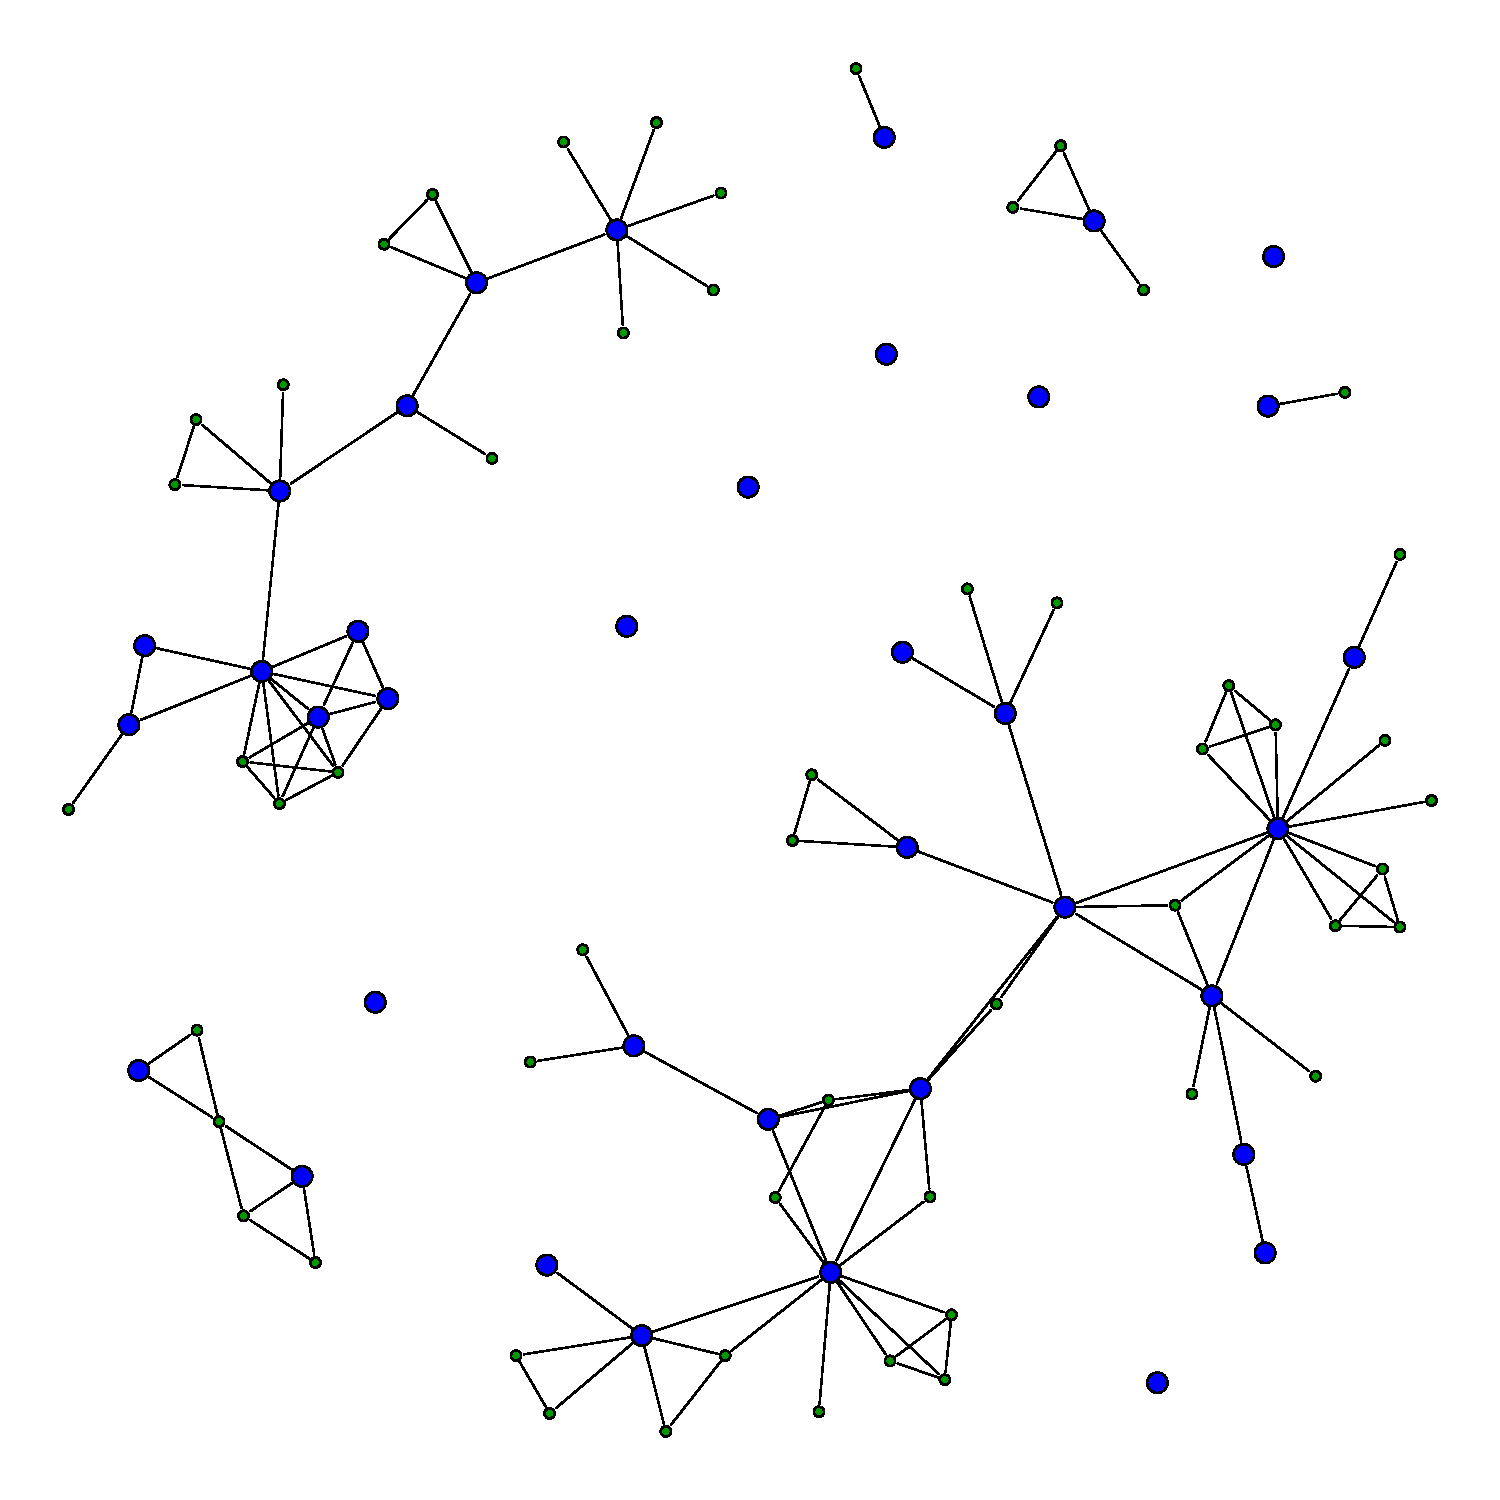
\includegraphics[width=.8\textwidth]{exemplo-grafo}
    \caption{Uma figura simples.\label{fig:subfigures:a}}
  \end{subfigure}
  % ATENÇÃO: Se você deixar uma linha em branco entre as subfiguras,
  % LaTeX vai considerar que cada uma delas pertence a um "parágrafo"
  % diferente e, portanto, vai colocá-las em linhas separadas ao invés
  % de lado a lado.
  \begin{subfigure}{0.4\textwidth}
    \centering
    \begin{turn}{90} % package rotating
      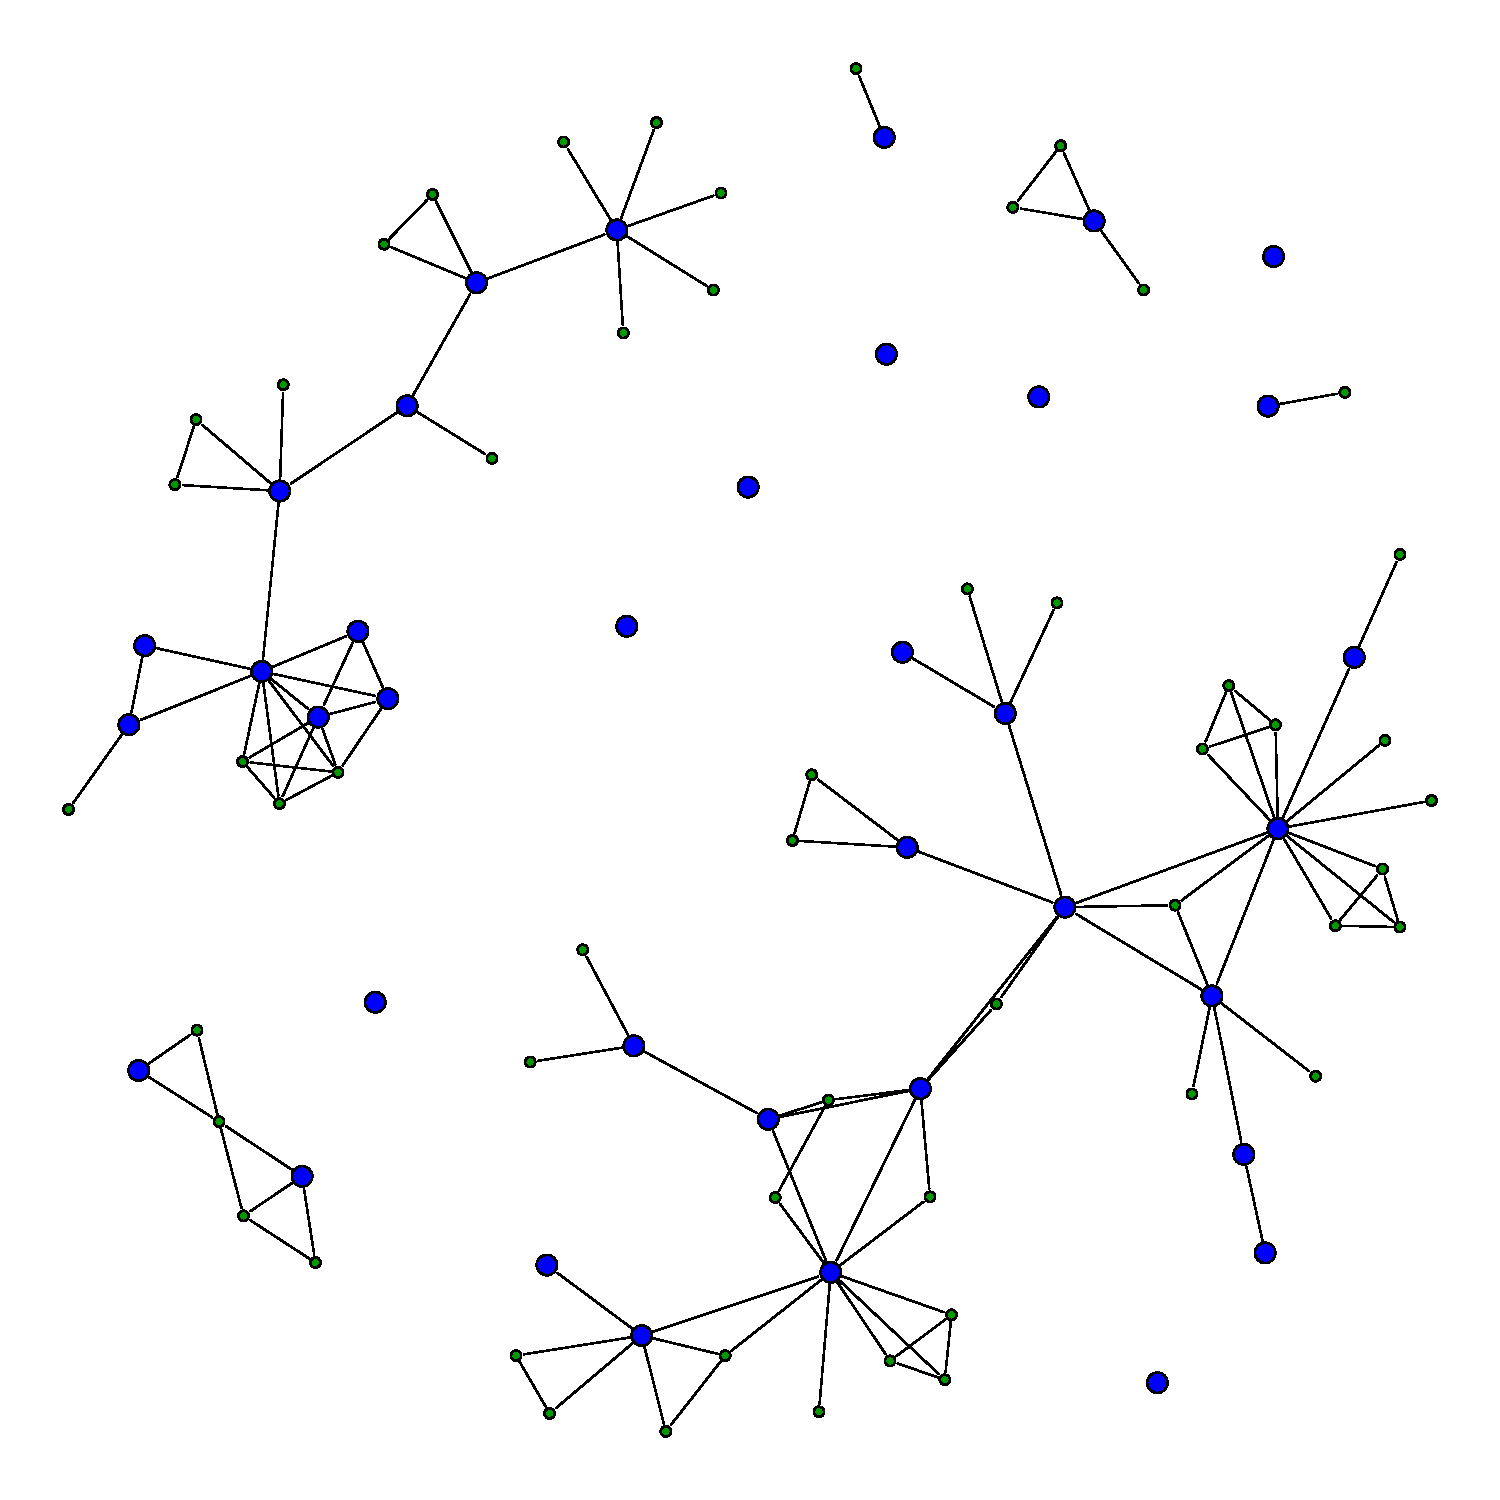
\includegraphics[width=.8\textwidth]{exemplo-grafo}
    \end{turn}
    \caption{O mesmo exemplo, girado.\label{fig:subfigures:b}}
  \end{subfigure}

  \caption{Exemplo de subfiguras.\label{fig:subfigures}}
\end{figure}

\emph{Floats} em geral incluem uma legenda e um \emph{label}.
Prefira sempre colocar o comando \textsf{\textbackslash{}label} de uma
figura ou tabela dentro do comando \textsf{\textbackslash{}caption};
não fazê-lo muitas vezes funciona, mas às vezes causa problemas.

Você pode carregar arquivos de imagem de um subdiretório usando
\texttt{dir/img.pdf}, mas é mais fácil modificar o comando
\textsf{\textbackslash{}graphicspath} próximo ao início de cada
arquivo~\texttt{.tex} de exemplo.

Para centralizar uma imagem mais larga que o texto da página, use
a \emph{package} \textsf{adjustbox} (incluída neste modelo):

\begin{verbatim}
  \begin{figure}
  \adjustbox{center}{\includegraphics[width=1.2\textwidth]{img.pdf}}
  \caption{...}
  \end{figure}
\end{verbatim}

Uma ``figura'', na verdade, pode ser qualquer tipo de conteúdo ilustrativo
(um exemplo interessante é o cronograma mostrado na Figura~\ref{fig:gantt})
mas, com a \textit{package} \textsf{float}, também é possível definir ambientes
específicos para cada tipo de conteúdo adicional (cada um com numeração
independente), como é o caso do Programa~\ref{prog:java}\index{Floats}. Há
mais informações e dicas sobre recursos específicos para inclusão de
código-fonte e pseudocódigo no Anexo\linebreak\ref{ap:pseudocode}\footnote{
Observe que o nome do Anexo (``\ref{ap:pseudocode}'') foi impresso em
uma linha separada, o que não é muito bom visualmente. Para evitar que isso
aconteça (não só no final do parágrafo, mas em qualquer quebra de linha),
utilize um espaço não-separável para fazer referências a figuras, tabelas,
seções etc. ou antes de símbolos: ``\textsf{\dots no
Anexo\textasciitilde\textbackslash{}ref\{ap:pseudocode\}}'',
``\textsf{O discriminante é denotado
por\textasciitilde{}\$\textbackslash{}Delta\$}''.}.

%%%%%%% Cronograma %%%%%%%

\begin{figure}
  \centering

  % Package pgfgantt; veja o arquivo imegoodies.sty, em que vários
  % aspectos da aparência deste diagrama foram definidos.
  \begin{ganttchart}[
                     time slot format=isodate-yearmonth,
                     time slot unit=month,
                    ]{2017-11}{2018-5}

    \gantttitlecalendar{year,month=shortname} \ganttnewline

    \ganttgroup[progress=45]{Experimento}{2017-11}{2018-2} \ganttnewline
    \ganttbar[progress=100]{
      Preparação\ganttalignnewline
      (compra de insumos)
      }{2017-11}{2017-12} \ganttnewline
    \ganttbar[progress=30]{Execução}{2017-12}{2018-1} \ganttnewline
    \ganttbar[progress=0]{Análise}{2017-12}{2018-2} \ganttnewline

    \ganttgroup[progress=0]{Artigo}{2018-1}{2018-4} \ganttnewline
    \ganttbar[progress=0]{Escrita}{2018-1}{2018-3} \ganttnewline
    \ganttbar[progress=0]{Revisão}{2018-3}{2018-4} \ganttnewline

    \ganttmilestone{Submissão}{2018-4}
  \end{ganttchart}

  \caption{Exemplo de cronograma.\label{fig:gantt}}
\end{figure}

%%%%%%%% Código fonte %%%%%%%%

% Foi utilizado o pacote listings para formatar o código fonte.
% Veja os parâmetros de configuração no arquivo source-code.tex.
\begin{program}
  \index{Java}
  \centering

\begin{lstlisting}[language=Java, style=wider]
  for (i = 0; i < 20; i++)
  {
      // Comentário
      System.out.println("Mensagem...");
  }
\end{lstlisting}

  \caption{Exemplo de laço em Java.\label{prog:java}}
\end{program}

%%%%%

\LaTeX{} também é capaz de gerar ilustrações e diagramas diretamente, mas
usar esses recursos em geral não é trivial. Em particular, a package
\textsf{tikz} oferece bons mecanismos para a criação de figuras (incluindo
funções pré-prontas para formas geométricas, grafos, matrizes etc.) e é
fácil usá-la para traçar linhas ou curvas simples.

Gráficos de dados ou funções matemáticas de excelente qualidade podem ser
gerados com a \textit{package} \pkg{pgfplots} (há um exemplo comentado neste
arquivo; experimente des-comentar para ver o resultado). Também é possível
importar gráficos gerados por \cmd{matplotlib}, \cmd{gnuplot} e \cmd{R}
como qualquer outra imagem, mas nesse caso a fonte usada nesses gráficos
provavelmente será diferente do corpo do texto. Felizmente, isso pode ser
solucionado: \cmd{Gnuplot} (com o \emph{driver} \cmd{lua tikz}\footnote{
\url{gnuplot.info/docs_5.5/loc20850.html}}),
\cmd{matplotlib} (com o \emph{backend} \textsc{pgf}\footnote{\url
{matplotlib.org/users/pgf.html}})
e \cmd{R} (com \cmd{tikzDevice}\footnote{\url
{cran.r-project.org/package=tikzDevice}}) são capazes de exportar gráficos de
dados na forma de comandos para \pkg{tikz}\footnote{Você pode se interessar
também pela \textit{package} \texttt{gnuplottex}.}: o resultado pode ser
visto na Figura~\ref{fig:graficos}.

\begin{figure}
  \centering
  \begin{subfigure}[b]{.45\textwidth}
    \input{figuras/gnuplot.tkz} % Exemplo com gnuplot
    %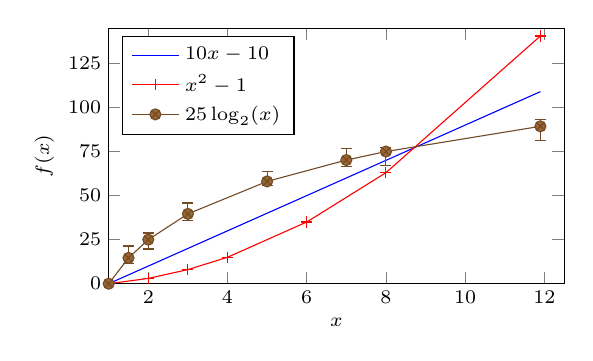
\begin{tikzpicture}
  \sffamily\scriptsize
  \begin{axis}[
    width=2.9in, height=1.9in,
    %title=Algum título,
    ylabel=$f(x)$,
    xlabel=$x$,
    xmin = 1,
    ymin = 0,
    xmax = 12.5,
    ymax = 145,
    ytick distance = 25,
    legend pos = north west,
    legend cell align = left,
  ]

  \addlegendentry{$10x-10$}
  \addplot+ [no marks] table
  {
     1.0   0
     2.0  10
     5.0  40
     7.0  60
    10.0  90
    11.9 109
  };

  \addlegendentry{$x^2-1$}
  \addplot+ [mark = +] table
  {
     1.0   0.0
     2.0   3.0
     3.0   8.0
     4.0  15.0
     6.0  35.0
     8.0  63.0
    11.9 140.6
  };
  \addlegendentry{$25\log_{2}(x)$}
  \addplot+ [error bars/y dir=both, error bars/y explicit,]
      table [y error minus index=2, y error plus index=3,]
  {
     1.0  0.00 0.0 0.0
     1.5 14.62 3.1 6.8
     2.0 25.00 5.3 3.8
     3.0 39.62 3.7 6.2
     5.0 58.05 2.2 5.5
     7.0 70.18 3.9 6.6
     8.0 75.00 7.9 2.3
    11.9 89.32 7.9 3.8
  };
  \end{axis}
\end{tikzpicture}
 % Exemplo com pgfplots
    \caption{\texttt{gnuplot}.\label{fig:gnuplot}}
  \end{subfigure}
  \begin{subfigure}[b]{.5\textwidth}
    %% Creator: Matplotlib, PGF backend
%%
%% To include the figure in your LaTeX document, write
%%   \input{<filename>.pgf}
%%
%% Make sure the required packages are loaded in your preamble
%%   \usepackage{pgf}
%%
%% and, on pdftex
%%   \usepackage[utf8]{inputenc}\DeclareUnicodeCharacter{2212}{-}
%%
%% or, on luatex and xetex
%%   \usepackage{unicode-math}
%%
%% Figures using additional raster images can only be included by \input if
%% they are in the same directory as the main LaTeX file. For loading figures
%% from other directories you can use the `import` package
%%   \usepackage{import}
%%
%% and then include the figures with
%%   \import{<path to file>}{<filename>.pgf}
%%
%% Matplotlib used the following preamble
%%   \usepackage{fontspec}
%%   \setmainfont{DejaVuSerif.ttf}[Path=/usr/share/matplotlib/mpl-data/fonts/ttf/]
%%   \setsansfont{DejaVuSans.ttf}[Path=/usr/share/matplotlib/mpl-data/fonts/ttf/]
%%   \setmonofont{DejaVuSansMono.ttf}[Path=/usr/share/matplotlib/mpl-data/fonts/ttf/]
%%
\begingroup%
\makeatletter%
\begin{pgfpicture}%
\pgfpathrectangle{\pgfpointorigin}{\pgfqpoint{2.900000in}{1.800000in}}%
\pgfusepath{use as bounding box, clip}%
\begin{pgfscope}%
\pgfsetbuttcap%
\pgfsetmiterjoin%
\definecolor{currentfill}{rgb}{1.000000,1.000000,1.000000}%
\pgfsetfillcolor{currentfill}%
\pgfsetlinewidth{0.000000pt}%
\definecolor{currentstroke}{rgb}{1.000000,1.000000,1.000000}%
\pgfsetstrokecolor{currentstroke}%
\pgfsetdash{}{0pt}%
\pgfpathmoveto{\pgfqpoint{0.000000in}{0.000000in}}%
\pgfpathlineto{\pgfqpoint{2.900000in}{0.000000in}}%
\pgfpathlineto{\pgfqpoint{2.900000in}{1.800000in}}%
\pgfpathlineto{\pgfqpoint{0.000000in}{1.800000in}}%
\pgfpathclose%
\pgfusepath{fill}%
\end{pgfscope}%
\begin{pgfscope}%
\pgfsetbuttcap%
\pgfsetmiterjoin%
\definecolor{currentfill}{rgb}{1.000000,1.000000,1.000000}%
\pgfsetfillcolor{currentfill}%
\pgfsetlinewidth{0.000000pt}%
\definecolor{currentstroke}{rgb}{0.000000,0.000000,0.000000}%
\pgfsetstrokecolor{currentstroke}%
\pgfsetstrokeopacity{0.000000}%
\pgfsetdash{}{0pt}%
\pgfpathmoveto{\pgfqpoint{0.616528in}{0.472778in}}%
\pgfpathlineto{\pgfqpoint{2.780000in}{0.472778in}}%
\pgfpathlineto{\pgfqpoint{2.780000in}{1.680000in}}%
\pgfpathlineto{\pgfqpoint{0.616528in}{1.680000in}}%
\pgfpathclose%
\pgfusepath{fill}%
\end{pgfscope}%
\begin{pgfscope}%
\pgfsetbuttcap%
\pgfsetroundjoin%
\definecolor{currentfill}{rgb}{0.000000,0.000000,0.000000}%
\pgfsetfillcolor{currentfill}%
\pgfsetlinewidth{0.803000pt}%
\definecolor{currentstroke}{rgb}{0.000000,0.000000,0.000000}%
\pgfsetstrokecolor{currentstroke}%
\pgfsetdash{}{0pt}%
\pgfsys@defobject{currentmarker}{\pgfqpoint{0.000000in}{-0.048611in}}{\pgfqpoint{0.000000in}{0.000000in}}{%
\pgfpathmoveto{\pgfqpoint{0.000000in}{0.000000in}}%
\pgfpathlineto{\pgfqpoint{0.000000in}{-0.048611in}}%
\pgfusepath{stroke,fill}%
}%
\begin{pgfscope}%
\pgfsys@transformshift{0.804656in}{0.472778in}%
\pgfsys@useobject{currentmarker}{}%
\end{pgfscope}%
\end{pgfscope}%
\begin{pgfscope}%
\definecolor{textcolor}{rgb}{0.000000,0.000000,0.000000}%
\pgfsetstrokecolor{textcolor}%
\pgfsetfillcolor{textcolor}%
\pgftext[x=0.804656in,y=0.375556in,,top]{\color{textcolor}\sffamily\fontsize{8.000000}{9.600000}\selectfont 2}%
\end{pgfscope}%
\begin{pgfscope}%
\pgfsetbuttcap%
\pgfsetroundjoin%
\definecolor{currentfill}{rgb}{0.000000,0.000000,0.000000}%
\pgfsetfillcolor{currentfill}%
\pgfsetlinewidth{0.803000pt}%
\definecolor{currentstroke}{rgb}{0.000000,0.000000,0.000000}%
\pgfsetstrokecolor{currentstroke}%
\pgfsetdash{}{0pt}%
\pgfsys@defobject{currentmarker}{\pgfqpoint{0.000000in}{-0.048611in}}{\pgfqpoint{0.000000in}{0.000000in}}{%
\pgfpathmoveto{\pgfqpoint{0.000000in}{0.000000in}}%
\pgfpathlineto{\pgfqpoint{0.000000in}{-0.048611in}}%
\pgfusepath{stroke,fill}%
}%
\begin{pgfscope}%
\pgfsys@transformshift{1.180912in}{0.472778in}%
\pgfsys@useobject{currentmarker}{}%
\end{pgfscope}%
\end{pgfscope}%
\begin{pgfscope}%
\definecolor{textcolor}{rgb}{0.000000,0.000000,0.000000}%
\pgfsetstrokecolor{textcolor}%
\pgfsetfillcolor{textcolor}%
\pgftext[x=1.180912in,y=0.375556in,,top]{\color{textcolor}\sffamily\fontsize{8.000000}{9.600000}\selectfont 4}%
\end{pgfscope}%
\begin{pgfscope}%
\pgfsetbuttcap%
\pgfsetroundjoin%
\definecolor{currentfill}{rgb}{0.000000,0.000000,0.000000}%
\pgfsetfillcolor{currentfill}%
\pgfsetlinewidth{0.803000pt}%
\definecolor{currentstroke}{rgb}{0.000000,0.000000,0.000000}%
\pgfsetstrokecolor{currentstroke}%
\pgfsetdash{}{0pt}%
\pgfsys@defobject{currentmarker}{\pgfqpoint{0.000000in}{-0.048611in}}{\pgfqpoint{0.000000in}{0.000000in}}{%
\pgfpathmoveto{\pgfqpoint{0.000000in}{0.000000in}}%
\pgfpathlineto{\pgfqpoint{0.000000in}{-0.048611in}}%
\pgfusepath{stroke,fill}%
}%
\begin{pgfscope}%
\pgfsys@transformshift{1.557168in}{0.472778in}%
\pgfsys@useobject{currentmarker}{}%
\end{pgfscope}%
\end{pgfscope}%
\begin{pgfscope}%
\definecolor{textcolor}{rgb}{0.000000,0.000000,0.000000}%
\pgfsetstrokecolor{textcolor}%
\pgfsetfillcolor{textcolor}%
\pgftext[x=1.557168in,y=0.375556in,,top]{\color{textcolor}\sffamily\fontsize{8.000000}{9.600000}\selectfont 6}%
\end{pgfscope}%
\begin{pgfscope}%
\pgfsetbuttcap%
\pgfsetroundjoin%
\definecolor{currentfill}{rgb}{0.000000,0.000000,0.000000}%
\pgfsetfillcolor{currentfill}%
\pgfsetlinewidth{0.803000pt}%
\definecolor{currentstroke}{rgb}{0.000000,0.000000,0.000000}%
\pgfsetstrokecolor{currentstroke}%
\pgfsetdash{}{0pt}%
\pgfsys@defobject{currentmarker}{\pgfqpoint{0.000000in}{-0.048611in}}{\pgfqpoint{0.000000in}{0.000000in}}{%
\pgfpathmoveto{\pgfqpoint{0.000000in}{0.000000in}}%
\pgfpathlineto{\pgfqpoint{0.000000in}{-0.048611in}}%
\pgfusepath{stroke,fill}%
}%
\begin{pgfscope}%
\pgfsys@transformshift{1.933424in}{0.472778in}%
\pgfsys@useobject{currentmarker}{}%
\end{pgfscope}%
\end{pgfscope}%
\begin{pgfscope}%
\definecolor{textcolor}{rgb}{0.000000,0.000000,0.000000}%
\pgfsetstrokecolor{textcolor}%
\pgfsetfillcolor{textcolor}%
\pgftext[x=1.933424in,y=0.375556in,,top]{\color{textcolor}\sffamily\fontsize{8.000000}{9.600000}\selectfont 8}%
\end{pgfscope}%
\begin{pgfscope}%
\pgfsetbuttcap%
\pgfsetroundjoin%
\definecolor{currentfill}{rgb}{0.000000,0.000000,0.000000}%
\pgfsetfillcolor{currentfill}%
\pgfsetlinewidth{0.803000pt}%
\definecolor{currentstroke}{rgb}{0.000000,0.000000,0.000000}%
\pgfsetstrokecolor{currentstroke}%
\pgfsetdash{}{0pt}%
\pgfsys@defobject{currentmarker}{\pgfqpoint{0.000000in}{-0.048611in}}{\pgfqpoint{0.000000in}{0.000000in}}{%
\pgfpathmoveto{\pgfqpoint{0.000000in}{0.000000in}}%
\pgfpathlineto{\pgfqpoint{0.000000in}{-0.048611in}}%
\pgfusepath{stroke,fill}%
}%
\begin{pgfscope}%
\pgfsys@transformshift{2.309680in}{0.472778in}%
\pgfsys@useobject{currentmarker}{}%
\end{pgfscope}%
\end{pgfscope}%
\begin{pgfscope}%
\definecolor{textcolor}{rgb}{0.000000,0.000000,0.000000}%
\pgfsetstrokecolor{textcolor}%
\pgfsetfillcolor{textcolor}%
\pgftext[x=2.309680in,y=0.375556in,,top]{\color{textcolor}\sffamily\fontsize{8.000000}{9.600000}\selectfont 10}%
\end{pgfscope}%
\begin{pgfscope}%
\pgfsetbuttcap%
\pgfsetroundjoin%
\definecolor{currentfill}{rgb}{0.000000,0.000000,0.000000}%
\pgfsetfillcolor{currentfill}%
\pgfsetlinewidth{0.803000pt}%
\definecolor{currentstroke}{rgb}{0.000000,0.000000,0.000000}%
\pgfsetstrokecolor{currentstroke}%
\pgfsetdash{}{0pt}%
\pgfsys@defobject{currentmarker}{\pgfqpoint{0.000000in}{-0.048611in}}{\pgfqpoint{0.000000in}{0.000000in}}{%
\pgfpathmoveto{\pgfqpoint{0.000000in}{0.000000in}}%
\pgfpathlineto{\pgfqpoint{0.000000in}{-0.048611in}}%
\pgfusepath{stroke,fill}%
}%
\begin{pgfscope}%
\pgfsys@transformshift{2.685936in}{0.472778in}%
\pgfsys@useobject{currentmarker}{}%
\end{pgfscope}%
\end{pgfscope}%
\begin{pgfscope}%
\definecolor{textcolor}{rgb}{0.000000,0.000000,0.000000}%
\pgfsetstrokecolor{textcolor}%
\pgfsetfillcolor{textcolor}%
\pgftext[x=2.685936in,y=0.375556in,,top]{\color{textcolor}\sffamily\fontsize{8.000000}{9.600000}\selectfont 12}%
\end{pgfscope}%
\begin{pgfscope}%
\definecolor{textcolor}{rgb}{0.000000,0.000000,0.000000}%
\pgfsetstrokecolor{textcolor}%
\pgfsetfillcolor{textcolor}%
\pgftext[x=1.698264in,y=0.212470in,,top]{\color{textcolor}\sffamily\fontsize{8.000000}{9.600000}\selectfont \(\displaystyle x\)}%
\end{pgfscope}%
\begin{pgfscope}%
\pgfsetbuttcap%
\pgfsetroundjoin%
\definecolor{currentfill}{rgb}{0.000000,0.000000,0.000000}%
\pgfsetfillcolor{currentfill}%
\pgfsetlinewidth{0.803000pt}%
\definecolor{currentstroke}{rgb}{0.000000,0.000000,0.000000}%
\pgfsetstrokecolor{currentstroke}%
\pgfsetdash{}{0pt}%
\pgfsys@defobject{currentmarker}{\pgfqpoint{-0.048611in}{0.000000in}}{\pgfqpoint{-0.000000in}{0.000000in}}{%
\pgfpathmoveto{\pgfqpoint{-0.000000in}{0.000000in}}%
\pgfpathlineto{\pgfqpoint{-0.048611in}{0.000000in}}%
\pgfusepath{stroke,fill}%
}%
\begin{pgfscope}%
\pgfsys@transformshift{0.616528in}{0.472778in}%
\pgfsys@useobject{currentmarker}{}%
\end{pgfscope}%
\end{pgfscope}%
\begin{pgfscope}%
\definecolor{textcolor}{rgb}{0.000000,0.000000,0.000000}%
\pgfsetstrokecolor{textcolor}%
\pgfsetfillcolor{textcolor}%
\pgftext[x=0.448613in, y=0.430569in, left, base]{\color{textcolor}\sffamily\fontsize{8.000000}{9.600000}\selectfont 0}%
\end{pgfscope}%
\begin{pgfscope}%
\pgfsetbuttcap%
\pgfsetroundjoin%
\definecolor{currentfill}{rgb}{0.000000,0.000000,0.000000}%
\pgfsetfillcolor{currentfill}%
\pgfsetlinewidth{0.803000pt}%
\definecolor{currentstroke}{rgb}{0.000000,0.000000,0.000000}%
\pgfsetstrokecolor{currentstroke}%
\pgfsetdash{}{0pt}%
\pgfsys@defobject{currentmarker}{\pgfqpoint{-0.048611in}{0.000000in}}{\pgfqpoint{-0.000000in}{0.000000in}}{%
\pgfpathmoveto{\pgfqpoint{-0.000000in}{0.000000in}}%
\pgfpathlineto{\pgfqpoint{-0.048611in}{0.000000in}}%
\pgfusepath{stroke,fill}%
}%
\begin{pgfscope}%
\pgfsys@transformshift{0.616528in}{0.680920in}%
\pgfsys@useobject{currentmarker}{}%
\end{pgfscope}%
\end{pgfscope}%
\begin{pgfscope}%
\definecolor{textcolor}{rgb}{0.000000,0.000000,0.000000}%
\pgfsetstrokecolor{textcolor}%
\pgfsetfillcolor{textcolor}%
\pgftext[x=0.377921in, y=0.638710in, left, base]{\color{textcolor}\sffamily\fontsize{8.000000}{9.600000}\selectfont 25}%
\end{pgfscope}%
\begin{pgfscope}%
\pgfsetbuttcap%
\pgfsetroundjoin%
\definecolor{currentfill}{rgb}{0.000000,0.000000,0.000000}%
\pgfsetfillcolor{currentfill}%
\pgfsetlinewidth{0.803000pt}%
\definecolor{currentstroke}{rgb}{0.000000,0.000000,0.000000}%
\pgfsetstrokecolor{currentstroke}%
\pgfsetdash{}{0pt}%
\pgfsys@defobject{currentmarker}{\pgfqpoint{-0.048611in}{0.000000in}}{\pgfqpoint{-0.000000in}{0.000000in}}{%
\pgfpathmoveto{\pgfqpoint{-0.000000in}{0.000000in}}%
\pgfpathlineto{\pgfqpoint{-0.048611in}{0.000000in}}%
\pgfusepath{stroke,fill}%
}%
\begin{pgfscope}%
\pgfsys@transformshift{0.616528in}{0.889061in}%
\pgfsys@useobject{currentmarker}{}%
\end{pgfscope}%
\end{pgfscope}%
\begin{pgfscope}%
\definecolor{textcolor}{rgb}{0.000000,0.000000,0.000000}%
\pgfsetstrokecolor{textcolor}%
\pgfsetfillcolor{textcolor}%
\pgftext[x=0.377921in, y=0.846852in, left, base]{\color{textcolor}\sffamily\fontsize{8.000000}{9.600000}\selectfont 50}%
\end{pgfscope}%
\begin{pgfscope}%
\pgfsetbuttcap%
\pgfsetroundjoin%
\definecolor{currentfill}{rgb}{0.000000,0.000000,0.000000}%
\pgfsetfillcolor{currentfill}%
\pgfsetlinewidth{0.803000pt}%
\definecolor{currentstroke}{rgb}{0.000000,0.000000,0.000000}%
\pgfsetstrokecolor{currentstroke}%
\pgfsetdash{}{0pt}%
\pgfsys@defobject{currentmarker}{\pgfqpoint{-0.048611in}{0.000000in}}{\pgfqpoint{-0.000000in}{0.000000in}}{%
\pgfpathmoveto{\pgfqpoint{-0.000000in}{0.000000in}}%
\pgfpathlineto{\pgfqpoint{-0.048611in}{0.000000in}}%
\pgfusepath{stroke,fill}%
}%
\begin{pgfscope}%
\pgfsys@transformshift{0.616528in}{1.097203in}%
\pgfsys@useobject{currentmarker}{}%
\end{pgfscope}%
\end{pgfscope}%
\begin{pgfscope}%
\definecolor{textcolor}{rgb}{0.000000,0.000000,0.000000}%
\pgfsetstrokecolor{textcolor}%
\pgfsetfillcolor{textcolor}%
\pgftext[x=0.377921in, y=1.054994in, left, base]{\color{textcolor}\sffamily\fontsize{8.000000}{9.600000}\selectfont 75}%
\end{pgfscope}%
\begin{pgfscope}%
\pgfsetbuttcap%
\pgfsetroundjoin%
\definecolor{currentfill}{rgb}{0.000000,0.000000,0.000000}%
\pgfsetfillcolor{currentfill}%
\pgfsetlinewidth{0.803000pt}%
\definecolor{currentstroke}{rgb}{0.000000,0.000000,0.000000}%
\pgfsetstrokecolor{currentstroke}%
\pgfsetdash{}{0pt}%
\pgfsys@defobject{currentmarker}{\pgfqpoint{-0.048611in}{0.000000in}}{\pgfqpoint{-0.000000in}{0.000000in}}{%
\pgfpathmoveto{\pgfqpoint{-0.000000in}{0.000000in}}%
\pgfpathlineto{\pgfqpoint{-0.048611in}{0.000000in}}%
\pgfusepath{stroke,fill}%
}%
\begin{pgfscope}%
\pgfsys@transformshift{0.616528in}{1.305345in}%
\pgfsys@useobject{currentmarker}{}%
\end{pgfscope}%
\end{pgfscope}%
\begin{pgfscope}%
\definecolor{textcolor}{rgb}{0.000000,0.000000,0.000000}%
\pgfsetstrokecolor{textcolor}%
\pgfsetfillcolor{textcolor}%
\pgftext[x=0.307229in, y=1.263136in, left, base]{\color{textcolor}\sffamily\fontsize{8.000000}{9.600000}\selectfont 100}%
\end{pgfscope}%
\begin{pgfscope}%
\pgfsetbuttcap%
\pgfsetroundjoin%
\definecolor{currentfill}{rgb}{0.000000,0.000000,0.000000}%
\pgfsetfillcolor{currentfill}%
\pgfsetlinewidth{0.803000pt}%
\definecolor{currentstroke}{rgb}{0.000000,0.000000,0.000000}%
\pgfsetstrokecolor{currentstroke}%
\pgfsetdash{}{0pt}%
\pgfsys@defobject{currentmarker}{\pgfqpoint{-0.048611in}{0.000000in}}{\pgfqpoint{-0.000000in}{0.000000in}}{%
\pgfpathmoveto{\pgfqpoint{-0.000000in}{0.000000in}}%
\pgfpathlineto{\pgfqpoint{-0.048611in}{0.000000in}}%
\pgfusepath{stroke,fill}%
}%
\begin{pgfscope}%
\pgfsys@transformshift{0.616528in}{1.513487in}%
\pgfsys@useobject{currentmarker}{}%
\end{pgfscope}%
\end{pgfscope}%
\begin{pgfscope}%
\definecolor{textcolor}{rgb}{0.000000,0.000000,0.000000}%
\pgfsetstrokecolor{textcolor}%
\pgfsetfillcolor{textcolor}%
\pgftext[x=0.307229in, y=1.471277in, left, base]{\color{textcolor}\sffamily\fontsize{8.000000}{9.600000}\selectfont 125}%
\end{pgfscope}%
\begin{pgfscope}%
\definecolor{textcolor}{rgb}{0.000000,0.000000,0.000000}%
\pgfsetstrokecolor{textcolor}%
\pgfsetfillcolor{textcolor}%
\pgftext[x=0.251673in,y=1.076389in,,bottom,rotate=90.000000]{\color{textcolor}\sffamily\fontsize{8.000000}{9.600000}\selectfont \(\displaystyle f(x)\)}%
\end{pgfscope}%
\begin{pgfscope}%
\pgfpathrectangle{\pgfqpoint{0.616528in}{0.472778in}}{\pgfqpoint{2.163472in}{1.207222in}}%
\pgfusepath{clip}%
\pgfsetbuttcap%
\pgfsetroundjoin%
\pgfsetlinewidth{0.501875pt}%
\definecolor{currentstroke}{rgb}{0.172549,0.627451,0.172549}%
\pgfsetstrokecolor{currentstroke}%
\pgfsetdash{}{0pt}%
\pgfpathmoveto{\pgfqpoint{0.616528in}{0.472778in}}%
\pgfpathlineto{\pgfqpoint{0.616528in}{0.472778in}}%
\pgfusepath{stroke}%
\end{pgfscope}%
\begin{pgfscope}%
\pgfpathrectangle{\pgfqpoint{0.616528in}{0.472778in}}{\pgfqpoint{2.163472in}{1.207222in}}%
\pgfusepath{clip}%
\pgfsetbuttcap%
\pgfsetroundjoin%
\pgfsetlinewidth{0.501875pt}%
\definecolor{currentstroke}{rgb}{0.172549,0.627451,0.172549}%
\pgfsetstrokecolor{currentstroke}%
\pgfsetdash{}{0pt}%
\pgfpathmoveto{\pgfqpoint{0.710592in}{0.568690in}}%
\pgfpathlineto{\pgfqpoint{0.710592in}{0.651114in}}%
\pgfusepath{stroke}%
\end{pgfscope}%
\begin{pgfscope}%
\pgfpathrectangle{\pgfqpoint{0.616528in}{0.472778in}}{\pgfqpoint{2.163472in}{1.207222in}}%
\pgfusepath{clip}%
\pgfsetbuttcap%
\pgfsetroundjoin%
\pgfsetlinewidth{0.501875pt}%
\definecolor{currentstroke}{rgb}{0.172549,0.627451,0.172549}%
\pgfsetstrokecolor{currentstroke}%
\pgfsetdash{}{0pt}%
\pgfpathmoveto{\pgfqpoint{0.804656in}{0.636793in}}%
\pgfpathlineto{\pgfqpoint{0.804656in}{0.712557in}}%
\pgfusepath{stroke}%
\end{pgfscope}%
\begin{pgfscope}%
\pgfpathrectangle{\pgfqpoint{0.616528in}{0.472778in}}{\pgfqpoint{2.163472in}{1.207222in}}%
\pgfusepath{clip}%
\pgfsetbuttcap%
\pgfsetroundjoin%
\pgfsetlinewidth{0.501875pt}%
\definecolor{currentstroke}{rgb}{0.172549,0.627451,0.172549}%
\pgfsetstrokecolor{currentstroke}%
\pgfsetdash{}{0pt}%
\pgfpathmoveto{\pgfqpoint{0.992784in}{0.771836in}}%
\pgfpathlineto{\pgfqpoint{0.992784in}{0.854260in}}%
\pgfusepath{stroke}%
\end{pgfscope}%
\begin{pgfscope}%
\pgfpathrectangle{\pgfqpoint{0.616528in}{0.472778in}}{\pgfqpoint{2.163472in}{1.207222in}}%
\pgfusepath{clip}%
\pgfsetbuttcap%
\pgfsetroundjoin%
\pgfsetlinewidth{0.501875pt}%
\definecolor{currentstroke}{rgb}{0.172549,0.627451,0.172549}%
\pgfsetstrokecolor{currentstroke}%
\pgfsetdash{}{0pt}%
\pgfpathmoveto{\pgfqpoint{1.369040in}{0.937766in}}%
\pgfpathlineto{\pgfqpoint{1.369040in}{1.001874in}}%
\pgfusepath{stroke}%
\end{pgfscope}%
\begin{pgfscope}%
\pgfpathrectangle{\pgfqpoint{0.616528in}{0.472778in}}{\pgfqpoint{2.163472in}{1.207222in}}%
\pgfusepath{clip}%
\pgfsetbuttcap%
\pgfsetroundjoin%
\pgfsetlinewidth{0.501875pt}%
\definecolor{currentstroke}{rgb}{0.172549,0.627451,0.172549}%
\pgfsetstrokecolor{currentstroke}%
\pgfsetdash{}{0pt}%
\pgfpathmoveto{\pgfqpoint{1.745296in}{1.024603in}}%
\pgfpathlineto{\pgfqpoint{1.745296in}{1.112023in}}%
\pgfusepath{stroke}%
\end{pgfscope}%
\begin{pgfscope}%
\pgfpathrectangle{\pgfqpoint{0.616528in}{0.472778in}}{\pgfqpoint{2.163472in}{1.207222in}}%
\pgfusepath{clip}%
\pgfsetbuttcap%
\pgfsetroundjoin%
\pgfsetlinewidth{0.501875pt}%
\definecolor{currentstroke}{rgb}{0.172549,0.627451,0.172549}%
\pgfsetstrokecolor{currentstroke}%
\pgfsetdash{}{0pt}%
\pgfpathmoveto{\pgfqpoint{1.933424in}{1.031430in}}%
\pgfpathlineto{\pgfqpoint{1.933424in}{1.116352in}}%
\pgfusepath{stroke}%
\end{pgfscope}%
\begin{pgfscope}%
\pgfpathrectangle{\pgfqpoint{0.616528in}{0.472778in}}{\pgfqpoint{2.163472in}{1.207222in}}%
\pgfusepath{clip}%
\pgfsetbuttcap%
\pgfsetroundjoin%
\pgfsetlinewidth{0.501875pt}%
\definecolor{currentstroke}{rgb}{0.172549,0.627451,0.172549}%
\pgfsetstrokecolor{currentstroke}%
\pgfsetdash{}{0pt}%
\pgfpathmoveto{\pgfqpoint{2.667123in}{1.150654in}}%
\pgfpathlineto{\pgfqpoint{2.667123in}{1.248064in}}%
\pgfusepath{stroke}%
\end{pgfscope}%
\begin{pgfscope}%
\pgfpathrectangle{\pgfqpoint{0.616528in}{0.472778in}}{\pgfqpoint{2.163472in}{1.207222in}}%
\pgfusepath{clip}%
\pgfsetrectcap%
\pgfsetroundjoin%
\pgfsetlinewidth{1.003750pt}%
\definecolor{currentstroke}{rgb}{0.121569,0.466667,0.705882}%
\pgfsetstrokecolor{currentstroke}%
\pgfsetdash{}{0pt}%
\pgfpathmoveto{\pgfqpoint{0.616528in}{0.472778in}}%
\pgfpathlineto{\pgfqpoint{0.635341in}{0.481103in}}%
\pgfpathlineto{\pgfqpoint{0.654153in}{0.489429in}}%
\pgfpathlineto{\pgfqpoint{0.672966in}{0.497755in}}%
\pgfpathlineto{\pgfqpoint{0.691779in}{0.506080in}}%
\pgfpathlineto{\pgfqpoint{0.710592in}{0.514406in}}%
\pgfpathlineto{\pgfqpoint{0.729405in}{0.522732in}}%
\pgfpathlineto{\pgfqpoint{0.748217in}{0.531057in}}%
\pgfpathlineto{\pgfqpoint{0.767030in}{0.539383in}}%
\pgfpathlineto{\pgfqpoint{0.785843in}{0.547709in}}%
\pgfpathlineto{\pgfqpoint{0.804656in}{0.556034in}}%
\pgfpathlineto{\pgfqpoint{0.823469in}{0.564360in}}%
\pgfpathlineto{\pgfqpoint{0.842281in}{0.572686in}}%
\pgfpathlineto{\pgfqpoint{0.861094in}{0.581011in}}%
\pgfpathlineto{\pgfqpoint{0.879907in}{0.589337in}}%
\pgfpathlineto{\pgfqpoint{0.898720in}{0.597663in}}%
\pgfpathlineto{\pgfqpoint{0.917533in}{0.605989in}}%
\pgfpathlineto{\pgfqpoint{0.936345in}{0.614314in}}%
\pgfpathlineto{\pgfqpoint{0.955158in}{0.622640in}}%
\pgfpathlineto{\pgfqpoint{0.973971in}{0.630966in}}%
\pgfpathlineto{\pgfqpoint{0.992784in}{0.639291in}}%
\pgfpathlineto{\pgfqpoint{1.011597in}{0.647617in}}%
\pgfpathlineto{\pgfqpoint{1.030409in}{0.655943in}}%
\pgfpathlineto{\pgfqpoint{1.049222in}{0.664268in}}%
\pgfpathlineto{\pgfqpoint{1.068035in}{0.672594in}}%
\pgfpathlineto{\pgfqpoint{1.086848in}{0.680920in}}%
\pgfpathlineto{\pgfqpoint{1.105661in}{0.689245in}}%
\pgfpathlineto{\pgfqpoint{1.124473in}{0.697571in}}%
\pgfpathlineto{\pgfqpoint{1.143286in}{0.705897in}}%
\pgfpathlineto{\pgfqpoint{1.162099in}{0.714222in}}%
\pgfpathlineto{\pgfqpoint{1.180912in}{0.722548in}}%
\pgfpathlineto{\pgfqpoint{1.199725in}{0.730874in}}%
\pgfpathlineto{\pgfqpoint{1.218537in}{0.739199in}}%
\pgfpathlineto{\pgfqpoint{1.237350in}{0.747525in}}%
\pgfpathlineto{\pgfqpoint{1.256163in}{0.755851in}}%
\pgfpathlineto{\pgfqpoint{1.274976in}{0.764176in}}%
\pgfpathlineto{\pgfqpoint{1.293789in}{0.772502in}}%
\pgfpathlineto{\pgfqpoint{1.312601in}{0.780828in}}%
\pgfpathlineto{\pgfqpoint{1.331414in}{0.789153in}}%
\pgfpathlineto{\pgfqpoint{1.350227in}{0.797479in}}%
\pgfpathlineto{\pgfqpoint{1.369040in}{0.805805in}}%
\pgfpathlineto{\pgfqpoint{1.387853in}{0.814130in}}%
\pgfpathlineto{\pgfqpoint{1.406665in}{0.822456in}}%
\pgfpathlineto{\pgfqpoint{1.425478in}{0.830782in}}%
\pgfpathlineto{\pgfqpoint{1.444291in}{0.839107in}}%
\pgfpathlineto{\pgfqpoint{1.463104in}{0.847433in}}%
\pgfpathlineto{\pgfqpoint{1.481917in}{0.855759in}}%
\pgfpathlineto{\pgfqpoint{1.500729in}{0.864084in}}%
\pgfpathlineto{\pgfqpoint{1.519542in}{0.872410in}}%
\pgfpathlineto{\pgfqpoint{1.538355in}{0.880736in}}%
\pgfpathlineto{\pgfqpoint{1.557168in}{0.889061in}}%
\pgfpathlineto{\pgfqpoint{1.575981in}{0.897387in}}%
\pgfpathlineto{\pgfqpoint{1.594793in}{0.905713in}}%
\pgfpathlineto{\pgfqpoint{1.613606in}{0.914038in}}%
\pgfpathlineto{\pgfqpoint{1.632419in}{0.922364in}}%
\pgfpathlineto{\pgfqpoint{1.651232in}{0.930690in}}%
\pgfpathlineto{\pgfqpoint{1.670045in}{0.939015in}}%
\pgfpathlineto{\pgfqpoint{1.688857in}{0.947341in}}%
\pgfpathlineto{\pgfqpoint{1.707670in}{0.955667in}}%
\pgfpathlineto{\pgfqpoint{1.726483in}{0.963992in}}%
\pgfpathlineto{\pgfqpoint{1.745296in}{0.972318in}}%
\pgfpathlineto{\pgfqpoint{1.764109in}{0.980644in}}%
\pgfpathlineto{\pgfqpoint{1.782921in}{0.988969in}}%
\pgfpathlineto{\pgfqpoint{1.801734in}{0.997295in}}%
\pgfpathlineto{\pgfqpoint{1.820547in}{1.005621in}}%
\pgfpathlineto{\pgfqpoint{1.839360in}{1.013946in}}%
\pgfpathlineto{\pgfqpoint{1.858173in}{1.022272in}}%
\pgfpathlineto{\pgfqpoint{1.876986in}{1.030598in}}%
\pgfpathlineto{\pgfqpoint{1.895798in}{1.038923in}}%
\pgfpathlineto{\pgfqpoint{1.914611in}{1.047249in}}%
\pgfpathlineto{\pgfqpoint{1.933424in}{1.055575in}}%
\pgfpathlineto{\pgfqpoint{1.952237in}{1.063900in}}%
\pgfpathlineto{\pgfqpoint{1.971050in}{1.072226in}}%
\pgfpathlineto{\pgfqpoint{1.989862in}{1.080552in}}%
\pgfpathlineto{\pgfqpoint{2.008675in}{1.088877in}}%
\pgfpathlineto{\pgfqpoint{2.027488in}{1.097203in}}%
\pgfpathlineto{\pgfqpoint{2.046301in}{1.105529in}}%
\pgfpathlineto{\pgfqpoint{2.065114in}{1.113854in}}%
\pgfpathlineto{\pgfqpoint{2.083926in}{1.122180in}}%
\pgfpathlineto{\pgfqpoint{2.102739in}{1.130506in}}%
\pgfpathlineto{\pgfqpoint{2.121552in}{1.138831in}}%
\pgfpathlineto{\pgfqpoint{2.140365in}{1.147157in}}%
\pgfpathlineto{\pgfqpoint{2.159178in}{1.155483in}}%
\pgfpathlineto{\pgfqpoint{2.177990in}{1.163808in}}%
\pgfpathlineto{\pgfqpoint{2.196803in}{1.172134in}}%
\pgfpathlineto{\pgfqpoint{2.215616in}{1.180460in}}%
\pgfpathlineto{\pgfqpoint{2.234429in}{1.188785in}}%
\pgfpathlineto{\pgfqpoint{2.253242in}{1.197111in}}%
\pgfpathlineto{\pgfqpoint{2.272054in}{1.205437in}}%
\pgfpathlineto{\pgfqpoint{2.290867in}{1.213762in}}%
\pgfpathlineto{\pgfqpoint{2.309680in}{1.222088in}}%
\pgfpathlineto{\pgfqpoint{2.328493in}{1.230414in}}%
\pgfpathlineto{\pgfqpoint{2.347306in}{1.238739in}}%
\pgfpathlineto{\pgfqpoint{2.366118in}{1.247065in}}%
\pgfpathlineto{\pgfqpoint{2.384931in}{1.255391in}}%
\pgfpathlineto{\pgfqpoint{2.403744in}{1.263716in}}%
\pgfpathlineto{\pgfqpoint{2.422557in}{1.272042in}}%
\pgfpathlineto{\pgfqpoint{2.441370in}{1.280368in}}%
\pgfpathlineto{\pgfqpoint{2.460182in}{1.288693in}}%
\pgfpathlineto{\pgfqpoint{2.478995in}{1.297019in}}%
\pgfpathlineto{\pgfqpoint{2.497808in}{1.305345in}}%
\pgfpathlineto{\pgfqpoint{2.516621in}{1.313670in}}%
\pgfpathlineto{\pgfqpoint{2.535434in}{1.321996in}}%
\pgfpathlineto{\pgfqpoint{2.554246in}{1.330322in}}%
\pgfpathlineto{\pgfqpoint{2.573059in}{1.338648in}}%
\pgfpathlineto{\pgfqpoint{2.591872in}{1.346973in}}%
\pgfpathlineto{\pgfqpoint{2.610685in}{1.355299in}}%
\pgfpathlineto{\pgfqpoint{2.629498in}{1.363625in}}%
\pgfpathlineto{\pgfqpoint{2.648310in}{1.371950in}}%
\pgfpathlineto{\pgfqpoint{2.667123in}{1.380276in}}%
\pgfusepath{stroke}%
\end{pgfscope}%
\begin{pgfscope}%
\pgfpathrectangle{\pgfqpoint{0.616528in}{0.472778in}}{\pgfqpoint{2.163472in}{1.207222in}}%
\pgfusepath{clip}%
\pgfsetrectcap%
\pgfsetroundjoin%
\pgfsetlinewidth{1.003750pt}%
\definecolor{currentstroke}{rgb}{1.000000,0.498039,0.054902}%
\pgfsetstrokecolor{currentstroke}%
\pgfsetdash{}{0pt}%
\pgfpathmoveto{\pgfqpoint{0.616528in}{0.472778in}}%
\pgfpathlineto{\pgfqpoint{0.804656in}{0.497755in}}%
\pgfpathlineto{\pgfqpoint{0.992784in}{0.539383in}}%
\pgfpathlineto{\pgfqpoint{1.180912in}{0.597663in}}%
\pgfpathlineto{\pgfqpoint{1.557168in}{0.764176in}}%
\pgfpathlineto{\pgfqpoint{1.933424in}{0.997295in}}%
\pgfpathlineto{\pgfqpoint{2.667123in}{1.643450in}}%
\pgfusepath{stroke}%
\end{pgfscope}%
\begin{pgfscope}%
\pgfpathrectangle{\pgfqpoint{0.616528in}{0.472778in}}{\pgfqpoint{2.163472in}{1.207222in}}%
\pgfusepath{clip}%
\pgfsetbuttcap%
\pgfsetroundjoin%
\definecolor{currentfill}{rgb}{1.000000,0.498039,0.054902}%
\pgfsetfillcolor{currentfill}%
\pgfsetlinewidth{1.003750pt}%
\definecolor{currentstroke}{rgb}{1.000000,0.498039,0.054902}%
\pgfsetstrokecolor{currentstroke}%
\pgfsetdash{}{0pt}%
\pgfsys@defobject{currentmarker}{\pgfqpoint{-0.034722in}{-0.034722in}}{\pgfqpoint{0.034722in}{0.034722in}}{%
\pgfpathmoveto{\pgfqpoint{-0.034722in}{0.000000in}}%
\pgfpathlineto{\pgfqpoint{0.034722in}{0.000000in}}%
\pgfpathmoveto{\pgfqpoint{0.000000in}{-0.034722in}}%
\pgfpathlineto{\pgfqpoint{0.000000in}{0.034722in}}%
\pgfusepath{stroke,fill}%
}%
\begin{pgfscope}%
\pgfsys@transformshift{0.616528in}{0.472778in}%
\pgfsys@useobject{currentmarker}{}%
\end{pgfscope}%
\begin{pgfscope}%
\pgfsys@transformshift{0.804656in}{0.497755in}%
\pgfsys@useobject{currentmarker}{}%
\end{pgfscope}%
\begin{pgfscope}%
\pgfsys@transformshift{0.992784in}{0.539383in}%
\pgfsys@useobject{currentmarker}{}%
\end{pgfscope}%
\begin{pgfscope}%
\pgfsys@transformshift{1.180912in}{0.597663in}%
\pgfsys@useobject{currentmarker}{}%
\end{pgfscope}%
\begin{pgfscope}%
\pgfsys@transformshift{1.557168in}{0.764176in}%
\pgfsys@useobject{currentmarker}{}%
\end{pgfscope}%
\begin{pgfscope}%
\pgfsys@transformshift{1.933424in}{0.997295in}%
\pgfsys@useobject{currentmarker}{}%
\end{pgfscope}%
\begin{pgfscope}%
\pgfsys@transformshift{2.667123in}{1.643450in}%
\pgfsys@useobject{currentmarker}{}%
\end{pgfscope}%
\end{pgfscope}%
\begin{pgfscope}%
\pgfpathrectangle{\pgfqpoint{0.616528in}{0.472778in}}{\pgfqpoint{2.163472in}{1.207222in}}%
\pgfusepath{clip}%
\pgfsetbuttcap%
\pgfsetroundjoin%
\definecolor{currentfill}{rgb}{0.172549,0.627451,0.172549}%
\pgfsetfillcolor{currentfill}%
\pgfsetlinewidth{0.501875pt}%
\definecolor{currentstroke}{rgb}{0.172549,0.627451,0.172549}%
\pgfsetstrokecolor{currentstroke}%
\pgfsetdash{}{0pt}%
\pgfsys@defobject{currentmarker}{\pgfqpoint{-0.027778in}{-0.000000in}}{\pgfqpoint{0.027778in}{0.000000in}}{%
\pgfpathmoveto{\pgfqpoint{0.027778in}{-0.000000in}}%
\pgfpathlineto{\pgfqpoint{-0.027778in}{0.000000in}}%
\pgfusepath{stroke,fill}%
}%
\begin{pgfscope}%
\pgfsys@transformshift{0.616528in}{0.472778in}%
\pgfsys@useobject{currentmarker}{}%
\end{pgfscope}%
\begin{pgfscope}%
\pgfsys@transformshift{0.710592in}{0.568690in}%
\pgfsys@useobject{currentmarker}{}%
\end{pgfscope}%
\begin{pgfscope}%
\pgfsys@transformshift{0.804656in}{0.636793in}%
\pgfsys@useobject{currentmarker}{}%
\end{pgfscope}%
\begin{pgfscope}%
\pgfsys@transformshift{0.992784in}{0.771836in}%
\pgfsys@useobject{currentmarker}{}%
\end{pgfscope}%
\begin{pgfscope}%
\pgfsys@transformshift{1.369040in}{0.937766in}%
\pgfsys@useobject{currentmarker}{}%
\end{pgfscope}%
\begin{pgfscope}%
\pgfsys@transformshift{1.745296in}{1.024603in}%
\pgfsys@useobject{currentmarker}{}%
\end{pgfscope}%
\begin{pgfscope}%
\pgfsys@transformshift{1.933424in}{1.031430in}%
\pgfsys@useobject{currentmarker}{}%
\end{pgfscope}%
\begin{pgfscope}%
\pgfsys@transformshift{2.667123in}{1.150654in}%
\pgfsys@useobject{currentmarker}{}%
\end{pgfscope}%
\end{pgfscope}%
\begin{pgfscope}%
\pgfpathrectangle{\pgfqpoint{0.616528in}{0.472778in}}{\pgfqpoint{2.163472in}{1.207222in}}%
\pgfusepath{clip}%
\pgfsetbuttcap%
\pgfsetroundjoin%
\definecolor{currentfill}{rgb}{0.172549,0.627451,0.172549}%
\pgfsetfillcolor{currentfill}%
\pgfsetlinewidth{0.501875pt}%
\definecolor{currentstroke}{rgb}{0.172549,0.627451,0.172549}%
\pgfsetstrokecolor{currentstroke}%
\pgfsetdash{}{0pt}%
\pgfsys@defobject{currentmarker}{\pgfqpoint{-0.027778in}{-0.000000in}}{\pgfqpoint{0.027778in}{0.000000in}}{%
\pgfpathmoveto{\pgfqpoint{0.027778in}{-0.000000in}}%
\pgfpathlineto{\pgfqpoint{-0.027778in}{0.000000in}}%
\pgfusepath{stroke,fill}%
}%
\begin{pgfscope}%
\pgfsys@transformshift{0.616528in}{0.472778in}%
\pgfsys@useobject{currentmarker}{}%
\end{pgfscope}%
\begin{pgfscope}%
\pgfsys@transformshift{0.710592in}{0.651114in}%
\pgfsys@useobject{currentmarker}{}%
\end{pgfscope}%
\begin{pgfscope}%
\pgfsys@transformshift{0.804656in}{0.712557in}%
\pgfsys@useobject{currentmarker}{}%
\end{pgfscope}%
\begin{pgfscope}%
\pgfsys@transformshift{0.992784in}{0.854260in}%
\pgfsys@useobject{currentmarker}{}%
\end{pgfscope}%
\begin{pgfscope}%
\pgfsys@transformshift{1.369040in}{1.001874in}%
\pgfsys@useobject{currentmarker}{}%
\end{pgfscope}%
\begin{pgfscope}%
\pgfsys@transformshift{1.745296in}{1.112023in}%
\pgfsys@useobject{currentmarker}{}%
\end{pgfscope}%
\begin{pgfscope}%
\pgfsys@transformshift{1.933424in}{1.116352in}%
\pgfsys@useobject{currentmarker}{}%
\end{pgfscope}%
\begin{pgfscope}%
\pgfsys@transformshift{2.667123in}{1.248064in}%
\pgfsys@useobject{currentmarker}{}%
\end{pgfscope}%
\end{pgfscope}%
\begin{pgfscope}%
\pgfpathrectangle{\pgfqpoint{0.616528in}{0.472778in}}{\pgfqpoint{2.163472in}{1.207222in}}%
\pgfusepath{clip}%
\pgfsetrectcap%
\pgfsetroundjoin%
\pgfsetlinewidth{1.003750pt}%
\definecolor{currentstroke}{rgb}{0.172549,0.627451,0.172549}%
\pgfsetstrokecolor{currentstroke}%
\pgfsetdash{}{0pt}%
\pgfpathmoveto{\pgfqpoint{0.616528in}{0.472778in}}%
\pgfpathlineto{\pgfqpoint{0.710592in}{0.594499in}}%
\pgfpathlineto{\pgfqpoint{0.804656in}{0.680920in}}%
\pgfpathlineto{\pgfqpoint{0.992784in}{0.802641in}}%
\pgfpathlineto{\pgfqpoint{1.369040in}{0.956083in}}%
\pgfpathlineto{\pgfqpoint{1.745296in}{1.057073in}}%
\pgfpathlineto{\pgfqpoint{1.933424in}{1.097203in}}%
\pgfpathlineto{\pgfqpoint{2.667123in}{1.216427in}}%
\pgfusepath{stroke}%
\end{pgfscope}%
\begin{pgfscope}%
\pgfpathrectangle{\pgfqpoint{0.616528in}{0.472778in}}{\pgfqpoint{2.163472in}{1.207222in}}%
\pgfusepath{clip}%
\pgfsetbuttcap%
\pgfsetroundjoin%
\definecolor{currentfill}{rgb}{0.172549,0.627451,0.172549}%
\pgfsetfillcolor{currentfill}%
\pgfsetlinewidth{0.501875pt}%
\definecolor{currentstroke}{rgb}{0.172549,0.627451,0.172549}%
\pgfsetstrokecolor{currentstroke}%
\pgfsetdash{}{0pt}%
\pgfsys@defobject{currentmarker}{\pgfqpoint{-0.017361in}{-0.017361in}}{\pgfqpoint{0.017361in}{0.017361in}}{%
\pgfpathmoveto{\pgfqpoint{0.000000in}{-0.017361in}}%
\pgfpathcurveto{\pgfqpoint{0.004604in}{-0.017361in}}{\pgfqpoint{0.009020in}{-0.015532in}}{\pgfqpoint{0.012276in}{-0.012276in}}%
\pgfpathcurveto{\pgfqpoint{0.015532in}{-0.009020in}}{\pgfqpoint{0.017361in}{-0.004604in}}{\pgfqpoint{0.017361in}{0.000000in}}%
\pgfpathcurveto{\pgfqpoint{0.017361in}{0.004604in}}{\pgfqpoint{0.015532in}{0.009020in}}{\pgfqpoint{0.012276in}{0.012276in}}%
\pgfpathcurveto{\pgfqpoint{0.009020in}{0.015532in}}{\pgfqpoint{0.004604in}{0.017361in}}{\pgfqpoint{0.000000in}{0.017361in}}%
\pgfpathcurveto{\pgfqpoint{-0.004604in}{0.017361in}}{\pgfqpoint{-0.009020in}{0.015532in}}{\pgfqpoint{-0.012276in}{0.012276in}}%
\pgfpathcurveto{\pgfqpoint{-0.015532in}{0.009020in}}{\pgfqpoint{-0.017361in}{0.004604in}}{\pgfqpoint{-0.017361in}{0.000000in}}%
\pgfpathcurveto{\pgfqpoint{-0.017361in}{-0.004604in}}{\pgfqpoint{-0.015532in}{-0.009020in}}{\pgfqpoint{-0.012276in}{-0.012276in}}%
\pgfpathcurveto{\pgfqpoint{-0.009020in}{-0.015532in}}{\pgfqpoint{-0.004604in}{-0.017361in}}{\pgfqpoint{0.000000in}{-0.017361in}}%
\pgfpathclose%
\pgfusepath{stroke,fill}%
}%
\begin{pgfscope}%
\pgfsys@transformshift{0.616528in}{0.472778in}%
\pgfsys@useobject{currentmarker}{}%
\end{pgfscope}%
\begin{pgfscope}%
\pgfsys@transformshift{0.710592in}{0.594499in}%
\pgfsys@useobject{currentmarker}{}%
\end{pgfscope}%
\begin{pgfscope}%
\pgfsys@transformshift{0.804656in}{0.680920in}%
\pgfsys@useobject{currentmarker}{}%
\end{pgfscope}%
\begin{pgfscope}%
\pgfsys@transformshift{0.992784in}{0.802641in}%
\pgfsys@useobject{currentmarker}{}%
\end{pgfscope}%
\begin{pgfscope}%
\pgfsys@transformshift{1.369040in}{0.956083in}%
\pgfsys@useobject{currentmarker}{}%
\end{pgfscope}%
\begin{pgfscope}%
\pgfsys@transformshift{1.745296in}{1.057073in}%
\pgfsys@useobject{currentmarker}{}%
\end{pgfscope}%
\begin{pgfscope}%
\pgfsys@transformshift{1.933424in}{1.097203in}%
\pgfsys@useobject{currentmarker}{}%
\end{pgfscope}%
\begin{pgfscope}%
\pgfsys@transformshift{2.667123in}{1.216427in}%
\pgfsys@useobject{currentmarker}{}%
\end{pgfscope}%
\end{pgfscope}%
\begin{pgfscope}%
\pgfsetrectcap%
\pgfsetmiterjoin%
\pgfsetlinewidth{0.803000pt}%
\definecolor{currentstroke}{rgb}{0.000000,0.000000,0.000000}%
\pgfsetstrokecolor{currentstroke}%
\pgfsetdash{}{0pt}%
\pgfpathmoveto{\pgfqpoint{0.616528in}{0.472778in}}%
\pgfpathlineto{\pgfqpoint{0.616528in}{1.680000in}}%
\pgfusepath{stroke}%
\end{pgfscope}%
\begin{pgfscope}%
\pgfsetrectcap%
\pgfsetmiterjoin%
\pgfsetlinewidth{0.803000pt}%
\definecolor{currentstroke}{rgb}{0.000000,0.000000,0.000000}%
\pgfsetstrokecolor{currentstroke}%
\pgfsetdash{}{0pt}%
\pgfpathmoveto{\pgfqpoint{2.780000in}{0.472778in}}%
\pgfpathlineto{\pgfqpoint{2.780000in}{1.680000in}}%
\pgfusepath{stroke}%
\end{pgfscope}%
\begin{pgfscope}%
\pgfsetrectcap%
\pgfsetmiterjoin%
\pgfsetlinewidth{0.803000pt}%
\definecolor{currentstroke}{rgb}{0.000000,0.000000,0.000000}%
\pgfsetstrokecolor{currentstroke}%
\pgfsetdash{}{0pt}%
\pgfpathmoveto{\pgfqpoint{0.616528in}{0.472778in}}%
\pgfpathlineto{\pgfqpoint{2.780000in}{0.472778in}}%
\pgfusepath{stroke}%
\end{pgfscope}%
\begin{pgfscope}%
\pgfsetrectcap%
\pgfsetmiterjoin%
\pgfsetlinewidth{0.803000pt}%
\definecolor{currentstroke}{rgb}{0.000000,0.000000,0.000000}%
\pgfsetstrokecolor{currentstroke}%
\pgfsetdash{}{0pt}%
\pgfpathmoveto{\pgfqpoint{0.616528in}{1.680000in}}%
\pgfpathlineto{\pgfqpoint{2.780000in}{1.680000in}}%
\pgfusepath{stroke}%
\end{pgfscope}%
\begin{pgfscope}%
\pgfsetbuttcap%
\pgfsetmiterjoin%
\definecolor{currentfill}{rgb}{1.000000,1.000000,1.000000}%
\pgfsetfillcolor{currentfill}%
\pgfsetfillopacity{0.800000}%
\pgfsetlinewidth{1.003750pt}%
\definecolor{currentstroke}{rgb}{0.800000,0.800000,0.800000}%
\pgfsetstrokecolor{currentstroke}%
\pgfsetstrokeopacity{0.800000}%
\pgfsetdash{}{0pt}%
\pgfpathmoveto{\pgfqpoint{0.694306in}{1.089431in}}%
\pgfpathlineto{\pgfqpoint{1.577299in}{1.089431in}}%
\pgfpathquadraticcurveto{\pgfqpoint{1.599521in}{1.089431in}}{\pgfqpoint{1.599521in}{1.111653in}}%
\pgfpathlineto{\pgfqpoint{1.599521in}{1.602222in}}%
\pgfpathquadraticcurveto{\pgfqpoint{1.599521in}{1.624444in}}{\pgfqpoint{1.577299in}{1.624444in}}%
\pgfpathlineto{\pgfqpoint{0.694306in}{1.624444in}}%
\pgfpathquadraticcurveto{\pgfqpoint{0.672083in}{1.624444in}}{\pgfqpoint{0.672083in}{1.602222in}}%
\pgfpathlineto{\pgfqpoint{0.672083in}{1.111653in}}%
\pgfpathquadraticcurveto{\pgfqpoint{0.672083in}{1.089431in}}{\pgfqpoint{0.694306in}{1.089431in}}%
\pgfpathclose%
\pgfusepath{stroke,fill}%
\end{pgfscope}%
\begin{pgfscope}%
\pgfsetrectcap%
\pgfsetroundjoin%
\pgfsetlinewidth{1.003750pt}%
\definecolor{currentstroke}{rgb}{0.121569,0.466667,0.705882}%
\pgfsetstrokecolor{currentstroke}%
\pgfsetdash{}{0pt}%
\pgfpathmoveto{\pgfqpoint{0.716528in}{1.534470in}}%
\pgfpathlineto{\pgfqpoint{0.938750in}{1.534470in}}%
\pgfusepath{stroke}%
\end{pgfscope}%
\begin{pgfscope}%
\definecolor{textcolor}{rgb}{0.000000,0.000000,0.000000}%
\pgfsetstrokecolor{textcolor}%
\pgfsetfillcolor{textcolor}%
\pgftext[x=1.027639in,y=1.495582in,left,base]{\color{textcolor}\sffamily\fontsize{8.000000}{9.600000}\selectfont \(\displaystyle 10x-10\)}%
\end{pgfscope}%
\begin{pgfscope}%
\pgfsetrectcap%
\pgfsetroundjoin%
\pgfsetlinewidth{1.003750pt}%
\definecolor{currentstroke}{rgb}{1.000000,0.498039,0.054902}%
\pgfsetstrokecolor{currentstroke}%
\pgfsetdash{}{0pt}%
\pgfpathmoveto{\pgfqpoint{0.716528in}{1.367479in}}%
\pgfpathlineto{\pgfqpoint{0.938750in}{1.367479in}}%
\pgfusepath{stroke}%
\end{pgfscope}%
\begin{pgfscope}%
\pgfsetbuttcap%
\pgfsetroundjoin%
\definecolor{currentfill}{rgb}{1.000000,0.498039,0.054902}%
\pgfsetfillcolor{currentfill}%
\pgfsetlinewidth{1.003750pt}%
\definecolor{currentstroke}{rgb}{1.000000,0.498039,0.054902}%
\pgfsetstrokecolor{currentstroke}%
\pgfsetdash{}{0pt}%
\pgfsys@defobject{currentmarker}{\pgfqpoint{-0.034722in}{-0.034722in}}{\pgfqpoint{0.034722in}{0.034722in}}{%
\pgfpathmoveto{\pgfqpoint{-0.034722in}{0.000000in}}%
\pgfpathlineto{\pgfqpoint{0.034722in}{0.000000in}}%
\pgfpathmoveto{\pgfqpoint{0.000000in}{-0.034722in}}%
\pgfpathlineto{\pgfqpoint{0.000000in}{0.034722in}}%
\pgfusepath{stroke,fill}%
}%
\begin{pgfscope}%
\pgfsys@transformshift{0.827639in}{1.367479in}%
\pgfsys@useobject{currentmarker}{}%
\end{pgfscope}%
\end{pgfscope}%
\begin{pgfscope}%
\definecolor{textcolor}{rgb}{0.000000,0.000000,0.000000}%
\pgfsetstrokecolor{textcolor}%
\pgfsetfillcolor{textcolor}%
\pgftext[x=1.027639in,y=1.328590in,left,base]{\color{textcolor}\sffamily\fontsize{8.000000}{9.600000}\selectfont \(\displaystyle x^2-1\)}%
\end{pgfscope}%
\begin{pgfscope}%
\pgfsetbuttcap%
\pgfsetroundjoin%
\pgfsetlinewidth{0.501875pt}%
\definecolor{currentstroke}{rgb}{0.172549,0.627451,0.172549}%
\pgfsetstrokecolor{currentstroke}%
\pgfsetdash{}{0pt}%
\pgfpathmoveto{\pgfqpoint{0.827639in}{1.148838in}}%
\pgfpathlineto{\pgfqpoint{0.827639in}{1.259949in}}%
\pgfusepath{stroke}%
\end{pgfscope}%
\begin{pgfscope}%
\pgfsetbuttcap%
\pgfsetroundjoin%
\definecolor{currentfill}{rgb}{0.172549,0.627451,0.172549}%
\pgfsetfillcolor{currentfill}%
\pgfsetlinewidth{0.501875pt}%
\definecolor{currentstroke}{rgb}{0.172549,0.627451,0.172549}%
\pgfsetstrokecolor{currentstroke}%
\pgfsetdash{}{0pt}%
\pgfsys@defobject{currentmarker}{\pgfqpoint{-0.027778in}{-0.000000in}}{\pgfqpoint{0.027778in}{0.000000in}}{%
\pgfpathmoveto{\pgfqpoint{0.027778in}{-0.000000in}}%
\pgfpathlineto{\pgfqpoint{-0.027778in}{0.000000in}}%
\pgfusepath{stroke,fill}%
}%
\begin{pgfscope}%
\pgfsys@transformshift{0.827639in}{1.148838in}%
\pgfsys@useobject{currentmarker}{}%
\end{pgfscope}%
\end{pgfscope}%
\begin{pgfscope}%
\pgfsetbuttcap%
\pgfsetroundjoin%
\definecolor{currentfill}{rgb}{0.172549,0.627451,0.172549}%
\pgfsetfillcolor{currentfill}%
\pgfsetlinewidth{0.501875pt}%
\definecolor{currentstroke}{rgb}{0.172549,0.627451,0.172549}%
\pgfsetstrokecolor{currentstroke}%
\pgfsetdash{}{0pt}%
\pgfsys@defobject{currentmarker}{\pgfqpoint{-0.027778in}{-0.000000in}}{\pgfqpoint{0.027778in}{0.000000in}}{%
\pgfpathmoveto{\pgfqpoint{0.027778in}{-0.000000in}}%
\pgfpathlineto{\pgfqpoint{-0.027778in}{0.000000in}}%
\pgfusepath{stroke,fill}%
}%
\begin{pgfscope}%
\pgfsys@transformshift{0.827639in}{1.259949in}%
\pgfsys@useobject{currentmarker}{}%
\end{pgfscope}%
\end{pgfscope}%
\begin{pgfscope}%
\pgfsetrectcap%
\pgfsetroundjoin%
\pgfsetlinewidth{1.003750pt}%
\definecolor{currentstroke}{rgb}{0.172549,0.627451,0.172549}%
\pgfsetstrokecolor{currentstroke}%
\pgfsetdash{}{0pt}%
\pgfpathmoveto{\pgfqpoint{0.716528in}{1.204393in}}%
\pgfpathlineto{\pgfqpoint{0.938750in}{1.204393in}}%
\pgfusepath{stroke}%
\end{pgfscope}%
\begin{pgfscope}%
\pgfsetbuttcap%
\pgfsetroundjoin%
\definecolor{currentfill}{rgb}{0.172549,0.627451,0.172549}%
\pgfsetfillcolor{currentfill}%
\pgfsetlinewidth{0.501875pt}%
\definecolor{currentstroke}{rgb}{0.172549,0.627451,0.172549}%
\pgfsetstrokecolor{currentstroke}%
\pgfsetdash{}{0pt}%
\pgfsys@defobject{currentmarker}{\pgfqpoint{-0.017361in}{-0.017361in}}{\pgfqpoint{0.017361in}{0.017361in}}{%
\pgfpathmoveto{\pgfqpoint{0.000000in}{-0.017361in}}%
\pgfpathcurveto{\pgfqpoint{0.004604in}{-0.017361in}}{\pgfqpoint{0.009020in}{-0.015532in}}{\pgfqpoint{0.012276in}{-0.012276in}}%
\pgfpathcurveto{\pgfqpoint{0.015532in}{-0.009020in}}{\pgfqpoint{0.017361in}{-0.004604in}}{\pgfqpoint{0.017361in}{0.000000in}}%
\pgfpathcurveto{\pgfqpoint{0.017361in}{0.004604in}}{\pgfqpoint{0.015532in}{0.009020in}}{\pgfqpoint{0.012276in}{0.012276in}}%
\pgfpathcurveto{\pgfqpoint{0.009020in}{0.015532in}}{\pgfqpoint{0.004604in}{0.017361in}}{\pgfqpoint{0.000000in}{0.017361in}}%
\pgfpathcurveto{\pgfqpoint{-0.004604in}{0.017361in}}{\pgfqpoint{-0.009020in}{0.015532in}}{\pgfqpoint{-0.012276in}{0.012276in}}%
\pgfpathcurveto{\pgfqpoint{-0.015532in}{0.009020in}}{\pgfqpoint{-0.017361in}{0.004604in}}{\pgfqpoint{-0.017361in}{0.000000in}}%
\pgfpathcurveto{\pgfqpoint{-0.017361in}{-0.004604in}}{\pgfqpoint{-0.015532in}{-0.009020in}}{\pgfqpoint{-0.012276in}{-0.012276in}}%
\pgfpathcurveto{\pgfqpoint{-0.009020in}{-0.015532in}}{\pgfqpoint{-0.004604in}{-0.017361in}}{\pgfqpoint{0.000000in}{-0.017361in}}%
\pgfpathclose%
\pgfusepath{stroke,fill}%
}%
\begin{pgfscope}%
\pgfsys@transformshift{0.827639in}{1.204393in}%
\pgfsys@useobject{currentmarker}{}%
\end{pgfscope}%
\end{pgfscope}%
\begin{pgfscope}%
\definecolor{textcolor}{rgb}{0.000000,0.000000,0.000000}%
\pgfsetstrokecolor{textcolor}%
\pgfsetfillcolor{textcolor}%
\pgftext[x=1.027639in,y=1.165505in,left,base]{\color{textcolor}\sffamily\fontsize{8.000000}{9.600000}\selectfont \(\displaystyle 25\log_{2}(x)\)}%
\end{pgfscope}%
\end{pgfpicture}%
\makeatother%
\endgroup%

    \caption{\texttt{matplotlib}.\label{fig:matplotlib}}
  \end{subfigure}
  \caption{Exemplos de gráficos gerados externamente}\label{fig:graficos}
\end{figure}

Note que a colocação automática dos \emph{floats} em geral funciona bem,
mas às vezes pode ser melhorada. Isso acontece porque \LaTeX{} decide o
posicionamento de cada \emph{float} individualmente, sem levar em conta
os próximos \emph{floats}, e nunca reavalia essa decisão. No exemplo da
Seção~\ref{sec:floats}, se a ordem ``Figura~5, Tabela~3, Figura~6'' for
aceitável, esse vai ser o resultado, mesmo que a ordem ``Tabela~3, Figura~5,
Figura~6'' seja melhor. Apenas se não for possível encontrar um lugar
aceitável para a Figura~5 imediatamente (ou seja, na página atual) é que
\LaTeX{} processa os \emph{floats} seguintes e, depois, procura novamente
um lugar para ela. Por isso, depois que seu trabalho estiver finalizado,
vale a pena avaliar se a colocação dos \emph{floats} pode ser melhorada;
se sim, mudar o lugar em que eles são definidos no documento (veja algumas
dicas em \cite{floats2014}) pode fazer \LaTeX{} gerar um resultado melhor
(mas lembre-se que isso só faz sentido depois que o documento estiver
pronto, pois qualquer mudança no texto pode mudar totalmente a posição
final dos \emph{floats}).

\section{Tabelas}\index{Floats}

Talvez você precise organizar a apresentação da informação na forma de
tabelas\index{Floats}\footnote{Para defini-las com \LaTeX{}, pode valer a pena
usar o sítio \url{www.tablesgenerator.com}.};
um exemplo simples é a Tabela~\ref{tab:amino_acidos}. Para um resultado visual
excelente, não deixe de ler a documentação da \emph{package} \pkg{booktabs}.

%%%%%%%% Tabelas lado-a-lado %%%%%%%%

% Para forçar quebras de linha em células de uma tabela é preciso
% colocar a célula dentro de \makecell, veja o exemplo abaixo.

\begin{table}
\centering

  \hspace*{\fill}
  \begin{subtable}[b]{0.45\textwidth}
    % \rowcolors é definida pela package xcolor;
    % veja também os recursos da package colortbl
    \rowcolors{2}{lightgray!70}{white}
    \centering
    \begin{tabular}{ccl}
      \toprule
      Código      & Abreviatura  & \makecell{Nome\\completo} \\
      \midrule
      \texttt{A}  & Ala          & Alanina \\
      \texttt{C}  & Cys          & Cisteína \\
      ...         & ...          & ... \\
      \texttt{W}  & Trp          & Triptofano \\
      \texttt{Y}  & Tyr          & Tirosina \\
      \bottomrule
    \end{tabular}
    \caption{Com linhas de cores alternadas.}
  \end{subtable}
  % Como mencionado no exemplo com subfigure, não deixe linhas em branco aqui
  \hspace*{\fill}\hspace*{\fill}\hspace*{\fill}
  % Às vezes a tabela é muito larga e não cabe na página. Se os cabeçalhos
  % da tabela é que são demasiadamente largos, uma solução é inclinar o
  % texto das células do cabeçalho com o comando "\rothead" da pkg makecell.
  \renewcommand\cellrotangle{60}
  \setlength\rotheadsize{21mm} % Largura máxima do texto inclinado
  \renewcommand\theadfont{\normalsize} % Não queremos modificar a fonte
  \setlength\tabcolsep{2pt} % Default é 6pt
  \begin{subtable}[b]{0.37\textwidth}
    \centering
    \begin{tabular}{ccl}
      \rothead{Código} & \rothead{Abreviatura} & \rothead{Nome\\completo} \\
      \midrule
      \texttt{A}       & Ala                   & Alanina \\
      \texttt{C}       & Cys                   & Cisteína \\
      ...              & ...                   & ... \\
      \texttt{W}       & Trp                   & Triptofano \\
      \texttt{Y}       & Tyr                   & Tirosina \\
      \bottomrule
    \end{tabular}
    \caption{Com cabeçalhos girados.}
  \end{subtable}
  \hspace*{\fill}

  \caption{Exemplos de tabelas (códigos, abreviaturas e nomes dos aminoácidos).\label{tab:amino_acidos}}
\end{table}

Normalmente, o fim de cada linha de uma tabela é indicado por
\textsf{\textbackslash\textbackslash}. No entanto, se sua tabela causar
erros misteriosos, experimente usar \textsf{\textbackslash{}tabularnewline}
ao invés de \textsf{\textbackslash\textbackslash}.

Se a tabela tem muitas linhas e, portanto, não cabe em uma única página, é
possível fazê-la continuar ao longo de várias páginas com a \textit{package}
\textsf{longtable}, como é o caso da Tabela~\ref{tab:numeros}. Nesse caso,
a tabela não é um \textit{float} e, portanto, ela aparece de acordo com a
sequência normal do texto. Se, além de muito longa, a tabela for também
muito larga, você pode usar o comando \textsf{landscape} (da
\textit{package} \textsf{pdflscape}) em conjunto com \textsf{longtable}
para imprimi-la em modo paisagem ao longo de várias páginas. A
Tabela~\ref{tab:numeros} tem essa configuração comentada; experimente
des-comentar as linhas correspondentes\footnote{Observe que, nesse caso,
vai sempre haver uma quebra de página no texto para fazer a tabela
começar em uma página em modo paisagem.}. Ela também demonstra o uso
da \emph{package} \pkg{siunitx} para alinhar as colunas numéricas pelo
separador decimal.\looseness=-1

%%%%%%%% Tabela longa em várias páginas %%%%%%%%

% As colunas do tipo "S" são definidas pela package siunitx e servem
% para alinhar os números pelo separador decimal. \sisetup{} configura
% alguns parâmetros de siunitx; colocamos dentro de um grupo para que
% esses parâmetros só afetem esta tabela.
\bgroup
\sisetup{
  round-precision = 4,
  table-number-alignment = left,
  table-format = 1.4, % uma casa antes da vírgula e 4 depois
}

%%%% É possível fazer esta mesma tabela em modo paisagem des-comentando
%%%% esta linha e a correspondente no final da tabela
%\begin{landscape}
\begin{longtable}[c]{
  r
  S
  S
  S
  S[table-format = 2.4] % nestas colunas, duas casas antes da vírgula
  S[table-format = 2.4]
  S[table-format = 2.4]
  S[table-format = 2.4]
  }

%%%%%%%%%%%%
% O cabeçalho da tabela na primeira página em que ela aparece.
\toprule
\multicolumn{2}{c}{Ângulo} &
\multicolumn{6}{c}{Função} \\

\cmidrule(lr){1-2} \cmidrule(lr){3-8}
{graus} & {rads} &
{sen} & {cos} & {tan} & {cotan} & {sec} & {cosec} \\
\cmidrule(lr){1-2} \cmidrule(lr){3-8}

\endfirsthead % Final do cabeçalho que aparece na primeira página

%%%%%%%%%%%%
% O cabeçalho da tabela em todas as páginas em que ela aparece
% exceto a primeira; aqui, igual ao anterior
\toprule
\multicolumn{2}{c}{Ângulo} &
\multicolumn{6}{c}{Função} \\

\cmidrule(lr){1-2} \cmidrule(lr){3-8}
{graus} & {rads} &
{sen} & {cos} & {tan} & {cotan} & {sec} & {cosec} \\
\cmidrule(lr){1-2} \cmidrule(lr){3-8}

\endhead % Final do cabeçalho das páginas seguintes à primeira

%%%%%%%%%%%%
% O rodapé da tabela em todas as páginas em que ela aparece
% exceto a última

\multicolumn{8}{r}{\textit{continua}\enspace$\longrightarrow$}\\

% Como usamos \captionlistentry mais abaixo, usamos "[]" aqui.
\caption[]{Exemplo de tabela com valores numéricos.}

\endfoot % Final do rodapé que aparece em todas as páginas exceto a última

%%%%%%%%%%%%
% O rodapé da tabela na última página em que ela aparece

\bottomrule

% Como usamos \captionlistentry mais abaixo, usamos "[]" aqui.
\caption[]{Exemplo de tabela com valores numéricos.}

\endlastfoot % Final do rodapé da última página

%%%%%%%%%%%%
% O conteúdo da tabela de fato.

% Como a tabela pode se estender por várias páginas, precisamos tomar
% cuidado especial com \caption e \label: se esses comandos forem
% incluídos no cabeçalho ou rodapé que aparece em várias páginas, eles
% serão executados mais de uma vez e tanto a lista de tabelas quanto as
% referências à tabela ficarão incorretas. Há diversas soluções, mas a
% mais simples é (1) não colocar \label no cabeçalho ou rodapé, (2) usar
% "\caption[]" no cabeçalho ou rodapé, que não inclui a tabela na lista
% de tabelas, e (3) colocar \captionlistentry e \label aqui, na primeira
% célula da tabela. \captionlistentry não imprime nada, apenas acrescenta
% um item na lista de tabelas com o número de página correspondente.
\captionlistentry{Exemplo de tabela com valores numéricos.}\label{tab:numeros}

% a cada 2 graus
0  & 0      & 0      & 1      & 0       & {-}     & 1       & {-}     \\
2  & 0,0349 & 0,0349 & 0,9994 &  0,0349 & 28,6363 &  1,0006 & 28,6537 \\
4  & 0,0698 & 0,0698 & 0,9976 &  0,0699 & 14,3007 &  1,0024 & 14,3356 \\
6  & 0,1047 & 0,1045 & 0,9945 &  0,1051 &  9,5144 &  1,0055 &  9,5668 \\
8  & 0,1396 & 0,1392 & 0,9903 &  0,1405 &  7,1154 &  1,0098 &  7,1853 \\
% Como nesta página há uma nota de rodapé, a linha separadora da
% nota e o final da tabela ficam muito próximos; vamos forçar uma
% quebra de página uma linha antes para resolver isso.
\pagebreak
10 & 0,1745 & 0,1736 & 0,9848 &  0,1763 &  5,6713 &  1,0154 &  5,7588 \\
12 & 0,2094 & 0,2079 & 0,9781 &  0,2126 &  4,7046 &  1,0223 &  4,8097 \\
14 & 0,2443 & 0,2419 & 0,9703 &  0,2493 &  4,0108 &  1,0306 &  4,1336 \\
16 & 0,2793 & 0,2756 & 0,9613 &  0,2867 &  3,4874 &  1,0403 &  3,6280 \\
18 & 0,3142 & 0,3090 & 0,9511 &  0,3249 &  3,0777 &  1,0515 &  3,2361 \\
20 & 0,3491 & 0,3420 & 0,9397 &  0,3640 &  2,7475 &  1,0642 &  2,9238 \\
22 & 0,3840 & 0,3746 & 0,9272 &  0,4040 &  2,4751 &  1,0785 &  2,6695 \\
24 & 0,4189 & 0,4067 & 0,9135 &  0,4452 &  2,2460 &  1,0946 &  2,4586 \\
26 & 0,4538 & 0,4384 & 0,8988 &  0,4877 &  2,0503 &  1,1126 &  2,2812 \\
28 & 0,4887 & 0,4695 & 0,8829 &  0,5317 &  1,8807 &  1,1326 &  2,1301 \\
30 & 0,5236 & 0,5000 & 0,8660 &  0,5774 &  1,7321 &  1,1547 &  2,0000 \\
32 & 0,5585 & 0,5299 & 0,8480 &  0,6249 &  1,6003 &  1,1792 &  1,8871 \\
34 & 0,5934 & 0,5592 & 0,8290 &  0,6745 &  1,4826 &  1,2062 &  1,7883 \\
36 & 0,6283 & 0,5878 & 0,8090 &  0,7265 &  1,3764 &  1,2361 &  1,7013 \\
38 & 0,6632 & 0,6157 & 0,7880 &  0,7813 &  1,2799 &  1,2690 &  1,6243 \\
40 & 0,6981 & 0,6428 & 0,7660 &  0,8391 &  1,1918 &  1,3054 &  1,5557 \\
42 & 0,7330 & 0,6691 & 0,7431 &  0,9004 &  1,1106 &  1,3456 &  1,4945 \\
44 & 0,7679 & 0,6947 & 0,7193 &  0,9657 &  1,0355 &  1,3902 &  1,4396 \\
46 & 0,8029 & 0,7193 & 0,6947 &  1,0355 &  0,9657 &  1,4396 &  1,3902 \\
48 & 0,8378 & 0,7431 & 0,6691 &  1,1106 &  0,9004 &  1,4945 &  1,3456 \\
50 & 0,8727 & 0,7660 & 0,6428 &  1,1918 &  0,8391 &  1,5557 &  1,3054 \\
52 & 0,9076 & 0,7880 & 0,6157 &  1,2799 &  0,7813 &  1,6243 &  1,2690 \\
54 & 0,9425 & 0,8090 & 0,5878 &  1,3764 &  0,7265 &  1,7013 &  1,2361 \\
56 & 0,9774 & 0,8290 & 0,5592 &  1,4826 &  0,6745 &  1,7883 &  1,2062 \\
58 & 1,0123 & 0,8480 & 0,5299 &  1,6003 &  0,6249 &  1,8871 &  1,1792 \\
60 & 1,0472 & 0,8660 & 0,5000 &  1,7321 &  0,5774 &  2,0000 &  1,1547 \\
62 & 1,0821 & 0,8829 & 0,4695 &  1,8807 &  0,5317 &  2,1301 &  1,1326 \\
64 & 1,1170 & 0,8988 & 0,4384 &  2,0503 &  0,4877 &  2,2812 &  1,1126 \\
66 & 1,1519 & 0,9135 & 0,4067 &  2,2460 &  0,4452 &  2,4586 &  1,0946 \\
68 & 1,1868 & 0,9272 & 0,3746 &  2,4751 &  0,4040 &  2,6695 &  1,0785 \\
70 & 1,2217 & 0,9397 & 0,3420 &  2,7475 &  0,3640 &  2,9238 &  1,0642 \\
72 & 1,2566 & 0,9511 & 0,3090 &  3,0777 &  0,3249 &  3,2361 &  1,0515 \\
74 & 1,2915 & 0,9613 & 0,2756 &  3,4874 &  0,2867 &  3,6280 &  1,0403 \\
76 & 1,3265 & 0,9703 & 0,2419 &  4,0108 &  0,2493 &  4,1336 &  1,0306 \\
78 & 1,3614 & 0,9781 & 0,2079 &  4,7046 &  0,2126 &  4,8097 &  1,0223 \\
80 & 1,3963 & 0,9848 & 0,1736 &  5,6713 &  0,1763 &  5,7588 &  1,0154 \\
82 & 1,4312 & 0,9903 & 0,1392 &  7,1154 &  0,1405 &  7,1853 &  1,0098 \\
84 & 1,4661 & 0,9945 & 0,1045 &  9,5144 &  0,1051 &  9,5668 &  1,0055 \\
86 & 1,5010 & 0,9976 & 0,0698 & 14,3007 &  0,0699 & 14,3356 &  1,0024 \\
88 & 1,5359 & 0,9994 & 0,0349 & 28,6363 &  0,0349 & 28,6537 &  1,0006 \\
90 & 1,5708 & 1      & 0      & {-}     &  0      & {-}     &  1
% A cada 3 graus:
%0  & 0      & 0      & 1      & 0       & {-}     & 1       & {-}     \\
%3  & 0,0524 & 0,0523 & 0,9986 & 0,0524  & 19,0811 & 1,0014  & 19,1073 \\
%6  & 0,1047 & 0,1045 & 0,9945 & 0,1051  & 9,5144  & 1,0055  & 9,5668  \\
%9  & 0,1571 & 0,1564 & 0,9877 & 0,1584  & 6,3138  & 1,0125  & 6,3925  \\
%12 & 0,2094 & 0,2079 & 0,9781 & 0,2126  & 4,7046  & 1,0223  & 4,8097  \\
%15 & 0,2618 & 0,2588 & 0,9659 & 0,2679  & 3,7321  & 1,0353  & 3,8637  \\
%18 & 0,3142 & 0,3090 & 0,9511 & 0,3249  & 3,0777  & 1,0515  & 3,2361  \\
%21 & 0,3665 & 0,3584 & 0,9336 & 0,3839  & 2,6051  & 1,0711  & 2,7904  \\
%24 & 0,4189 & 0,4067 & 0,9135 & 0,4452  & 2,2460  & 1,0946  & 2,4586  \\
%27 & 0,4712 & 0,4540 & 0,8910 & 0,5095  & 1,9626  & 1,1223  & 2,2027  \\
%30 & 0,5236 & 0,5000 & 0,8660 & 0,5774  & 1,7321  & 1,1547  & 2,0000  \\
%33 & 0,5760 & 0,5446 & 0,8387 & 0,6494  & 1,5399  & 1,1924  & 1,8361  \\
%36 & 0,6283 & 0,5878 & 0,8090 & 0,7265  & 1,3764  & 1,2361  & 1,7013  \\
%39 & 0,6807 & 0,6293 & 0,7771 & 0,8098  & 1,2349  & 1,2868  & 1,5890  \\
%42 & 0,7330 & 0,6691 & 0,7431 & 0,9004  & 1,1106  & 1,3456  & 1,4945  \\
%45 & 0,7854 & 0,7071 & 0,7071 & 1       & 1       & 1,4142  & 1,4142  \\
%48 & 0,8378 & 0,7431 & 0,6691 & 1,1106  & 0,9004  & 1,4945  & 1,3456  \\
%51 & 0,8901 & 0,7771 & 0,6293 & 1,2349  & 0,8098  & 1,5890  & 1,2868  \\
%54 & 0,9425 & 0,8090 & 0,5878 & 1,3764  & 0,7265  & 1,7013  & 1,2361  \\
%57 & 0,9948 & 0,8387 & 0,5446 & 1,5399  & 0,6494  & 1,8361  & 1,1924  \\
%60 & 1,0472 & 0,8660 & 0,5000 & 1,7321  & 0,5774  & 2,0000  & 1,1547  \\
%63 & 1,0996 & 0,8910 & 0,4540 & 1,9626  & 0,5095  & 2,2027  & 1,1223  \\
%66 & 1,1519 & 0,9135 & 0,4067 & 2,2460  & 0,4452  & 2,4586  & 1,0946  \\
%69 & 1,2043 & 0,9336 & 0,3584 & 2,6051  & 0,3839  & 2,7904  & 1,0711  \\
%72 & 1,2566 & 0,9511 & 0,3090 & 3,0777  & 0,3249  & 3,2361  & 1,0515  \\
%75 & 1,3090 & 0,9659 & 0,2588 & 3,7321  & 0,2679  & 3,8637  & 1,0353  \\
%78 & 1,3614 & 0,9781 & 0,2079 & 4,7046  & 0,2126  & 4,8097  & 1,0223  \\
%81 & 1,4137 & 0,9877 & 0,1564 & 6,3138  & 0,1584  & 6,3925  & 1,0125  \\
%84 & 1,4661 & 0,9945 & 0,1045 & 9,5144  & 0,1051  & 9,5668  & 1,0055  \\
%87 & 1,5184 & 0,9986 & 0,0523 & 19,0811 & 0,0524  & 19,1073 & 1,0014  \\
%90 & 1,5708 & 1      & 0      & {-}     & 0       & {-}     & 1
\end{longtable}
%\end{landscape}
\egroup % definições especiais para siunitx

Tabelas mais complexas são um tanto trabalhosas em \LaTeX{}; a
Tabela~\ref{tab:ficha} mostra como construir uma tabela em forma de ficha.
Além de complexa, ela é larga e, portanto, deve ser impressa em modo
paisagem. No entanto, usamos um outro mecanismo para girar a tabela: o
comando \textsf{sidewaystable} (da \textit{package} \textsf{rotating}).
Com esse mecanismo, ela continua sendo um \textit{float} (e, portanto,
não força quebras de página no meio do texto), mas sempre é impressa em
uma página separada.

Resumindo:

\begin{itemize}
  \item Se uma tabela cabe em uma página, defina-a como um \textit{float}
        (\verb|\begin{table}|);
  \item Se cabe em uma página mas é muito larga e precisa ser impressa em
        modo paisagem, use \textsf{sidewaystable} (que também é um \textit{float});
  \item Se não cabe em uma página por ser muito longa, use \textsf{longtable};
  \item Se não cabe em uma página por ser muito longa e precisa ser impressa
        em modo paisagem por ser muito larga, use \textsf{longtable} em
        conjunto com \textsf{landscape}. Nesse caso, vai haver uma quebra
        de página no texto para que a tabela inicie em uma nova página em
        modo paisagem.
\end{itemize}

%%%%%%%% Tabela em forma de ficha %%%%%%%%
%
% Primeiro, alguns ajustes:

% Aumenta o espaçamento entre as linhas da tabela (default: 0pt)
\setlength\extrarowheight{4pt}

% Novos tipos de colunas, com larguras proporcionais à largura total
% do texto, criados com base nos recursos do pacote array. É só usar
% algo como M{número}, onde "número" (por exemplo, 0.4) é a fração de
% \textwidth que aquela coluna deve ocupar. "M" significa que o conteúdo
% da célula é centralizado; "L", alinhado à esquerda; "J", justificado;
% "R", alinhado à direita. Obviamente, a soma de todas as frações não
% pode ser maior que 1, senão a tabela vai ultrapassar a linha da margem.
\newcolumntype{M}[1]{>{\centering}m{#1\textwidth}}
\newcolumntype{L}[1]{>{\RaggedRight}m{#1\textwidth}}
\newcolumntype{R}[1]{>{\RaggedLeft}m{#1\textwidth}}
\newcolumntype{J}[1]{m{#1\textwidth}}

% Para fazer uma linha mais grossa no meio de uma tabela, vamos criar
% o comando "\thickhline".
\newlength\savedwidth
\newcommand\thickhline{
  \noalign{
    \global\savedwidth\arrayrulewidth
    \global\arrayrulewidth 1.5pt
  }
  \hline
  \noalign{\global\arrayrulewidth\savedwidth}
}

% sidewaystable e comandos relacionados são definidos na package rotating
\begin{sidewaystable}
\centering

\begin{tabular}{|M{0.265}|M{0.073}|M{0.084}|M{0.073}|M{0.073}|M{0.08}|M{0.082}|M{0.067}|}
  \hline
    \textbf{Experimento número:} & \multicolumn{2}{c|}{1} & \multicolumn{4}{c|}{\textbf{Data:}} & jan 2017
  \tabularnewline \hline
    \textbf{Título:} & \multicolumn{7}{c|}{Medições iniciais}
  \tabularnewline \hline
    \textbf{Tipo de experimento:} & \multicolumn{7}{c|}{Levantamento quantitativo}
  \tabularnewline \hline \hline
    \textbf{Locais}          & São Paulo & Rio de Janeiro & Porto Alegre & Recife & Manaus & Brasília & Rio Branco
  \tabularnewline \thickhline
    \textbf{Valores obtidos} & 0.2       & 0.3            & 0.2          & 0.7    & 0.5    & 0.1      & 0.4
  \tabularnewline \hline
\end{tabular}

\caption{Exemplo de tabela similar a uma ficha.\label{tab:ficha}}
\end{sidewaystable}

% Redefinindo para o valor default
\setlength\extrarowheight{0pt}

\section{Caracteres especiais}

Um espaço não-separável é indicado pelo caractere til
(``\cmd{\textasciitilde{}}'') e é possível forçar uma quebra de linha com
``\cmd{\sla\sla{}}''. Aspas tipográficas (``\;'' e `\;') são inseridas
com \`\space\,\`\space\space\,\textquotesingle\,\textquotesingle{} e
\`\space\,\,\textquotesingle. Os principais símbolos matemáticos estão
listados em \textsf{texdoc undergradmath} e você pode consultar a lista
completa de símbolos disponíveis com \textsf{texdoc symbols-a4} ou em
\url{www.ctan.org/tex-archive/info/symbols/comprehensive/symbols-a4.pdf}.
Uma outra maneira de encontrar símbolos é usar este sítio:
\url{detexify.kirelabs.org/classify.html}.

\section{Línguas e hifenização}

Detalhes sobre o suporte a diferentes línguas estão descritos na
documentação da \textit{package} \pkg{babel}. Para mudar temporariamente
a língua do documento (por conta de uma citação, por exemplo), use
\ltxcmd{foreignlanguage\{língua\}\{texto\}} (isso altera a hifenização
das palavras e algumas convenções tipográficas, como espaços antes de
pontuação em francês). Para trocar completamente de língua (o que
inclui ``captions'', ou seja, palavras geradas automaticamente como
``Capítulo'', ``Sumário'' etc.), use \ltxcmd{selectlanguage\{língua\}}.
Se você quiser apenas desativar temporariamente a hifenização, faça
\ltxcmd{begin\{hyphenrules\}\{nohyphenation\}} (para uma única
palavra, \ltxcmd{mbox\{palavra\}} é mais simples). \LaTeX{} em
geral é capaz de hifenizar palavras de maneira excelente, mas você
pode ``ensiná-lo'' a hifenizar uma palavra de maneira diferente do
padrão acrescentando ao preâmbulo \ltxcmd{babelhyphenation\{al-gu-mas
pa-la-vras\}} (todas as línguas) ou \ltxcmd{babelhyphenation[língua,
língua\dots]\{al-gu-mas pa-la-vras\}} (uma ou mais línguas específicas).



%%%%%%%%%%%%%%%%%%%%%%%%%%%% APÊNDICES E ANEXOS %%%%%%%%%%%%%%%%%%%%%%%%%%%%%%%%

% Um apêndice é algum conteúdo adicional de sua autoria que faz parte e
% colabora com a ideia geral do texto mas que, por alguma razão, não precisa
% fazer parte da sequência do discurso; por exemplo, a demonstração de um
% teorema intermediário, as perguntas usadas em uma pesquisa qualitativa etc.
%
% Um anexo é um documento que não faz parte da tese (em geral, nem é de sua
% autoria) mas é relevante para o conteúdo; por exemplo, a especificação do
% padrão técnico ou a legislação que o trabalho discute, um artigo de jornal
% apresentando a percepção do público sobre o tema da tese etc.
%
% Os comandos appendix e annex reiniciam a numeração de capítulos e passam
% a numerá-los com letras. "annex" não faz parte de nenhuma classe padrão,
% foi criado para este modelo. Se o trabalho não tiver apêndices ou anexos,
% remova estas linhas.
%
% Diferentemente de \mainmatter, \backmatter etc., \appendix e \annex não
% forçam o início de uma nova página. Em geral isso não é importante, pois
% o comando seguinte costuma ser "\chapter", mas pode causar problemas com
% a formatação dos cabeçalhos. Assim, vamos forçar uma nova página antes
% de cada um deles.

%%%% Apêndices %%%%

\cleardoublepage

\pagestyle{appendix}

\appendix

% \addappheadtotoc acrescenta a palavra "Apêndice" ao sumário; se
% só há apêndices, sem anexos, provavelmente não é necessário.
\addappheadtotoc

%!TeX root=../tese.tex
%("dica" para o editor de texto: este arquivo é parte de um documento maior)
% para saber mais: https://tex.stackexchange.com/q/78101

\chapter{Perguntas frequentes sobre o modelo}

\begin{itemize}

\item \textbf{Não consigo decorar tantos comandos!}\\
Use a colinha que é distribuída juntamente com este modelo (\url{gitlab.com/ccsl-usp/modelo-latex/raw/main/pre-compilados/colinha.pdf?inline=false}).

\item \textbf{Estou tendo problemas com caracteres acentuados.}\\
Versões modernas de \LaTeX{} usam UTF-8, mas arquivos antigos podem usar outras codificações (como ISO-8859-1, também conhecido como latin1 ou Windows-1252). Nesses casos, use \textsf{\textbackslash{}usepackage[latin1]\{inputenc\}} no preâmbulo do documento. Você também pode representar os caracteres acentuados usando comandos \LaTeX{}: \textsf{\textbackslash\textquotesingle{}a} para á, \textsf{\textbackslash{}c\{c\}} para cedilha etc., independentemente da codificação usada no texto\footnote{Você pode consultar os comandos desse tipo mais comuns em \url{en.wikibooks.org/wiki/LaTeX/Special_Characters}. Observe que a dica sobre o pingo do i \emph{não} é mais válida atualmente; basta usar \textsf{\textbackslash\textquotesingle{}i}.}.

\item \textbf{É possível resumir o nome das seções/capítulos que aparece no topo das páginas e no sumário?}\\
Sim, usando a sintaxe \textsf{\textbackslash{}section[mini-titulo]\{titulo enorme\}}. Isso é especialmente útil nas legendas (\textit{captions}\index{Legendas}) das figuras e tabelas, que muitas vezes são demasiadamente longas para a lista de figuras/tabelas.

\item \textbf{Existe algum programa para gerenciar referências em formato bibtex?}\\
Sim, há vários. Uma opção bem comum é o JabRef; outra é usar Zotero\index{Zotero} ou Mendeley\index{Mendeley} e exportar os dados deles no formato .bib.

\item \textbf{Posso usar pacotes \LaTeX{} adicionais aos sugeridos?}\\
Com certeza! Você pode modificar os arquivos o quanto desejar, o modelo serve só como uma ajuda inicial para o seu trabalho.

\end{itemize}

\par

%%%% Anexos %%%%

\cleardoublepage

\pagestyle{appendix} % repete o anterior, caso você não use apêndices

\annex 

% \addappheadtotoc acrescenta a palavra "Anexo" ao sumário; se
% só há anexos, sem apêndices, provavelmente não é necessário.
\addappheadtotoc

%!TeX root=../tese.tex
%("dica" para o editor de texto: este arquivo é parte de um documento maior)
% para saber mais: https://tex.stackexchange.com/q/78101

\chapter{As packages \pkg{imegoodies} e \pkg{imelooks}}
\label{ann:imegoodlooks}

Este modelo inclui as \textit{packages} \pkg{imegoodies} e \pkg{imelooks},
que você pode querer usar em outros documentos \LaTeX.

\pkg{imegoodies} inclui um grande número de \textit{packages} que são
comumente usadas e bastante úteis. Em geral, você pode incluí-la em seus
documentos sem que isso cause problemas de compatibilidade. Se, no
entanto, algo não funcionar, você pode editar o arquivo para eliminar
a \textit{package} responsável pelo problema se ela não for necessária.
\pkg{imegoodies} ainda inclui vários comentários explicativos sobre as
\textit{packages} carregadas.

\pkg{imelooks} também inclui um grande número de \textit{packages}, mas
estas são relacionadas mais explicitamente à aparência do documento
(fontes, cores, margens etc.). Você também pode utilizá-la em outros
documentos se quiser se aproximar da aparência deste modelo. \pkg{imelooks}
reconhece diversos parâmetros que ativam/desativam aspectos específicos:

\begin{itemize}
  \item \cmd{fonts} carrega as fontes deste modelo (libertinus e
        sourcecodepro), além de outros pequenos ajustes relacionados.
        Esta opção é sempre ativada por padrão; para desativá-la, use
        \cmd{nofonts}

  \item \cmd{spacing} utiliza os espaçamentos definidos neste modelo (margens,
        espaço entre parágrafos, indentação da primeira linha do parágrafo
        etc.). Esta opção é sempre ativada por padrão; para desativá-la, use
        \cmd{nospacing}

  \item \cmd{captions} e \cmd{footnotes} fazem respectivamente as legendas
        (das figuras e tabelas) e as notas de rodapé de acordo com este modelo.
        Estas opções são sempre ativadas por padrão; para desativá-las, use
        \cmd{nocaptions} e \cmd{nofootnotes}

  \item \cmd{autohttp} acrescenta o prefixo \cmd{http://} a URLs criadas
        com \ltxcmd{url} que não incluam o \textit{schema}. Esta opção é
        sempre ativada por padrão; para desativá-la, use \cmd{noautohttp}

  \item \cmd{hidelinks}, \cmd{borderlinks} e \cmd{colorlinks} definem a
        aparência dos hiperlinks. \cmd{hidelinks} faz os hiperlinks sem
        nenhuma formatação especial; \cmd{borderlinks} faz os hiperlinks
        serem envidos por um quadrado colorido (apenas na tela; o quadrado
        não é impresso); \cmd{colorlinks} faz o texto dos hiperlinks ser
        colorido. A opção \cmd{colorlinks} é sempre ativada por padrão

  \item \cmd{biblatex} carrega a \textit{package} \cmd{biblatex} e os
        estilos bibliográficos deste modelo. Esta opção é sempre ativada
        por padrão; para desativá-la, use \cmd{nobiblatex}
  \item \cmd{raggedbib} faz a bibliografia (com \cmd{biblatex}) ser
        formatada com alinhamento à esquerda ao invés de justificado.
        Esta opção é sempre ativada por padrão, exceto quando o estilo
        bibliográfico é \cmd{plainnat-ime} (usado nas teses); para
        desativá-la, use \cmd{noraggedbib}; para ativá-la incondicionalmente,
        use \cmd{raggedbib}
  \item \cmd{bibstyle=?} selectiona um estilo bibliográfico específico.
        O estilo padrão é \cmd{numeric}, exceto em pôsteres e apresentações
        (\cmd{beamer-ime}) e \textit{reports} (\cmd{plainnat-ime})

  \item \cmd{listings} carrega a \textit{package} \cmd{listings} e diversas
        configurações relacionadas usadas neste modelo. Esta opção é
        sempre ativada por padrão; para desativá-la, use \cmd{nolistings}

  \item \cmd{greeny}, \cmd{bluey}, \cmd{sandy} ativam esquemas de cores
        diferentes para pôsteres e apresentações (o padrão é \cmd{bluey})

  \item \cmd{beamer} \textbf{des}ativa algumas \textit{packages} que
        são incompatíveis com a classe \cmd{beamer} (note que as opções
        \cmd{slides} e \cmd{presentation}, discutidas abaixo, já fazem isso)

  \item \cmd{presentation} (ou \cmd{slides}) e \cmd{poster} ativam as
        opções relevantes para, respectivamente, apresentações com
        \cmd{beamer} ou pôsteres com \cmd{tcolorbox}

  \item \cmd{report} ativa as opções relevantes para documentos com
        capítulos (cabeçalhos das páginas, características do sumário etc.)

  \item \cmd{thesis} ativa a opção \cmd{report} e também define o que é
        necessário para a geração da capa das teses de acordo com este modelo

  \item \cmd{resumoabstract} define os comandos \cmd{resumo} e \cmd{abstract}
        de acordo com este modelo. Esta opção é ativada por padrão com
        \cmd{report}; para desativá-la, use \cmd{noresumoabstract}

  \item \cmd{brazilian} verifica se a língua portuguesa está ativa no
        documento e, em caso negativo, gera um erro. Esta opção é
        ativada por padrão com a opção \cmd{thesis}; para desativá-la,
        use \cmd{nobrazilian}
\end{itemize}

\par
%!TeX root=../tese.tex
%("dica" para o editor de texto: este arquivo é parte de um documento maior)
% para saber mais: https://tex.stackexchange.com/q/78101

\chapter{Código-fonte e pseudocódigo}
\label{ap:pseudocode}

Com a \textit{package} \textsf{listings}, programas podem ser inseridos
diretamente no arquivo, como feito no caso do Programa~\ref{prog:java},
ou importados de um arquivo externo com o comando
\textsf{\textbackslash{}lstinputlisting}, como no caso
do Programa~\ref{prog:mdcinput}.

% O exemplo foi copiado da documentação de algorithmicx
\begin{program}
  \lstinputlisting[
    language=pseudocode,
    style=pseudocode,
    style=wider,
    functions={},
    specialidentifiers={},
  ]
  {conteudo/euclid.psc}

  \caption{Máximo divisor comum (arquivo importado).\label{prog:mdcinput}}
\end{program}

Trechos de código curtos (menores que uma página) podem ou não ser
incluídos como \textit{floats}; trechos longos necessariamente incluem
quebras de página e, portanto, não podem ser \textit{floats}. Com
\textit{floats}, a legenda e as linhas separadoras são colocadas pelo
comando \textsf{\textbackslash{}begin\{program\}}; sem eles, utilize o
ambiente \textsf{programruledcaption} (atenção para a colocação do
comando \textsf{\textbackslash{}label\{\}}, dentro da legenda), como
no Programa~\ref{prog:mdc}\footnote{\textsf{listings} oferece alguns
recursos próprios para a definição de \textit{floats} e legendas, mas
neste modelo não os utilizamos.}:

\begin{programruledcaption}{Máximo divisor comum (em português).\label{prog:mdc}}
  \begin{lstlisting}[
    language={[brazilian]pseudocode},
    style=pseudocode,
    style=wider,
    functions={},
    specialidentifiers={},
  ]
      funcao euclides(a, b) // O máximo divisor comum de \textbf{a} e \textbf{b}
          r := a $\bmod$ b
	  enquanto r != 0 // Atingimos a resposta se \textbf{r} é zero
              a := b
              b := r
              r := a $\bmod$ b
          fim
	  devolva b // O máximo divisor comum é \textbf{b}
      fim
  \end{lstlisting}
\end{programruledcaption}

Além do suporte às várias linguagens incluídas em \textsf{listings},
este modelo traz uma extensão para permitir o uso de pseudocódigo,
útil para a descrição de algoritmos em alto nível. Ela oferece
diversos recursos:

\begin{itemize}

    \item Comentários seguem o padrão de C++ (\lstinline{//} e
          \lstinline{/* ... */}), mas o delimitador é impresso
          como ``$\triangleright$''.

    \item ``:='', ``<>'', ``<='', ``>='' e ``!='' são substituídos
          pelo símbolo matemático adequado.

    \item É possível acrescentar palavras-chave além de ``if'', ``and''
          etc. com a opção ``\textsf{morekeywords=\{pchave1,\linebreak[0]{}pchave2\}}''
          (para um trecho de código específico) ou com o comando
          \textsf{\textbackslash{}lstset\{morekeywords=\linebreak[0]{}\{pchave1,pchave2\}\}}
          (como comando de configuração geral).

    \item É possível usar pequenos trechos de código, como nomes de variáveis,
          dentro de um parágrafo normal com \textsf{\textbackslash{}lstinline\{blah\}}.

    \item ``\$\dots\$'' ativa o modo matemático em qualquer lugar.

    \item Outros comandos \LaTeX{} funcionam apenas em comentários; fora, a
          linguagem simula alguns pré-definidos (\textsf{\textbackslash{}textit\{\}},
          \textsf{\textbackslash{}texttt\{\}} etc.).

    \item O comando \textsf{\textbackslash{}label} também funciona em
          comentários; a referência correspondente (\textsf{\textbackslash{}ref})
          indica o número da linha de código. Se quiser usá-lo numa linha sem
          comentários, use \lstinline{///}~\textsf{\textbackslash{}label\{blah\}};
          ``\lstinline{///}'' funciona como \lstinline{//}, permitindo
          a inserção de comandos \LaTeX{}, mas não imprime o delimitador
          (\ensuremath{\triangleright}).

    \item Para suspender a formatação automática, use \textsf{\textbackslash{}noparse\{blah\}}.

    \item Para forçar a formatação de um texto como função, identificador,
          palavra-chave ou comentário, use \textsf{\textbackslash{}func\{blah\}},
          \textsf{\textbackslash{}id\{blah\}}, \textsf{\textbackslash{}kw\{blah\}} ou
          \textsf{\textbackslash{}comment\{blah\}}.

    \item Palavras-chave dentro de comentários não são formatadas
          automaticamente; se necessário, use \textsf{\textbackslash{}func\{\}},
          \textsf{\textbackslash{}id\{\}} etc. ou comandos \LaTeX{} padrão.

    \item As palavras ``Program'', ``Procedure'' e ``Function'' têm formatação
          especial e fazem a palavra seguinte ser formatada como função.
          Funções em outros lugares \emph{não} são detectadas automaticamente;
          use \textsf{\textbackslash{}func\{\}}, a opção ``\textsf{functions=\{func1,func2\}}''
          ou o comando ``\textsf{\textbackslash{}lstset\{functions=\{func1,func2\}\}}''
          para que elas sejam detectadas.

    \item Além de funções, palavras-chave, strings, comentários e
          identificadores, há ``\textsf{specialidentifiers}''. Você pode
          usá-los com \textsf{\textbackslash{}specialid\{blah\}}, com a opção
          ``\textsf{specialidentifiers=\{id1,id2\}}'' ou com o comando
          ``\textsf{\textbackslash{}lstset\{specialidentifiers=\{id1,id2\}\}}''.

\end{itemize}



\par


%%%%%%%%%%%%%%% SEÇÕES FINAIS (BIBLIOGRAFIA E ÍNDICE REMISSIVO) %%%%%%%%%%%%%%%%

% O comando backmatter desabilita a numeração de capítulos.
\backmatter

\pagestyle{backmatter}

% Espaço adicional no sumário antes das referências / índice remissivo
\addtocontents{toc}{\vspace{2\baselineskip plus .5\baselineskip minus .5\baselineskip}}

% A bibliografia é obrigatória

\printbibliography[
  title=\refname\label{sec:bib}, % "Referências", recomendado pela ABNT
  %title=\bibname\label{sec:bib}, % "Bibliografia"
  heading=bibintoc, % Inclui a bibliografia no sumário
]

\printindex % imprime o índice remissivo no documento (opcional)

\end{document}
